

\documentclass[12pt, a4paper]{article}
\usepackage{eurosym}
%%%%%%%%%%%%%%%%%%%%%%%%%%%%%%%%%%%%%%%%%%%%%%%%%%%%%%%%%%%%%%%%%%%%%%%%%%%%%%%%%%%%%%%%%%%%%%%%%%%%%%%%%%%%%%%%%%%%%%%%%%%%%%%%%%%%%%%%%%%%%%%%%%%%%%%%%%%%%%%%%%%%%%%%%%%%%%%%%%%%%%%%%%%%%%%%%%%%%%%%%%%%%%%%%%%%%%%%%%%%%%%%%%%%%%
\usepackage{amsfonts}
\usepackage{utopia}
\usepackage[T1]{fontenc}
\usepackage[utf8]{inputenc}
\usepackage{a4wide}
\usepackage[pdftex]{graphicx}
\usepackage{verbatim}
\usepackage[width=0.8\textwidth]{caption}
\usepackage{amsmath}
\usepackage{amssymb}
%\usepackage[english]{babel}
\usepackage{float}
\usepackage{placeins}
\usepackage{flafter}
\usepackage{longtable}
\usepackage{amsopn}
\usepackage{color}
\usepackage{array}
\usepackage{dsfont}
\usepackage{natbib}
\usepackage{euscript}
\usepackage{lscape}
\usepackage{subfig}
\usepackage{booktabs}
\usepackage{stmaryrd}
\usepackage{enumitem}
\usepackage{amsthm}
\usepackage{hyperref}
\usepackage{xcolor}
\usepackage{multirow}
\usepackage[flushmargin,hang,bottom,multiple]{footmisc}
\usepackage{xr}

\externaldocument{Technical_Appendix}

\setcounter{MaxMatrixCols}{10}


\hypersetup{
    colorlinks,
    linkcolor={red!70!black},
    citecolor={blue!50!black},
    urlcolor={blue!80!black}
}
\makeatletter
\vfuzz2pt
\hfuzz2pt
\newtheorem{alg}{Algorithm}[section]
\newtheorem{thm}{Theorem}
\newtheorem{cor}[thm]{Corollary}
\newtheorem{lem}{Lemma}[section]
\newtheorem{prop}{Proposition}
\newtheorem{asser}[thm]{Assertion}
\newtheorem{hyp}{Assumption}
\newcommand{\hypperso}{\arabic{hyp}'}
\newtheorem{hypt}{Tech. Ass.}
\newtheorem{defn}[thm]{Definition}
\newtheorem{rem}{Remarque}[section]
\newtheorem{exemple}{Example}
\newcommand{\ConvL}{\stackrel{\mathcal{L}}{\longrightarrow}}
\newcommand{\ConvP}{\stackrel{P}{\longrightarrow}}
\newcommand{\ConvAS}{\stackrel{AS}{\longrightarrow}}
\newcommand{\ub}{\bar{\Delta}}
\newcommand{\F}{\mathcal{F}}
\newcommand{\ze}{z^\ast}
\newcommand{\Ze}{Z^\ast}
\newcommand{\norm}[1]{\big\Vert#1\big\Vert}
\newcommand{\abs}[1]{\left\vert#1\right\vert}
\newcommand{\set}[1]{\left\{#1\right\}}
\newcommand{\N}{\mathbb N}
\newcommand{\Real}{\mathbb R}
\newcommand{\prob}{\mathbb P}
\newcommand{\Prob}{\mathbb P}
\newcommand{\E}{\mathbb{E}}
\newcommand{\V}{\mathbb{V}}
\newcommand{\plim}{\text{plim}}
\newcommand{\eps}{\varepsilon}
\newcommand{\To}{\longrightarrow}
\newcommand{\ConvNor}[1]{\stackrel{\mathcal{L}}{\longrightarrow} \mathcal{N}\left(0,#1\right)}
\newcommand{\BX}{\mathbf{B}(X)}
\newcommand{\A}{\mathcal{A}}
\newcommand{\Supp}{\text{Supp}}
\newcommand{\Ker}[1]{\text{Ker}\left(#1\right)}
\renewcommand{\Im}[1]{\EuScript{R}\left(#1\right)}
\newcommand{\indep}{\perp \!\!\! \perp}
\newcommand{\cov}{\text{cov}}
\newcommand{\Empl}{\text{Empl.}}
\newcommand{\Unempl}{\text{Unempl.}}
\newcommand{\OutLF}{\text{Out L.F.}}
\newcommand{\Stud}{\text{Stud.}}
\newcommand{\Deriv}[2]{\frac{\partial #1}{\partial #2}}
\newcommand{\deriv}[2]{\partial #1 /\partial #2}
\renewcommand{\citep}[1]{\citeauthor{#1}, \citeyear{#1}}
\newcommand{\citeq}[1]{\citeauthor{#1} (\citeyear{#1})}
\def\cents{\hbox{\rm\rlap/c}}
\renewcommand{\section}{\@startsection{section}{2}{0mm}{-0.8\baselineskip}{.5\baselineskip}{\normalfont\large\bfseries}}
\renewcommand{\subsection}{\@startsection{subsection}{2}{0mm}{-0.8\baselineskip}{.5\baselineskip}{\normalfont\normalsize\bfseries}}
\renewcommand{\subsubsection}{\@startsection{subsubsection}{3}{0mm}{-0.6\baselineskip}{0.4\baselineskip}{\normalfont\normalsize\itshape}}
\renewcommand\baselinestretch{1.3}
\addtolength{\voffset}{-1cm}\addtolength{\textheight}{1.7cm} \linespread{1.3}
\parindent=0.5cm
\setlength{\parskip}{0.3cm}
\def\bitcoinA{  \leavevmode
  \vtop{\offinterlineskip     \setbox0=\hbox{B}    \setbox2=\hbox to\wd0{\hfil\hskip-.00em
    \vrule height .3ex width .15ex\hskip .08em
    \vrule height .3ex width .15ex\hfil}
    \vbox{\copy2\box0}\box2}}


\begin{document}

\title{An Equilibrium Model of the Market for Bitcoin Mining}
\author{Julien PRAT\thanks{%
CNRS, CREST, Ecole Polytechnique. Contact details: CREST, 5 avenue Henry Le
Chatelier, 91120 Palaiseau, France, julien.prat@ensae.fr.} \and Benjamin
WALTER\thanks{%
CREST, Université Paris-Saclay. Contact details: CREST, 5
avenue Henry Le Chatelier, 91120 Palaiseau, France,
benjaminjwalter@gmail.com. We are grateful to Daniel Augot, Giuseppe Bertola, Bruno Biais, Christophe Bisi\`{e}re, Vincent Danos,
Hanna Halaburda, Joshua Miller, Harald Uhlig as well as three anonymous referees for their insightful suggestions and feedback. We also
thank seminar participants at the University of Paris Dauphine, University
of Nottingham, BlockSem seminar, University of Basel, University of Zurich,
Cerg-talks, University of Chicago, New-York University, European University Institute and CREST for their comments. We
acknowledge the support of the Investissements d'Avenir grant (ANR-11-IDEX- 0003/Labex Ecodec/ANR-11-LABX-0047) and of the
the Chair Blockchain and B2B Platform.} }
\maketitle

\begin{abstract}
We propose a model which uses the exchange rate of Bitcoin against the US dollar
to predict the computing power of Bitcoin network. We show that free entry places an
upper-bound on mining revenues and we devise a structural framework to
measure its value. Calibrating the model's parameters allows us to
accurately forecast the evolution of the network computing power over time.
We find that at most one third of
seigniorage income was dissipated in electricity consumption. The model
indicates that a slowdown in the rate of technological progress will
significantly increase Bitcoin's carbon footprint.
\end{abstract}

\newpage

\section{Introduction}

Bitcoin is the first payment system that operates without a central authority.
Its protocol replaces trusted third parties with a network of computers, commonly referred to as "miners",
that guarantees the immutability of past transactions.
Miners compete for the right to add blocks of new transactions to the public ledger.
Winners are rewarded with freshly minted bitcoins. Hence, as the value of Bitcoin skyrocketed,
so did the resources devoted to mining.
What started as a hobby for a few miners using their personal computers,
eventually blossomed into an industry which consumes around 0.3\% of the
world's electricity through its network of mining farms, each one of them operating
thousands of machines specially designed for mining.\footnote{%
See, among other sources, \href{https://digiconomist.net/bitcoin-energy-consumption}%
{digiconomist.net/bitcoin-energy-consumption }.}

%The exponential growth of the carbon footprint of the mining industry
%is widely perceived as one of the most convincing argument against
%the long-run sustainability of Bitcoin.

The runaway growth of Bitcoin's carbon footprint
is widely perceived as one of the most convincing argument against
its long-run sustainability. Since the amount of electricity
allocated to mining is increasing in Bitcoin price, it seems that the currency
cannot appreciate much further without causing intolerable environmental damage.\footnote{In one of the most pessimistic forecast, \citeauthor{Mora} (\citeyear{Mora}) argue that,
if Bitcoin adoption continues unabated, it could push global warming above 2 Celsius degrees within the next three decades.}
Assessing the robustness of this prediction requires a proper understanding of the factors
that shape the relationship between Bitcoin price and miners' investment in computing power.
For instance, if price stability discourages miners entry, Bitcoin could very well stabilize at a higher price
than today without triggering an increase in energy consumption. To rule out this scenario, a structural model of the mining industry is needed.

We provide such a framework by devising a dynamic model that accurately
captures the evolution of miners' computing power.
Our model builds on the following two key elements. First, investment in mining hardware
cannot easily be reversed: hardware have little to no resale value because they become
obsolete very quickly, and, from 2014 onward, have no use outside of the
market for Bitcoin mining since they have been optimized for this task only. Second,
miners face a lot of uncertainty about future revenues due to the tremendous
volatility of Bitcoin price. This combination generates a
range of inaction where expected revenues are too low to justify entry, yet
still sufficient to prevent incumbents from exiting the market.

The main challenge for our analysis is that we cannot consider the problem
of each miner in isolation or treat revenues as exogenous. Instead, we have
to take into account how returns are endogenously determined by the number
of active miners. A key insight of our model is that Bitcoin protocol
generates revenues functions that are decreasing in aggregate capacity, thereby ensuring that the market
for mining behaves as a competitive industry.

Combining the exchange rate of Bitcoin against the US dollar (\bitcoinA /\$) with the total computing power
of Bitcoin network, we construct a new measure for miners' payoffs. Our
model predicts that miners buy hardware only when this measure reaches a
reflecting barrier. Payoffs never exceed the barrier because new entries push
them down by triggering additional increases in mining costs. The
characterization of the equilibrium is complicated by the fact that mining
hardware benefits from a high rate of embodied technological progress. We
show how one can adapt the canonical model of \citeauthor{CaballeroPyndick} (%
\citeyear{CaballeroPyndick}) to account for this trend, and prove that the
entry barrier decays at the rate of technological progress.

We calibrate the model and find that it forecasts remarkably well how
miners respond to changes in the price of Bitcoin. The accuracy of our
simulations is a testament to the fact that miners operate
in an environment where perfect competition is a good approximation of reality,
whereas trade in most industries is usually impeded by regulations, local oligopolies and search frictions.\footnote{See, for instance, \citeauthor{Collard-Wexler} (\citeyear{Collard-Wexler}) for an analysis
of local oligopolies in the ready-mix concrete industry and how they respond to demand fluctuations;
or \citeauthor{Buchholz} (\citeyear{Buchholz}) for a characterization of the dynamic spatial equilibrium of taxicabs
in New-York city.}
By contrast, the market for Bitcoin mining verifies many properties that are often assumed but rarely verified in
practice. First, free entry holds
because mining is an unregulated
activity with a streamlined set of tasks. Anyone can buy the appropriate hardware online
and join the mining race.
Second, there is little heterogeneity among miners since they all face
the same problem and earn the same rewards. Third, the
mining technology exhibits returns to scale that are constant by nature
because Bitcoin protocol ensures that
the odds of finding new coins remains proportional to the size of one's investment.
Fourth, the elasticity of revenues with respect to the network computing power
is commonly known because it is encoded in Bitcoin protocol, and is
therefore observable by all parties. The conjunction
of all these features is extremely rare, if not unique.
It makes the
market for Bitcoin mining a perfect laboratory for models of industry
dynamics, especially since all transactions are public, giving anyone access
to perfectly clean and exhaustive data.

Although our baseline model is fairly accurate in the medium to long run, it sometimes
temporarily deviates from the data. To identify
the origins of these deviations, we devise and calibrate a series of extensions.
First, we allow for discontinuities in miners' rewards that take
into account the reductions in the monetary creation rate which are triggered by Bitcoin
protocol every four years. Second, we introduce a time-to-build and show that
it explains the sluggish response of miners to sudden surges in Bitcoin price.
Third, instead of assuming that investment is
completely irreversible, we endow miners with the options to mothball or
scrap their hardware. This extension enables us to match the rare instances
where the network's computing power decreases. Most importantly, it also
allows us to disentangle the investment costs from the operating costs, indicating that
at most one third of seigniorage income was
dissipated in electricity consumption. Comparing our calibrated costs to available
data about the price of mining hardware, we find that they are consistent.
Finally, we allow for congestion effects and non-linearities in
the adjustment cost function at the industry level. This extension is required
to fit the data during Bitcoin's 2017 bubble. It shows that the increase
in the demand for mining hardware triggered by the bubble was so massive that it stretched the manufacturing capacity
of hardware producers. This resulted in a spectacular increase in the price of hardware which prevented
entrants to flood the market.

Having established the accuracy and robustness of our framework, we use it to
investigate the impact of monopoly power, and to build forecasts about
the energy consumption of Bitcoin. Studying the impact of each
parameter, we find that
Bitcoin's carbon footprint is likely to increase, principally because of a
slowdown in the rate of progress of the mining technology.

Since Bitcoin clears and settles transactions through the organization
of a two-sided market, our analysis is relevant to the study of platform adoption.
On one side of the market, users hold and exchange bitcoins while, on the other side of the market, miners
maintain the functionality of the decentralized ledger.
From the standpoint of service providers, Bitcoin
and, for instance, Uber fulfill a similar function: they both organize competition among Bitcoin miners or Uber drivers.

Calibrating our structural model enables us to identify which actors have been able to extract most of the rents, or seignorage income, generated
by Bitcoin. In contrast to platforms
that charge monopoly fees for their intermediation, Bitcoin ensures that revenues
are passed on to miners.\footnote{See \citeauthor{Huberman} (\citeyear{Huberman}) for a thorough description of Bitcoin
protocol as a "monopoly without a monopolist".} Since we find that the behavior of miners is consistent with free entry, our results substantiate the notion that
two-sided platforms can create competitive conditions among service providers by relying solely on price signals. Hence miners channel
the income generated by Bitcoin towards the producers of their input factors, namely hardware manufacturers and electricity suppliers. We find that the manufacturers of mining hardware
were able to extract most of the rents due to their monopoly power. The distribution of rents from Bitcoin mining
therefore followed a similar pattern as that from the Californian gold rush during which, according to \citeauthor{Clay} (\citeyear{Clay}),
most of the profits were reaped by individuals who pursued other
occupations than mining. Moreover, the rents of hardware manufacturers
have recently been eroded by the entry of new competitors. According to our model, this loss of market power did not
benefit miners who continued to operate in a competitive environment.
Instead, it reallocated part of the seignorage income
towards electricity providers, and so resulted in an increase in the energy consumption of Bitcoin.




\emph{Related literature.---} Our paper uses insights from the literature on
irreversible investment to contribute to the nascent field of \emph{%
cryptoeconomics}. Bitcoin was created a decade ago when Nakamoto's
paper (\citep{Satoshi}) was made public on October 31st 2008. It did not
immediately attract much attention and it took a few years for Bitcoin to
become the focus of academic research. Early works analyzed the
reliability of Bitcoin network (\citeauthor{fast-payments}, %
\citeyear{fast-payments}; \citeauthor{network}, \citeyear{network}). %
\citeauthor{Reid} (\citeyear{Reid}) examined the anonymity of users, which
enabled \citeauthor{Athey} (\citeyear{Athey}) to quantify the different ways
bitcoins are used and \citeauthor{Foley} (\citeyear{Foley}) to precisely
identify illegal Bitcoin users. \citeauthor{Grunspan} (\citeyear{Grunspan})
and \citeauthor{Bowden} (\citeyear{Bowden}) both corrected mathematical
approximations made by Nakamoto in his seminal paper.

It is only recently that papers studying the economic implications of
cryptocurrencies have started to emerge. Most articles focus on the monetary implications
of Bitcoin. \citeauthor{Schilling} (\citeyear{Schilling}), \citeauthor{Biais2018} (%
\citeyear{Biais2018}) and \citeauthor{Hong} (%
\citeyear{Hong}) study the
interactions between fiat money and Bitcoin, providing formulas for the fundamental value of Bitcoin
and testing their implications. Observing the plethora of existing
cryptocurrencies, \citeauthor{Fernandez} (\citeyear{Fernandez}) characterize the
conditions under which currency competition is economically viable and efficient. \citeauthor{Gandal} (\citeyear{Gandal})
analyze exchange rate manipulations, while \citeauthor{Chiu} (%
\citeyear{Chiu}) assess the calibration of the parameters that
underlie Bitcoin's design. \citeauthor{Cong} (\citeyear{Cong})
question the disclosure of information which results from the use of
public blockchains.

A series of recent papers is more closely related to our research since they
study the market for mining. \citeauthor{Rosenfeld} (\citeyear{Rosenfeld}%
), \citeauthor{Houy} (\citeyear{Houy}) and \citeauthor{Biais} (%
\citeyear{Biais}) investigate miners' incentives to behave cooperatively, as
expected in Bitcoin protocol, or to play "selfish". \citeauthor{Ma} (%
\citeyear{Ma}) model the market for mining as a game between miners. \citeauthor{Cong2018} (\citeyear{Cong2018})
study the rise of mining pools which allow miners to share their computing power in exchange
of a fair allocation of the mining rewards. Although \citeauthor{Cong2018} (\citeyear{Cong2018}) find that mining pools do not
necessarily undermine the decentralization of Bitcoin's network,
they stress that risk sharing significantly escalates the arms race among miners.
We bypass risk diversification by considering that miners are risk neutral, a specification which can be rationalized as describing the current
state of the industry where pooled mining has become the norm.
\citeauthor{Alsabah} (\citeyear{Alsabah}) identify another force that intensifies the arms race: When
R\&D is endogenous, higher
investments in research translate into a more aggressive mining game.
Even though we take the evolution of the mining technology as given, we characterize in Section
\ref{ssec:Oligopolistic} the impact that market concentration has on the computing power deployed by miners.
Finally,
\citeauthor{Huberman} (\citeyear{Huberman}) analyze how users set
their fees and how their decisions impact electricity consumption. They raise concerns about the
sustainability of Bitcoin in the long-run, when
miners will be rewarded in transaction fees only.

Our paper also models the market for mining but unlike aforementioned
articles, we focus on miners' entry decisions. We show that their behavior
can be captured using real options theory.
Since it would be impossible to cover all the major contributions to this
field, we refer to \citeauthor{DixitPyndick} (\citeyear{DixitPyndick}) for a broad overview,
as well as to \citeauthor{Thomas} (\citeyear{Thomas}), \citeauthor{Caplin} (\citeyear{Caplin}) and
\citeauthor{Bachmann} (\citeyear{Bachmann}) for more recent surveys of the literature
on industry dynamics. Our model being devised in an
equilibrium setting, it builds on the seminal work of %
\citeauthor{BertolaCaballero} (\citeyear{BertolaCaballero}) and %
\citeauthor{CaballeroPyndick} (\citeyear{CaballeroPyndick}).
We find that, despite its apparent novelty, the market for Bitcoin
mining behaves very much like a standard industry. Our analysis
illustrates that it is a perfect laboratory for real options theory because
miners solve a common problem, whose parameters are publicly observable.

\emph{Structure of the paper.---} The article is organized as follows.
Section \ref{sec:Model} lays out the baseline model along with two extensions.
Section \ref{sec:calibration} presents the data and explains how we calibrate the models
described in the previous section. Section \ref{sec:Extensions} relaxes the irreversibility assumption and shows
how the investment costs can be disentangled from the operating costs.
The 2017 bubble is analyzed in Section \ref{sec:Bubble}. The implications of our findings are discussed in
Section \ref{sec:Discussion}, while Section \ref{sec:conclusion} concludes. The
proofs of the Propositions and some additional results are relegated to the
Appendix.

\section{Equilibrium Models}

\label{sec:Model}

We propose a framework that takes the demand
for bitcoins as given. We use the trajectory of Bitcoin exchange rate
against the US dollar, i.e. the dollar nominal price of Bitcoin, to
predict the computing power of the network. Explaining
how Bitcoin achieves decentralization is beyond the scope of this paper. Hence we only cover the elements that are
required for the understanding of our model, namely the tasks accomplished by miners and the rewards they
get in return. We refer readers interested in
a more comprehensive treatment to \citeauthor{Satoshi} (\citeyear{Satoshi})
and \citeauthor{MasteringBitcoin} (\citeyear{MasteringBitcoin}).



\subsection{Baseline Model}
\label{ssec:Baseline}
\emph{The mining technology.---} The main challenge for a decentralized currency is to maintain
consensus among all participants
%on the state of the public ledger (who owns
%what)
in order to prevent double spendings. To avoid
such conflicts, transactions are bundled together into blocks which are then incrementally
appended to the public ledger. Producing
a valid block is made so difficult, that the average time it takes to
build a block is much longer than the time it takes for a block
to propagate across the network. This ensures that, in most instances, the
whole network agrees on which transactions are included in the ledger.

The resulting data structure is called a Blockchain because blocks are cryptographically
chained according to their dates of creation. Bitcoin miners
continuously compete for the right to add the next block of transactions.
To win the competition, miners have to stamp the header of their block with a
"proof-of-work".\footnote{Each block possesses a header, which contains both a
nonce and a set of statistics that summarizes the
transactions contained in the block, the time the block was built and the header of
the previous block.} Generating a valid proof-of-work boils down to finding
an integer, known as nonce,  such that
$S(header)\leq \underline{s}$, where $\underline{s}$ is an arbitrary threshold
and $S$ is a hash function.
Hash functions are such that the only way to find a valid nonce is to
randomly hash guesses until the above condition is met.\footnote{This property
is often referred to as puzzle-friendliness in the cryptographic literature.}

The value of the threshold $\underline{s}$ determines
the difficulty of finding a valid block, which we denote by $D$.
The target $\underline{s}$ can be adjusted so that \emph{every computed
hash} will lead to a valid block with probability $1/D$. The probability that a hash yields a valid block is, for all practical purposes, independent of the number of trials already done.
This memory-less property implies that the event of mining a block is captured by a Poisson process.\footnote{See the Technical Appendix
\ref{app:Derivation_payoff} and \citeauthor{Rosenfeld} (\citeyear{Rosenfeld}) for a derivation.} The Poisson arrival rate $\lambda(h,D)=h/D$
is linear in the number, $h$, of computed hashes per period or \emph{hashrate}, a requirement known as fairness in the computer science literature.

We normalize the length of a period to 10 minutes and set the hashrate of
each miner equal to one hash per period. Let $Q_t$ denote the \emph{total hashrate} of the network,
i.e. the overall number of mining units currently competing for the next block.
Since fairness implies that the mining technology exhibits constant returns to scale, the average
waiting time between blocks is equal to $\lambda(Q_t,D_t)^{-1}=D_t/Q_t$.
To ensure that block generation proceeds at a steady pace, the difficulty of the hashing
problem is adjusted by the network until new blocks are created on average every ten minutes.
Given our normalization, this objective is attained when $\lambda(Q_t,D_t)=1$, so that $D_t=Q_t$.

In practice, the hashrate of the network $Q_t$ is not observable. Bitcoin circumvents this problem
by relying on an adaptive expectation algorithm. Every two weeks on average, Bitcoin protocol uses the block
generation rate over the last 2016 blocks to infer the average value of $Q$ during the previous period.
Then the difficulty parameter is adjusted until it matches the estimated value of $Q$. This updating
procedure guarantees that, if the network hashrate does not deviate too much from its estimated average,
the block generation rate will remain close to its target of $10$ minutes.
Since we devise our model in continuous time, assuming that difficulty is
adjusted periodically would greatly complicate the analysis, making it impossible to derive tractable results.
This is why we
slightly idealize the actual protocol by assuming that
$D_t$ is continuously adjusted.\footnote{From a formal standpoint, this hypothesis is equivalent to assuming that
$Q_t$ is observable and that $D$ is set equal to $Q$ with a delay $\varepsilon$, so that $D_{t+\varepsilon}=Q_t$.
Our model arises in the limit as $\varepsilon$ converges to zero.}
We verify in the Technical Appendix \ref{app:test_cont_update} that
the number of blocks mined every day mostly remained within the confidence
interval centered on the protocol's target. In other words, the block generation rate
was not significantly different from one block every $10$ minutes, and so did not
deviate much from the idealized state that would prevail
under Assumption \ref{hyp:continuous_update}.

\begin{hyp}
\label{hyp:continuous_update} The difficulty parameter $D_t$ is
continuously updated and set equal to the current network hashrate $Q_t$, so that $%
D_t=Q_t$ for all $t$.
\end{hyp}


\emph{Miners' revenues.---} Building a valid block is costly in terms of hardware and
electricity. Miners are compensated when they win the competition:
The first miner who finds a valid block earns a predetermined amount of new coins
($12.5$ bitcoins at the time of writing), and the sum of
the fees granted by the transactions included in the block. Whereas the
amount of new bitcoins is fixed by the protocol, fees are freely chosen
by users. So far transaction fees have accounted for only 2.1\% of average block rewards.
We use $R_{t}$ to denote the block rewards in
dollars, i.e. the \bitcoinA /\$ exchange rate multiplied by the sum of new
coins and fees. Then, as shown in the Technical Appendix
\ref{app:Derivation_payoff}, the \emph{flow payoff} $P_t$ of a miner is equal
to the block rewards, $R_t$, times the Poisson arrival rate, $1/D_t$, of a valid block\footnote{We implicitly assume that miners value the
block rewards at the current market price of Bitcoin.
This premise is consistent with \citeauthor{Schilling} (\citeyear{Schilling}) since they show that
agents should be indifferent between holding bitcoins or dollars. Actually,
miners are more likely than other agents to favor dollars because they have already tied
up the value of their investment to that of Bitcoin. Hence, converting their Bitcoin rewards
into fiat currency allows them to hedge part of their investment risk.
In practice, miners have to wait on average 16 hours and 40 minutes, i.e. 100 blocks,
before being able to transfer their newly earned coins.}
\begin{equation}
P_{t} = R_{t}/D_{t}.  \label{eq:vrai_faux_P}
\end{equation}
Under Assumption \ref{hyp:continuous_update}, the flow payoff is given by
an isoelastic function of the network hashrate
\begin{equation}
P_{t}=R_{t}/Q_{t}.  \label{eq:P_approx}
\end{equation}%
The microfoundation of (\ref{eq:P_approx}) is rather unique since the
decreasing relationship between revenues and industry capacity does not
stem from the satiation of consumers' demand, but is instead generated by
the increase in mining costs encoded in Bitcoin protocol.

We do not attempt to endogenize the demand for bitcoins, and thus take its exchange rate against the dollar as given.
Following much of the literature on irreversible
investment, we assume that revenues follow a Geometric Brownian Motion
(GBM hereafter).

\begin{hyp}
\label{hyp:GBM} The block rewards $(R_{t})_{t\geq 0}$ follow a Geometric Brownian Motion so
there is an $\alpha \in \mathbb{R}$, and a $\sigma \in \mathbb{R}_+$, such
that
\begin{equation}
dR_{t}=R_{t}\left( \alpha dt+\sigma dZ_{t}\right),  \label{eq:GBM}
\end{equation}%
where $(Z_{t})_{t\geq 0}$ is a standard Brownian motion.
\end{hyp}

Given that newly minted coins account for the bulk of block rewards, changes in $R$ are almost fully proportional to changes in Bitcoin price.
The GBM specification is consistent with the equilibrium pricing formula for bitcoins of \citeauthor{Schilling} (\citeyear{Schilling}). The stochastic term captures the martingale
component arising from the "exchange rate indeterminacy result" of \citeauthor{kareken} (\citeyear{kareken}); while the deterministic trend is proportional
to the correlation between the pricing kernel and the price of Bitcoin. As we will see below, the estimated $\alpha$ are always positive, which indicates that
the pricing kernel and Bitcoin price were negatively correlated. Additional factors were probably at work during our period of study because \citeauthor{Schilling} (\citeyear{Schilling}) focus on the equilibrium situation where Bitcoin is used as a medium of exchange. Whether or not this is true today remains open to debate,
but most people would agree that Bitcoin was not widely used as a medium of exchange during its adoption phase. Then, as shown by \citeauthor{Biais2018} (\citeyear{Biais2018}),
the rate of return on Bitcoin was compensating investors for the risk of hacks. \citeauthor{Biais2018} (\citeyear{Biais2018}) also provide a justification for our geometric specification as transactional benefits are proportional to the price of Bitcoin, a property that distinguishes cryptocurrencies from other assets and which
yields a pricing equation with a multiplicative structure.

The GBM specification narrows down the class of equilibrium prices, by requiring that they exhibit independently and normally distributed returns with constant variance.
Assessing these requirements, we do find that returns are not linearly autocorrelated, and that their distribution is well approximated by a normal distribution (see Technical Appendix \ref{app:test_GBM}). However, we also find that tail events are too common, and that the volatility of returns varies over time. These shortcomings of the GBM model are not specific to Bitcoin but common to most financial assets. Yet, GBM processes are still widely used to price assets because they provide a reasonable first-order approximation, while being much more convenient to handle than L\'{e}vy processes. We adopt this pragmatic approach, and leave the study of more complex price processes to further research.


Knowing the law-of-motion followed by the reward process is not sufficient to
compute the expected payoffs because they also depend on the
hashrate of the network $Q$, whose level is endogenously determined. To
solve for the equilibrium, one has to simultaneously derive the process
followed by $Q$ and the entry policy of miners.

\emph{Market entry.---} Mining is a costly activity.
To operate a unit of hashpower bought at time $\tau$, miners incur the flow operating cost $%
C_{\tau}$.\footnote{The hashpower measures the number of hashes that can be performed per period.} The electricity consumption of mining hardware accounts for the bulk of the operating costs.\footnote{%
We implicitly assume that the price of electricity remains
constant. It is easy to relax this restriction by letting $C$ also depend on
the current date $t$. However, changes in electricity costs can be safely
ignored in the empirical analysis because they are dwarfed by variations in
Bitcoin exchange rate.} The costs vary with the vintage of the hardware because they
benefit from embodied technological progress, as newer machines are able to
perform more hashes with the same amount of energy. We assume that investment in mining hardware is irreversible,
and explain why this is a reasonable premise
in Section \ref{ssec:Data}. As a first approximation, we also assume
that miners cannot turn their hardware off, a
simplifying assumption that will be relaxed in Section \ref{sec:Extensions}.

\begin{hyp}
\label{hyp:keep-going} Once installed, mining hardware cannot be switched off so as
to save on operating costs.
\end{hyp}

Assumption \ref{hyp:keep-going} implies that the value of a unit of
hashpower of vintage $\tau $ reads
\begin{equation}
V(P_{t},\tau )=\mathbb{E}_{t}\left[ \int_{t}^{\infty }e^{-r(s-t)}P_{s}ds\right] -%
\frac{C_{\tau }}{r},  \label{eq:V}
\end{equation}%
where $r$ is the yearly discount rate and $t \geq \tau$.\footnote{%
See the Technical Appendix \ref{app:Derivation_payoff} for a derivation of (\ref{eq:V}).
It is straightforward to generalize (\ref{eq:V}) to include an exogenous rate at which hardware breaks down.
We do not take it into account because its calibration returns non significant values.
Intuitively, failures seem to occur at a much slower rate than technological obsolescence
since we do not observe that the network hashrate decreases in the absence
of market entry.} We consider that all the miners of a given vintage
face the same problem. In practice, operating costs may differ across
locations but only those miners that have access to the
cheapest sources of electricity will find it profitable to enter the market.

Entrants have to buy a unit of hardware whose price we denote by $I_{t}$. Both investment
and operating costs decrease over time because hardware becomes
more efficient. Let $A_t$ measure technological efficiency, so that
buying $A_t$ units of hashpower at date $t$ costs the same amount than buying
one unit of hashpower at date $0$. For the reasons explained below, we assume that
technological improvements accrue at a constant pace, i.e. $A_t=\exp(at)$ with $a>0$.

\begin{hyp}
\label{hyp:rate_TP} Machines become more efficient at the constant rate $a>0$.
Hence the investment and the operating costs satisfy $I_t=I_0/A_t=\exp(-at)I_0$ and $%
C_t=C_0/A_t=\exp(-at)C_0$.
\end{hyp}


Anyone can enter the mining race: All that is required
is to buy the mining hardware, and to connect it to a steady supply of electricity. Hence
free entry is likely to prevail, ensuring that
\begin{equation}
I_{t}\geq V(P_{t},t)=\mathbb{E}_{t}\left[ \int_{t}^{\infty }e^{-r(s-t)}P_{s}ds\right] -\frac{%
C_{t}}{r }\text{, for all t}.  \label{eq:FE}
\end{equation}%
When new miners enter the market, $\left( \ref{eq:FE}\right) $
holds with equality. Since the exchange rate follows a Markov process, it is
natural to conjecture that miners' decisions will only depend on the current
realization of $P$: Whenever payoffs reach some endogenously determined
threshold $\overline{P}_{t}$, a wave of market entries will ensure that the
free entry condition $\left( \ref{eq:FE}\right) $ is satisfied.

To see why such a mechanism defines a competitive equilibrium, it is helpful
to decompose the law of motion of $P$. Reinserting $\left( \ref{eq:GBM}%
\right) $ into $\left( \ref{eq:P_approx}\right) $ and using Ito's lemma, we
find that%
\begin{equation}
d\log (P_{t})=\left(\alpha-\frac{\sigma^2}{2}\right) dt+\sigma dZ_{t}-d\log
(Q_{t}).  \label{dlogP}
\end{equation}%
Payoffs are decreasing in $Q$ because the response of the protocol to an
increase in total hashrate is to raise the difficulty
parameter, thus making it less likely for each miner to earn a reward. This
is why free entry places an upper bound on payoffs. Their value can never
exceed a threshold $\overline{P}_{t}$ as more miners would find it
profitable to enter the market, which would push payoffs further down.

\emph{Industry equilibrium.---} So far, the main takeaway from our analysis
is that the market for mining can be described as a standard industry
because Bitcoin protocol generates a
cost function that is increasing in aggregate capacity. We
define a competitive equilibrium as a symmetric Nash equilibrium in entry strategies.
If all other miners follow a policy of entry at $\overline{P}_t$,
no individual miner can find it optimal to follow any other policy.
%From now on, we will call this model "standard s-S model".\footnote{Our model is not exactly a s-S model since there is only a barrier for entries and no barrier for exits, but there is no well-known name for such a model.}

\begin{defn}[Industry equilibrium]
~\newline
\label{def:industry-eq} An industry equilibrium is a payoff process $P_t$
and an upper barrier $\overline{P}_t$ such that:\newline
(i) $P_t \in [0, \overline{P}_t]$.\newline
(ii) The network hashrate $Q_{t}$ increases only when $P_{t}=\overline{P}%
_{t}$.\newline
(iii) The free entry condition $\left( \ref{eq:FE}\right) $ is satisfied at
all points in time, and it holds with equality whenever $P_{t}=\overline{P}%
_{t}$.

\end{defn}

\begin{figure}[]
\caption{Industry Equilibrium}
\label{Fig_Eq}\centering
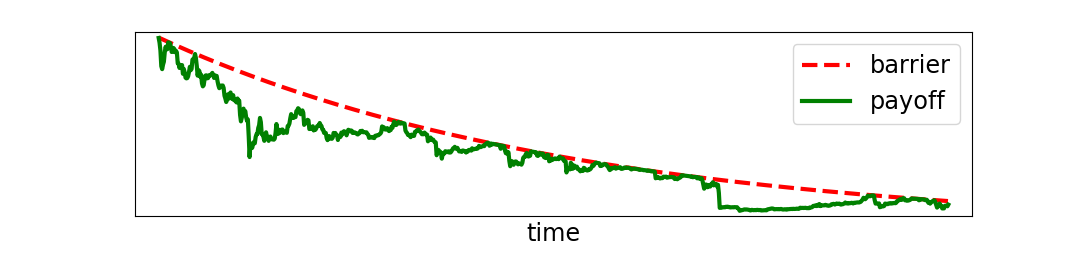
\includegraphics[scale=0.6]{images/exemple_payoff.png} %
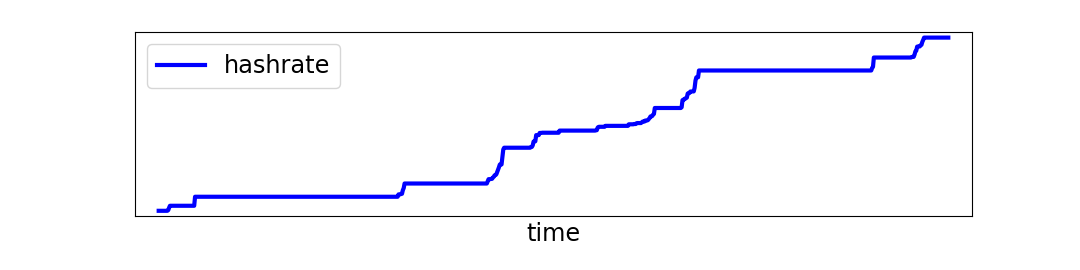
\includegraphics[scale=0.6]{images/exemple_hashrate.png}
\end{figure}

Conditions (i) and (ii) ensure that entry keeps $P_t$ below the entry barrier $\overline{P}_t$; while condition (iii) ensures that no individual miner will find it profitable to deviate from the entry policy.
Conjecturing the properties of the equilibrium greatly simplifies the analysis
since we only have to verify that they are indeed satisfied by the entry strategies. From a formal standpoint, the fundamental difference between our equilibrium
and the one studied by \citeauthor{CaballeroPyndick} (\citeyear{CaballeroPyndick}) is that, due to embodied technological progress,
the investment and the operating costs decrease over time. Hence the entry barrier $%
\overline{P}_{t}$ cannot remain constant. However, if we impose Assumption %
\ref{hyp:rate_TP}, so that mining efficiency improves at a constant rate, we
can solve for the equilibrium in the space of detrended payoffs and
recover a flat barrier.


\begin{prop}
\label{prop:industry-eq} Assume that assumptions \ref{hyp:continuous_update}, \ref{hyp:GBM}%
, \ref{hyp:keep-going} and \ref{hyp:rate_TP} hold. Then there
exists an industry equilibrium $\left(P_t,\overline{P}_t\right)$ such that $P_t$
is a GBM reflected at $\overline{P}_t=\overline{P}_0/A_t$ where\footnote{%
Note that, when $\alpha =r$, $\overline{P}_{0}=\left(I_{0}+\frac{C_0}{r}%
\right)\left( \alpha +a+\frac{\sigma ^{2}}{2}\right)$.}
\begin{equation}
\overline{P}_{0}=\frac{ (r-\alpha )\beta}{\beta -1}\left[I_{0}+\frac{C_0}{r}%
\right], \text{ and } \beta= \text{{\scriptsize $\frac{\frac{\sigma^2}{2}%
-\alpha -a+\sqrt{\left(\alpha +a-\frac{\sigma^2}{2}\right)^2+2\sigma^2%
\left(a+r\right)}}{\sigma^2}$}}>0.  \label{eq:def_barrier}
\end{equation}
\end{prop}

A typical equilibrium is illustrated in Figure \ref{Fig_Eq}. The upper-panel
reports an arbitrary sample path for the payoff process $(P_t)_{t\geq 0}$.
Payoffs follow the changes in block rewards and thus behave as a GBM
until they hit the reflecting barrier $\overline{P}_t$. Such events trigger
market entry, as shown in the lower-panel. The resulting increase in
hashrate raises the difficulty of the mining problem, and so pushes
payoffs down until market entry is not anymore profitable. The entry barrier
decreases at the rate of technological progress because it corresponds to
the pace at which both investment and operating costs fall over time.

\emph{Comparative statics.---} To get some intuition about the impact that each parameter
has on the entry barrier, it is useful to consider the hypothetical
situation where further entries are precluded. Then the marginal
miner is also the last one to ever enter the market. Provided that $r>\alpha$, the value
of the last entrant is positive
whenever $P_0>\overline{P}^{last}_0 \equiv (r-\alpha )\left[I_{0}+ C_0/r\right]$.\footnote{If
market entry is forbidden, $P_t$ obeys the same law of motion as $R_t$ so that
$$V^{last}_0=\int_{0}^{\infty}e^{-rs}\mathbb{E}_0\left[P_t\right]dt-\left[I_{0}+ \frac{C_0}{r}\right]=\frac{P_0}{r-\alpha}-\left[I_{0}+ \frac{C_0}{r}\right].$$}
Comparing the thresholds with and without entry, we see that $\overline{P}_0=[\beta/(\beta -1)]\overline{P}^{last}_0>\overline{P}^{last}_0$.
The break-even payoff is higher under free entry because the arrival of new miners ensures that future payoffs are reflected downwards
when they reach the entry barrier $\overline{P}_0$. The term $\beta/(\beta -1)$ measures the negative impact that entries have on the value of the marginal incumbent.

Differentiating the expression of $\overline{P}_0$ in (\ref{eq:def_barrier}),
we find that $\partial \overline{P}_0/\partial a>0$ and $\partial \overline{P%
}_0/ \partial r>0$. If technological progress accelerates, miners' revenues
shrink more rapidly because there will be even more entries in the future. Hence
entrants have to earn more early on, which raises the entry
barrier. A similar mechanism explains the impact of $r$ since
future revenues are discounted at a higher rate when $r$ goes up.
Not surprisingly, an increase in the average growth rate $\alpha$ of the
block rewards incentivizes entry as $\partial \overline{P}_0/\partial \alpha<0
$. Finally, the volatility of payoffs $\sigma$ discourages entry since $%
\partial \overline{P}_0/\partial \sigma>0$. Note that this is not due
to an increase in the value of waiting because the perfectly competitive
structure of the industry rules out such an option: Competitors would
preempt any procrastination beyond the zero expected profit threshold.
Instead, the negative impact of $\sigma$ on entry is mechanical.
Given that payoffs are truncated from above by the reflecting barrier, an
increase in their spread automatically lowers their expected value.
Quantitatively, the rate of technological progress $a$ has, by far, the
largest effect on $\overline{P}_0$.

\subsection{Extensions}
\label{subsec:Halvings}

We now generalize our model so as to take into account the delivery lags for mining hardware,
and the halving of block rewards every four years.

\emph{Time-to-build.---} We have assumed that miners can enter the market immediately.
In practice, however, new hardware have to be delivered and
installed. Each step increases the lapse of time separating entry from actual production.
When it requires $\delta$ years to effectively become operational, prospective entrants at date $t$ have to forecast
their revenues starting from $t+\delta$. Hence they have to
take into account the price fluctuations that may ensue during the delivery period,
as well as the amount and arrival times of hardware in the delivery pipeline.

To reduce the dimensionality of the state space, we follow the approach proposed by \citeauthor{Grenadier2000} (\citeyear{Grenadier2000}).
Let $H_t$ denote the amount of "committed hashrate", that is all the mining units which are either
already operational, or on their way to being delivered. Given that all orders
will be installed $\delta$ years from now, the hashrate of the network when today's
orders become operational will be equal to the current amount of committed hashrate, i.e. $Q_{t+\delta}=H_t$.
Hence the relevant state variable from the standpoint of entrants is not anymore $P_t=R_t/Q_t$,
but instead $P^{\delta}_t \equiv R_t/H_t$. We show in the Technical Appendix \ref{app:T2B} that equilibrium
strategies are functions of $P^{\delta}_t$ only, and that the mining market
is in equilibrium when $P^{\delta}_t$ is a reflected GBM.

\begin{prop}
\label{prop:industry-eq-T2B} Assume that assumptions \ref{hyp:continuous_update}%
, \ref{hyp:GBM}, \ref{hyp:keep-going} and \ref{hyp:rate_TP} hold. Furthermore, assume
that market entry is delayed by the time-to-build $\delta$. Then there
exists an industry equilibrium $\left(P^{\delta}_t,\overline{P}^{\delta}_t\right)$ such that $P^{\delta}_t = R_t/H_t$
is a GBM reflected at $\overline{P}^{\delta}_t=\overline{P}^{\delta}_0/A_t$. The entry barrier
is related to that of the model without time-to-build by the following equation
\begin{equation}
\overline{P}^{\delta}_t=e^{\left(r-\alpha\right)\delta}\overline{P}_t\left[K_t/K_t^{\delta}\right],  \label{eq:def_barrier_T2B}
\end{equation}
where $K_t\equiv I_{t}+C_t/r$ denotes the overall costs of entry in the model without delay, and $K_t^{\delta} \equiv K_t-(1-e^{-r\delta})C_t/r$.
\end{prop}
\begin{proof}
  See the Technical Appendix \ref{app:T2B}.
\end{proof}

The expression of the entry barrier with time-to-build differs from that
of the baseline model in two respects. First, overall costs of entry $K_t^{\delta}$ are slightly lower because
they are evaluated at the time of the entry decision. Since entrants have to wait $\delta$ years
to start mining, their operating costs $C_t/r$ are multiplied by the discount factor $e^{-r\delta}$.
Second, the barrier without delay is rescaled by $e^{\left( r-\alpha \right)\delta}$
because it is optimal to enter when the expected value of payoffs in $\delta$ years is equal to the discounted
threshold, $e^{r\delta}\overline{P}_t$. Since
$\mathbb{E}_t\left[P_{t+\delta}\right]= e^{\alpha \delta}P^{\delta}_{t}$, setting $\mathbb{E}_t\left[P_{t+\delta}\right]= e^{r\delta}\overline{P}_t$ indeed implies that $P^{\delta}_{t}=e^{\left(r-\alpha\right)\delta}\overline{P}_t$.\footnote{The relationship between the expectation
of $P_{t+\delta}$ and $P^{\delta}_{t}$ holds true because $Q_{t+\delta}=H_{t}$, so that
$$\mathbb{E}_t\left[P_{t+\delta}\right]=\mathbb{E}_t\left[\frac{R_{t+\delta}}{Q_{t+\delta}}\right]
=\frac{\mathbb{E}_t\left[R_{t+\delta}\right]}{H_{t}}= e^{\alpha \delta}P^{\delta}_{t}.$$}

Note, however, that the models with and without delays are not as similar as their descriptions might suggest.
The solution of the baseline model is Markovian since knowing the
current hashrate and Bitcoin price is enough to forecast the evolution
of the network hashrate. By contrast, the solution of the model with time-to-build is path dependent
since forecasts over the next $\delta$ years are conditional on all the
purchase orders that were placed over the previous $\delta$ years.

%
%\begin{equation}
%\overline{P}^{\delta}_{0}=\frac{\beta (r-\alpha )}{\beta -1}\left[I_{0}+\frac{C_0}{r}%
%\right], \text{ and } \beta= \text{{\scriptsize $\frac{\frac{\sigma^2}{2}%
%-\alpha -a+\sqrt{\left(\alpha +a-\frac{\sigma^2}{2}\right)^2+2\sigma^2%
%\left(a+r\right)}}{\sigma^2}$}}>0.  \label{eq:def_barrier_T2B}
%\end{equation}

\emph{Halvings.---} Another limitation of our baseline model is that
it ignores the inclusion in Bitcoin protocol
of a feature which divides by two the number of coins issued per block.
These so-called \emph{halvings} are triggered every 210,000 blocks to ensure that the supply of
bitcoins converges to a finite limit, namely 21 millions. Halvings generate
discontinuities in the paths of $R_{t}$ that are inconsistent with the GBM
specification. To take them into account, one has to replace Assumption $\ref{hyp:GBM}$ with Assumption $\ref{hyp:halvings}$
according to which block rewards are halved every four years.

\begin{hyp}
\label{hyp:halvings} The block rewards are given by $R_{t}=h_{t}\tilde{R}_{t}$%
. $\tilde{R}_{t}$ follows a GBM while $h_{t}=\left(\frac{1}{2}%
\right)^{\left\lfloor t/4\right\rfloor}$, where $t$ measures the number of
years elapsed since the inception of Bitcoin, and $\lfloor x
\rfloor = \mathop{\max}\limits_{n \in \mathds{N}} \{n \leq x\}$.
\end{hyp}

Assumption \ref{hyp:halvings} slightly simplifies the halving process.
First, the reward a miner gets when she finds a block is not exactly divided
by two after each halving because it includes transaction fees on top of new
coins. But the discrepancy is not very important in practice, as transaction fees
account for a residual share of block rewards.
Second, halvings do not occur every four years, but
instead every 210,000 blocks. Counting years is a way to approximate elapsed
time because Bitcoin protocol adjusts the difficulty of the hashing
problem every two weeks on average. It is shown in the Technical Appendix \ref{app:test_cont_update} that, indeed, the updating
rule manages to keep the block generation rate close to one every 10 minutes.

Halvings render the optimization problem of miners non-stationary: the closer they are to
the halving date, the lower their expected payoffs. This
implies that we have to rely on
numerical methods because the entry barrier does not anymore admit a closed-form solution.
Starting from the
analytical solution derived in the proof of Proposition \ref{prop:industry-eq}, we proceed by backward induction
and use a
finite-difference procedure to approximate the entry rule. As the horizon increases,
our algorithm quickly converges towards an entry barrier that is
independent of the number of future halvings.\footnote{%
More precisely, the entry barrier turns out to be stable after four
iterations. We use finite-difference methods to approximate the
Hamilton-Jacobi-Bellman equations satisfied by the value functions of
miners. We rely on the implicit Euler scheme in order to ensure that the
approximation is stable. The system of linearized equations is solved using
a generalization of the Gauss-Seidel iterative method known as the
successive-over-relaxation method.}


\section{Calibration}

\label{sec:calibration}

\subsection{Data}
\label{ssec:Data}

\begin{figure}[t]
\caption{Miners Revenues $R$ and Network Hashrate $Q$}
\label{fig:R-Q}
\centering
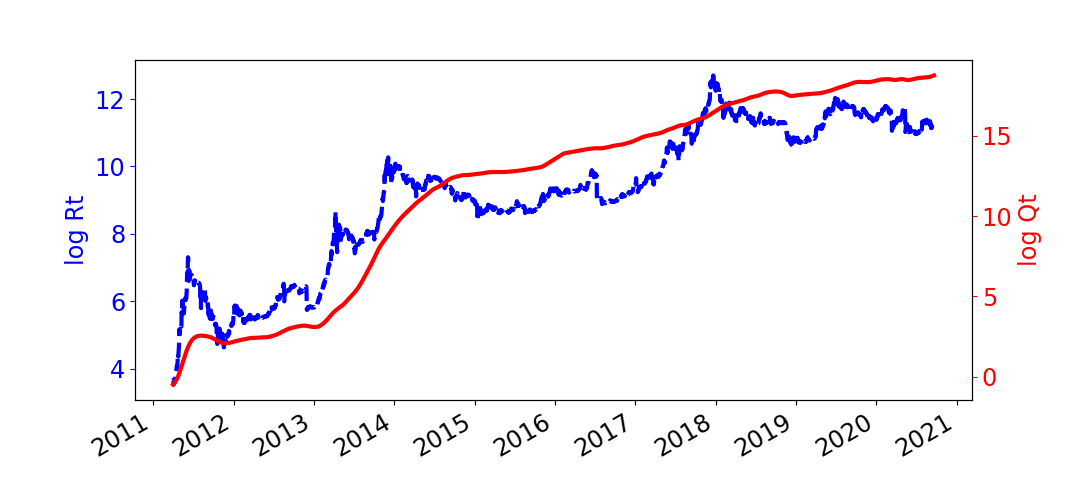
\includegraphics[scale=0.575]{images/R_Q.png}
\caption*{\footnotesize{\textsc{Note: $R_t$ is computed using information collected on coindesk.com and btc.com. $Q_t$
is measured in Terahash per second. Its value is inferred using the procedure described in Appendix \ref{app:estimation_Q}.}}}
\end{figure}

We now show that feeding our model with exchange rate data
allows one to accurately predict the evolution of the network hashrate. For
this purpose, we need to infer the miners' payoffs $P_t=R_t/Q_t$. Remember
that the numerator, $R_t$, is equal to the value of new coins plus the
transaction fees. The number of created coins per block is specified by the
protocol while Bitcoin exchange rate against the dollar is directly available from \href{https://www.coindesk.com}%
{coindesk.com}.\footnote{%
There are many different exchanges and the exchange rate varies a bit across
them. In the Technical Appendix \ref{Bitcoin price data}, we check the validity of coindesk data by comparing them
to a weighted average measure over 17 exchanges. Since the two series are virtually indistinguishable,
we select the one that is most easily accessible.} The transaction fees are recorded in Bitcoin's
blockchain and can easily be retrieved from \href{https://www.btc.com}{%
btc.com}. Thus all the components of $R_t$ are readily
available. By contrast, the network hashrate $%
Q_t$ is not directly observable. It must be estimated using the theoretical
probability of success and the number of blocks found each day. Given that
we are not primarily interested in statistical inference, we relegate the
description of our estimation procedure to the Technical Appendix \ref{app:estimation_Q}
and save on notation by using $Q_t$ to denote our estimate, although its
time series only approximates the true hashrate. We show in the Technical Appendix
\ref{app:estimation_Q} that the approximation is accurate. We update the value
of $Q_t$ on a daily basis and, since there are on average $144$ blocks mined
every day, the expected payoffs per day are given by $P_t=144 \times R_t/Q_t$.

We report the series followed by $R_t$ and $Q_t$ in
Figure \ref{fig:R-Q}. There is a clear correlation between the two
variables. Our model suggests that their structural relation should become
apparent if one takes the ratio of the two series and detrend it at the rate
of technological progress $a$. Then the resulting series should behave as a
reflected GBM. For many years, improvements in the processing industry have followed Moore's law, according to which processor speed doubles every two years. We expect improvements in the mining technology to outpace those in
processing speed because miners came up with a series of innovations which
allowed them to leverage their computing power. Thus, at this stage we pick a rate of techological progress slightly  faster than Moore's law (1.5 times faster). We will refine our
guess later on by calibrating the value of $a$. 

\begin{figure}[]
\caption{Detrended Payoff Series}
\label{fig:P_tilde_Moore}\centering
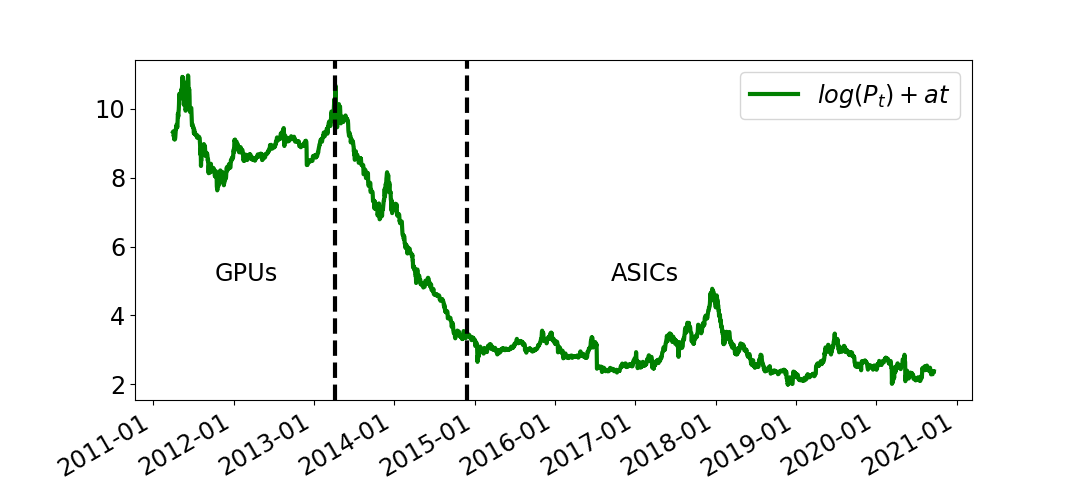
\includegraphics[scale=0.65]{images/P_tilde.png}
\caption*{\footnotesize{\textsc{Note: $P_t$ is equal to the daily network revenues $144*R_t$ divided by $Q_t$.}}}
\end{figure}

%\begin{figure}[]
%\label{fig:P_tilde_Moore_new}\centering
%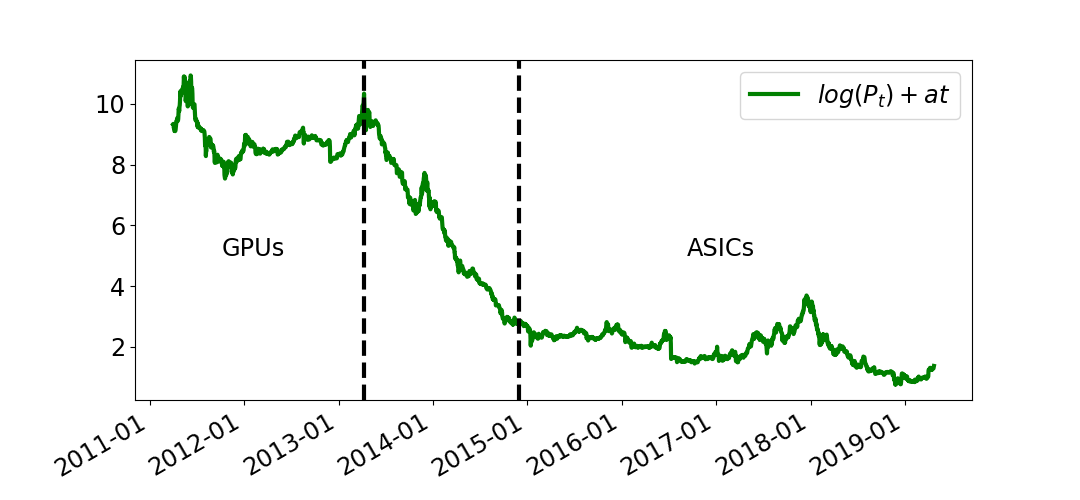
\includegraphics[scale=0.55]{images/P_tilde_Moore_new.png}
%\caption*{Note: $P_t$ has been computed dividing $144R_t$ (the daily network revenue) by $Q_t$.}
%\end{figure}

The payoff series detrended at the rate implied by Moore's law is reported in Figure \ref%
{fig:P_tilde_Moore}. It exhibits two stationary regimes, with a break in the
middle where payoffs decreased regularly until they reached a lower plateau.
At first, this pattern does not seem to square with our model. But if we
focus on the date at which the break initiates, we realize that it coincides
with a fundamental change in the mining technology.

Early on, miners used to mine with their own computers. Around mid-2010, they
realized that Graphical Processing Units (GPU) were much more efficient. One
year later, miners started to use Field Programmable Gate Arrays (FGPA) and,
since 2013, they mostly mine with Application Specific Integrated Circuits
(ASIC). ASICs are also called mining rigs because their sole purpose
is to solve Bitcoin's hash-puzzle.

The first ASIC was delivered to Mr. Jeff Garzik on January 30th 2013.\footnote{See \url{https://bitcoin.stackexchange.com/questions/40944/when-did-the-asic-mining-era-begin}}
Since this revolution in the mining technology boosted the rate of technological progress well
above its long-run trend, its propagation among miners violates Assumption \ref{hyp:rate_TP}, and
so, one should not expect the predictions of our model to be verified
during the transitory phase. We
therefore leave aside the lapse of time where
miners switched from GPUs and FPGAs to ASICs, and focus instead on the two
subperiods where miners used the same technology. More precisely, during the
first period, which ranges from 2011/04/01 to 2013/01/31,\footnote{We excludes the very early
history of Bitcoin because it features an unstable block generation rate (see the Technical Appendix \ref{app:test_cont_update}).}
miners mainly mined with GPUs;
while they mostly relied on ASICs from 2014/10/01 onwards.
Our second subperiod ranges from 2014/10/01 to 2017/03/31.
It does not include our most recent data because they cover an episode of trading frenzy during which Bitcoin experienced
a giant bubble followed by a sudden burst.
We will analyze this event and its aftermath in Section \ref{sec:Bubble}.

Buying an ASIC is an irreversible decision because it can be
used for cryptocurrency mining only. Hence, if the price of Bitcoin falls, ASICs
cannot be resold for profit because all miners face the same returns.
The irreversibility assumption is less obvious for GPUs. Yet, the calibrated values of $a$ reported below
in Table \ref{table:calibration_halving} show that GPUs were facing a very high rate of obsolescence.
This suggests that irreversibility is also a sensible approximation for GPUs, as
nobody would buy them second hand without a tremendous discount. The conjecture
is confirmed by the analysis in the Technical Appendix \ref{app:totally reversible investments}, where we calibrate a model with reversible investment
and find that it fails to match the data.

\subsection{Calibration strategy}
We calibrate the parameters for each
subperiod. The baseline models is parsimonious enough to rely on six parameters only:
the deterministic trend $\alpha$ of rewards and their volatility $\sigma^2$,
the rate of technological progress $a$, the discount rate $r$, the price $%
I_0 $ of one unit of hashpower bought at time 0, and the operating cost $%
C_0 $ of that same unit. The first two parameters can be directly estimated
using $R_t$ only. Under Assumption \ref{hyp:GBM}, the log
returns are independent and follow a normal distribution with mean $\mu
\equiv \alpha-\sigma^2/2$, and variance $\sigma^2$, which we estimate by
maximum likelihood (see Technical Appendix \ref{app:test_GBM}).

%Assumption \ref{hyp:GBM} is satisfied except for the fact that the tails are too fat and the volatility parameter does not remain constant over time. (See Appendix \ref{app:test_GBM}). The change in the volatility parameter is handled by the split of our sample in two subperiods. As for the too fat tails, this is a well-known and usual problem
%shared by many financial series. Yet, like much of the financial literature,
%we would really like to avoid working with a more realistically modeled
%exchange rate since the equations become much more complicated and certainly
%not tractable. The strength of our model is that it is simple enough to
%yield a closed form, which enables us to estimate many parameters of
%interest. In this article, the exchange rate is not in itself an object of
%particular interest. We only need to show the existence of a reflecting
%barrier for the payoff process. The GBM assumption is the most natural and
%common way to obtain this result. Even though the model does not stick to
%the reality on that point it still manages to reproduce the data very well
%despite its parsimony, as the rest of this section shows it. The relative
%failure of assumption \ref{hyp:GBM} will only affect the fit of the model in
%the short run. As discussed below, after one of those extreme returns,
%miners cannot immediately increase the hashrate as much as the model would
%predict and payoffs temporarily exceed the barrier.

The rate of technological progress, $a$, and the reflecting barrier, $%
\overline{P}_0$, are set to minimize a (pseudo)distance between the observed
and the simulated paths of the hashrate. A direct consequence of our
equilibrium definition is that $Q_t=\max\left(Q_{t-1},\frac{R_tA_t}{%
\overline{P}_0}\right)$ for all $t$. This condition provides us with a
straightforward way to simulate the hashrate for any sample with $T$
observations:

\begin{enumerate}
\item Set the initial value of the simulated hashrate $Q^{sim}_{0}$ equal to
its empirical counterpart, i.e. $Q^{sim}_{0}:=Q_0$.

\item Update the simulated hashrate as follows $Q^{sim}_t:=\max%
\left(Q^{sim}_{t-1},\frac{R_tA_t}{\overline{P}_0} \right)$, for $t=1,\dots,T$%
.
\end{enumerate}
Since $(R_t)_{t \geq 0}$ and $Q_0$ are observed, the minimization procedure boils
down to finding the value of $a$ and $\overline{P}_0$ such that
\begin{equation}  \label{eq:estimation_a_B}
(\hat{a},\hat{\overline{P}}_0) \in \mathop{argmin}\limits_{(a,\overline{P}%
_0) \in \mathbb{R}\times \mathbb{R}_+} \sum_{t=1}^T\left(\frac{%
Q_t-Q_t^{sim}(a,\overline{P}_0)}{Q_t}\right)^2.
\end{equation}

Unfortunately, the other three parameters $\{r,I_0,C_0\}$ cannot be separately identified.
We will describe in Section \ref{sec:Extensions} a model where investment is
reversible, and explain how it enables us to separate the investment cost, $I$,
from the operating cost, $C$. At this stage, the best we can do
is to fix $r$, and recover the overall costs of entry at the beginning of each subperiod, $K_0\equiv
I_0+C_0/r$, by equating the expression for $\overline{P}_0$ in (\ref%
{eq:def_barrier}) with the calibrated $\hat{\overline{P}}_0$. The arbitrary
choice for the discount rate, $r$, turns out to be relatively unimportant
because the term $(r-\alpha)\beta/(\beta -1)$ in (\ref{eq:def_barrier}), and
thus the entry costs, are rather inelastic with respect to $r$.\footnote{%
In the second period, setting $r=0.2$ yields $K_0=$ \$1639, while $r=0.05$
yields $K_0=$ \$1934.}

\subsection{Results}
\label{Ssec:Results}

\emph{Calibrated parameters.---} The parameters resulting from our calibration
strategy are reported in Table \ref{table:calibration_halving}, their values
expressed as yearly rates whenever applicable.\footnote{%
For example, the calibrated values of $a$ means that the price of a new hardware has
been on average divided by $\exp(a)$ every year during each subperiod.}
The standard errors are obtained using block bootstrap,
an estimation technique that is more suited to time series
than standard bootstrap.\footnote{The block bootstrap procedure is described in the Technical Appendix \ref{app:block_bootstrap}.}

We first present the trend and volatility of the reward process. Both
coefficients are independent of the modelling strategy
since they are directly estimated by maximum likelihood on the rewards series $R_t$.
The average growth rate of rewards, $\mu$, decreased a lot between the
two periods of study. As one would expect, early buyers of bitcoins earned
higher returns. Information about their profits pushed the demand for
bitcoins which raised the exchange rate even more. But the extremely high
returns observed at the beginning became harder to sustain as the market
capitalization grew from a negligible amount, to nearly \$ 20 billions by the
end of our sample. In spite of this cooling process, investing in Bitcoin
remained extremely profitable. These tremendous
returns have led many observers to announce the imminent collapse of Bitcoin.%
\footnote{%
According to the website \href{https://99bitcoins.com/bitcoinobituaries/}{%
bitcoinobituaries}, by August 2019,
371 opinion pieces had predicted the death of
Bitcoin.} Whether or not such predictions will eventually be vindicated is
beyond the scope of this paper, but our estimates for the volatility
coefficient $\sigma$ indicate that there was no obvious arbitrage
opportunity; investors willing to bet on Bitcoin also had to bear a huge
risk. Even though the volatility of rewards was divided by three in the
second period, its value remained an order of magnitude higher than its
counterpart for the S\&P 500.\footnote{%
We find that, for the S\&P 500, $\sigma^2=0.053$ for the first period and $%
\sigma^2=0.027$ for the second period}



\begin{table}[h]
\caption{Calibrated Parameters}
\label{table:calibration_halving}
\begin{center}
\scalebox{.775}{
\begin{tabular}{lcl|ccc|ccc}
\hline \hline
\multicolumn{2}{l}{Parameters} & Interpretation & & 1st period & & & 2nd period & \\
\hline \hline
\vspace{-1.5ex}& & & & & & & & \\
\multicolumn{3}{l|}{\textsc{A. Maximum Likelihood}} & & & & &  &\\
\multicolumn{2}{l}{$\alpha$} & Trend $R_t$     & & 2.38 & & & 0.46 &  \\
\multicolumn{2}{l}{$\sigma^2$} & Volatility $R_t$  & & 1.95 &   & & 0.54 &  \\
\vspace{-1.5ex}& & & & & & & & \\
\hline
\vspace{-1.5ex}& & & & & & & & \\
\multicolumn{3}{l|}{\textsc{B. Calibration}}& Baseline & Halvings & Time-to-Build & Baseline & Halvings & Time-to-Build \\
\multicolumn{2}{l}{ a} & Rate of TP & 1.18   & 1.29   & 1.10   & 0.76   & 0.85   & 0.90  \\
&    &            & (0.50) & (0.43) & (0.42) &(0.12)  & (0.13) & (0.13)\\
\multicolumn{2}{l}{$K_0$} & Total Costs & \$ $5.6$ mn   &  \$ $5.3$ mn & \$ $4.7$ mn    & \$$1,825 $   & \$$1,655$& \$$1,465$\\
&        &             & (\$ $16$ mn)  & (\$ $8.9$ mn)& (\$ $17.8$ mn) & (\$199)      & (\$83)   & (\$232)  \\
\multicolumn{2}{l}{$\delta$} & Time-to-Build    &               &            &  11.5 days   &            &          & 46.5 days \\
&           &      &               &            &  (9.24 days) &            &          & (27.8 days)\\
\hline\hline
\end{tabular}}
\end{center}

\scalebox{.775}{
\begin{tabular}{lcl|ccc}
\hline \hline
\multicolumn{2}{l}{Parameters} & Interpretation & & 3rd period & \\
\hline \hline
\vspace{-1.5ex}& & & & & \\
\multicolumn{3}{l|}{\textsc{A. Maximum Likelihood}} & & & \\
\multicolumn{2}{l}{$\alpha$} & Trend $R_t$     & & 0.27 & \\
\multicolumn{2}{l}{$\sigma^2$} & Volatility $R_t$  & & 0.80 & \\
\vspace{-1.5ex}& & & & & \\
\hline
\vspace{-1.5ex}& & & & & \\
\multicolumn{3}{l|}{\textsc{B. Calibration}}& Baseline & Halvings & Time-to-Build \\
\multicolumn{2}{l}{ a} & Rate of TP & $0.76$   & $0.95$   & $0.65$ \\
&    &            & ($0.34$) & ($0.31$) & ($0.32$)\\
\multicolumn{2}{l}{$K_0$} & Total Costs & \$ $182$ &  \$ $173$ & \$ $160$ \\
&        &             & (\$ $203$)  & (\$ $122$)& (\$ $152$)\\
\multicolumn{2}{l}{$\delta$} & Time-to-Build  & & &  $43.5$ days \\
&           &      &               &            &  ($21.3$ days) \\
\hline\hline
\end{tabular}
}

\footnotesize{Note: Calibrations based on an annual discount rate $r=10\%$. $K_0$ is the calibrated total cost per Terahash-second at the first day of
each subperiod.
All parameters expressed as yearly rates except the time-to-build, $\delta$, which is expressed in days.
Standard errors from block bootstrap in parenthesis.}

\end{table}


According to Moore's law, the price of one unit of hashpower should be divided by two
every two years. Hence it implies that the rate of technological progress
$a$ should be close to $\log(2)/2\approx0.35$, a number well below the calibrated values of $a$ reported in Table \ref{table:calibration_halving}.
The mining technology
progressed at a faster pace than the one predicted by Moore's law because miners
were able to implement innovations specific to the hash-puzzle on top of
the raw increase in computing power. Our calibrated parameters also indicate
that the rate of technological progress slowed down considerably in the
second period, thus suggesting that improvements specific to the mining problem became harder to
unearth as the technology matured.

Comparing the parameters across models, we see that introducing halvings
lowers the overall costs of entry, $K_{0}$,
but raises the rate of technological progress, $a$. The decrease
in $K_{0}$ is quite intuitive: Since halvings lower expected revenues,
free entry holds when mining costs are smaller. The reason why $a$
increases is more subtle. The adjustment corrects the
misspecification of the baseline model that leads to an overestimation of the
hashrate around the halving dates. This is why the minimization procedure,
when applied to the baseline specification without halvings, generates a
negative bias for $a$ because it uses this parameter to reduce the discrepancies
around the halving date.

The delivery lags of the model with time-to-build are
relatively modest: 11.5 days during the first period, and 46.5 days
during the second period.
As expected, the lags are smaller during the first period since GPUs are more commonly available than ASICs. The total costs are lower
with time-to-build than without, a finding that is in line with Proposition \ref{prop:industry-eq-T2B} and the impact of discounting on future profits.
We also notice that the impact of delays on the calibrated rate of technological progress is negative in the first period, but positive in the second period.
Without further data, it is difficult to tell whether this ambiguity is structural, or simply specific to our samples.

Finally, note that the parameters are identified with much higher precision in the second period. Three factors explain why the first period calibration
is so fuzzy. First, Bitcoin price was extremely volatile. Second, Bitcoin experienced a long slump, a period known as the first crypto winter within
Bitcoin community. This resulted in a nearly flat hashrate for most of the sample, as can be seen in Figure \ref{fig:hashrates_halving}.
From the standpoint of our calibration strategy, this means that there are relatively few data points where free entry binds, making it
difficult to pin down the structural parameters. Finally, the technology was less homogenous during the first period.
In particular, it witnessed the emergence of mining pools. \citeauthor{Cong2018} (\citeyear{Cong2018})
explain why market entry was incentivized by this new opportunity to share risk, thus generating a positive bias in our calibration
of the rate of progress.
For all these reasons, we henceforth treat the second period as our sample of reference.

\emph{Predicted vs actual hashrate.---} The calibration procedure provides us
with an estimate for the reflecting barrier, $\overline{P}_0$, as well as
for its trend, $a$. Using these two values, we can run the two-step
algorithm described above to simulate the network hashrate $%
Q^{sim}$. We report the simulated series against their empirical
counterpart in Figure \ref{fig:hashrates_halving}. In spite of its very parsimonious
structure, the baseline model tracks the actual hashrate remarkably well.



\begin{figure}[]
\caption{Simulated vs Observed Hashrates}
\label{fig:hashrates_halving}\centering
\begin{tabular}{cc}
First Period & Second Period \\
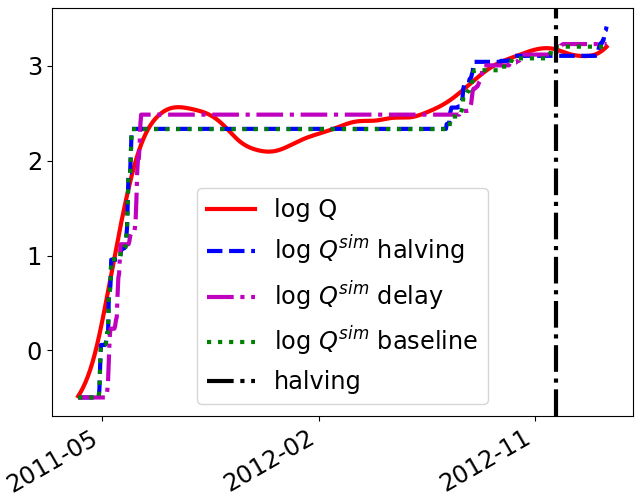
\includegraphics[scale=0.45]{images/Q_all_1.png} & %
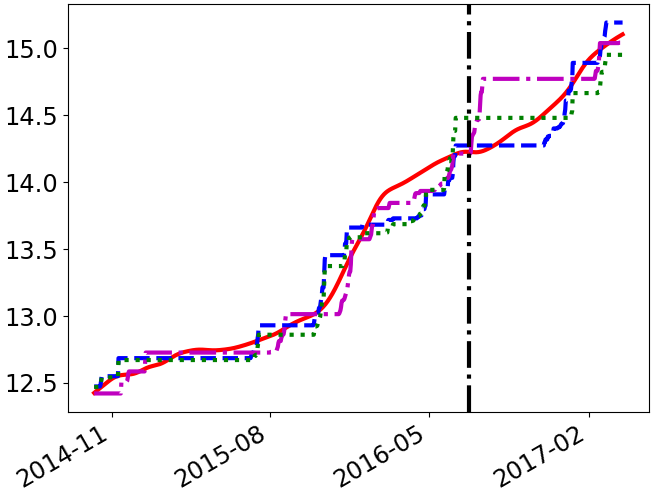
\includegraphics[scale=0.45]{images/Q_all_2.png}%
\end{tabular}%
\end{figure}


We nonetheless notice some temporary discrepancies. The most striking is around the second
halving date (2016/07/09).
This should not be surprising since miners do not
anticipate halvings in the baseline specification while they certainly do in reality.
Figure \ref{fig:hashrates_halving} shows that this shortcoming is solved by the extended model
with halvings.
However, besides this specific period, the paths generated by the three models
remain very close to each other. Due to the extreme volatility of the exchange rate,
halvings affected miners' behavior only a couple of months ahead. It is actually more intriguing that such a disconnect between the simulation
of the baseline model and the data is not apparent around the first halving date (2012/11/28). According to our model,
miners had a very short investment horizon during the first period because the rate of technological progress was extremely high.

Another noticeable difference between the actual and simulated hashrates
is that the former sometimes decreases, especially during the first period,
while the latter never does. Our models cannot generate any decrease in
hashrate because they are based on the premise that investment is totally
irreversible. We will address this shortcoming in Section \ref{sec:Extensions}
where we allow miners to mothball and scrap their
hardware.


These discrepancies do not invalidate our approach because its objective
was to capture medium to long run adjustments in hashrate, and it
largely succeeds in this respect. Yet one may argue that
such a conclusion is too generous because our procedure minimizes the
distance between the simulation and the data, and so would fit the data
fairly well even if the model were misspecified. Remember, however,
that the baseline model uses only two parameters to
fit times series of 608 and 913 data points. For each
simulation, we start from the initial hashrate and then
let the model run without using intermediate realizations to correct its
output. Hence, any fundamental
misspecification would generate a noticeable gap between the
simulation and the data, at least over some time intervals. The fact that
there is no deterioration of the models' accuracy is therefore a
convincing argument in favor of their validity. We now provide additional evidence in favor of this
interpretation by performing out-of-sample experiments, and by comparing the entry
rules generated by the models with the ones prevailing in the data.


We assess the model's ability to match
out-of-sample data by dividing the second period into a fit period and a
test period. We calibrate $a$ and $\overline{P}_0$ on the fit period only
and find that, even when the fit period is short, the calibrated
values remain close to the ones based on the full sample. Hence the predicted
hashrate stays accurate several years after the end of the fit period, as shown in
the Technical Appendix \ref{app:out_of_sample}.


\begin{figure}[]
\caption{Simulated vs. Observed Payoffs}
\label{fig:payoffs}\centering
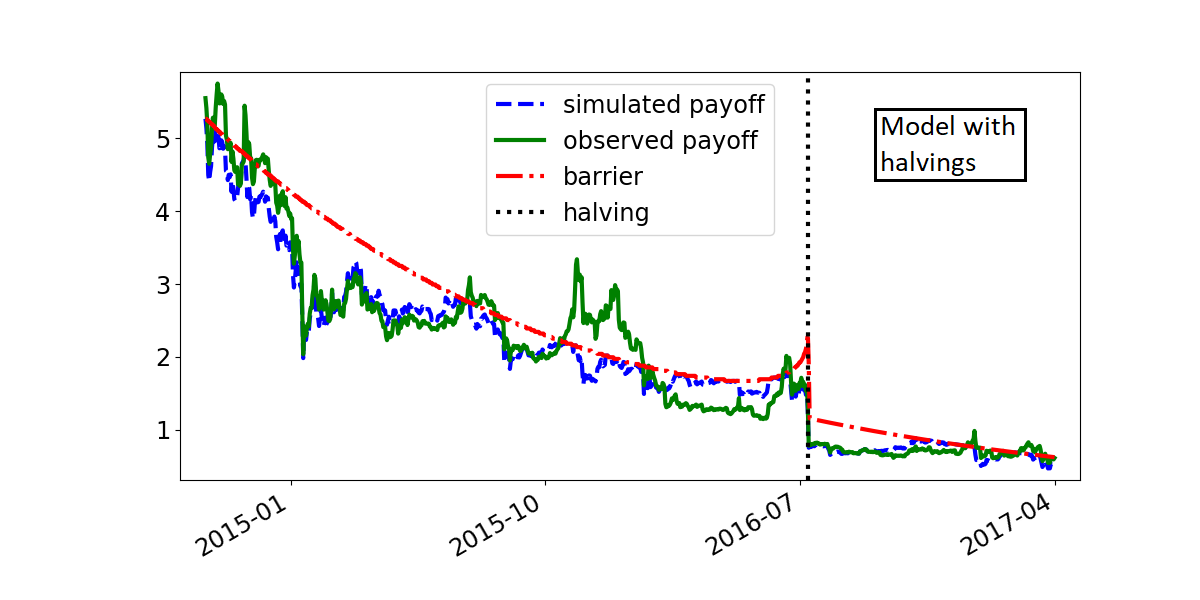
\includegraphics[scale=0.48]{images/P_P_sim_hf_2_wide.png}
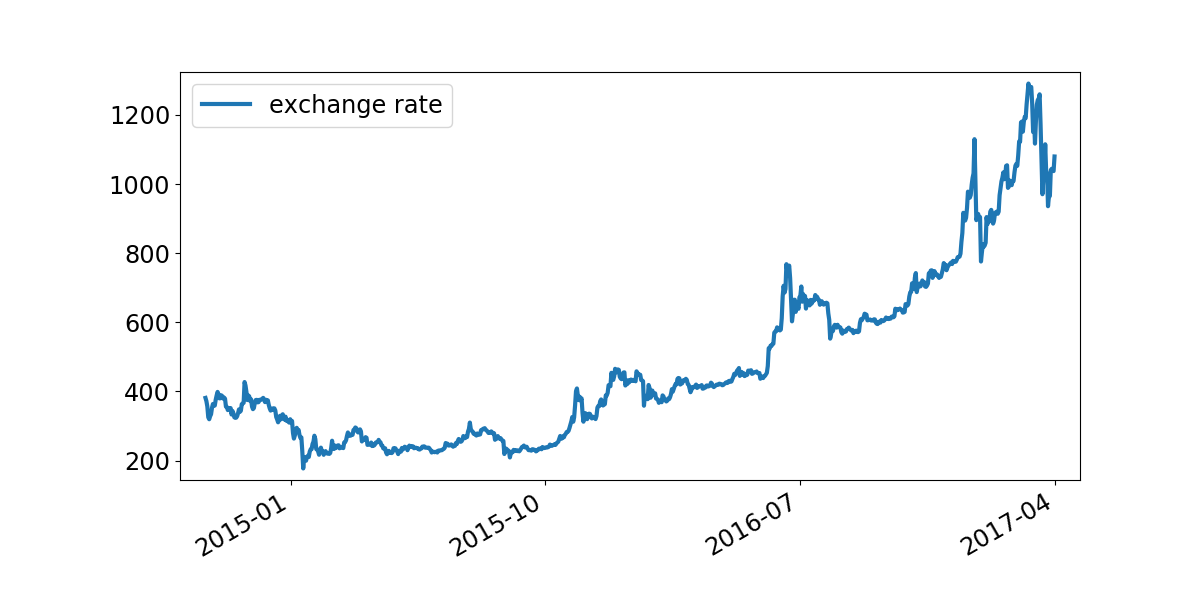
\includegraphics[scale=0.50]{images/cours2_wide.png}
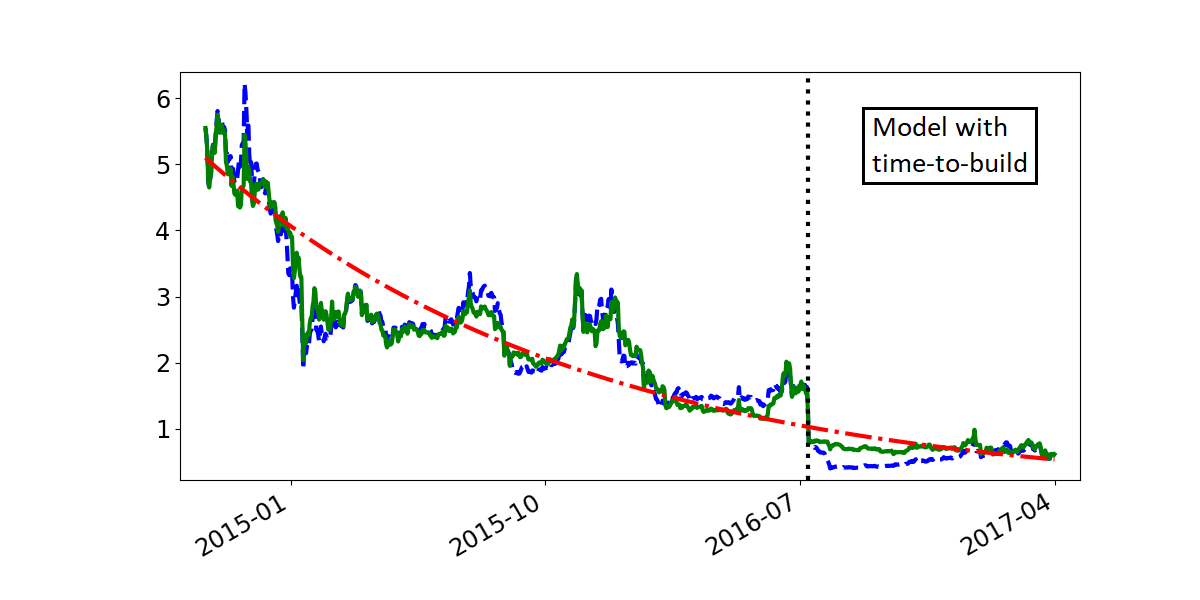
\includegraphics[scale=0.48]{images/P_P_sim_delay_2_wide.png}
\end{figure}



\emph{Inspecting the entry rule.---} Besides assessing the
accuracy of the simulated hashrate, we can also check whether the behavior of payoffs
is consistent with the entry rule. For this purpose, we report in Figure \ref{fig:payoffs}
the simulated and
observed payoffs series, as well as the \bitcoinA / \$ exchange rate to ease interpretation.
For the sake of conciseness, we only report the payoff series of the second period.\footnote{
We show in the Technical Appendix \ref{app:1st_period} that the fit of the payoff series during the first period
is also very convincing.}
The upper-panel of Figure \ref{fig:payoffs} focuses on the model with halvings
whose barrier shifts down by $50\%$ on the halving date. This drop is preceded by a period where the barrier slopes up because
miners anticipate the fall in future revenues, and so, procrastinate further
before entering the market. But
the increase in the barrier becomes noticeable only a
few months before the halving and is therefore not relevant for most of the preceding
period. This might be surprising given that a division by two of revenues
seems like a huge loss; yet one has to put it into perspective by comparing
it to the very rapid obsolescence of hardware, and to the extreme volatility of Bitcoin price.
These two forces imply that a loss of $50\%$ in rewards over a few months was not an
implausible event. Accordingly, as can be seen comparing
the two panels of Figure \ref{fig:hashrates_halving}, the lower the rate of technological progress and the volatility of Bitcoin,
the more noticeable halvings are.

As predicted by our model, observed payoffs remain below the barrier most
of the time and tend to reflect downwards when they reach its vicinity. This
is remarkable since $\overline{P}_t$ was calibrated regardless of
this requirement, fitting the hashrate only. Although the observed and simulated
payoff series are often superimposed,
they differ over some short time intervals.
These discrepancies are usually triggered by extreme increases in
the exchange rate, as can be seen comparing the upper-panel of Figure \ref{fig:payoffs}
with the middle-panel that contains Bitcoin price series. Quite
intuitively, when the exchange rate goes up by 10\% or more in one day,
miners cannot enter the market as
quickly as the model predicts because they are facing, among many other
frictions, delivery and manufacturing delays.

This conjecture is confirmed by the lower-panel of
Figure \ref{fig:payoffs} which reports the payoff series with time-to-build.
The simulation now almost perfectly tracks the data. In particular,
sudden price increases do not anymore drive a wedge between the model and the data.
Instead, they push both series above the entry barrier for a short amount of time.
This is possible in the model with time-to-build because the entry threshold acts
as a reflecting barrier for the committed hashrate, $H_t$, and not for the actual hashrate, $Q_t$.
Hence, a sudden increase in the price of Bitcoin triggers a jump in $H_t$, as new miners
decide to enter the market, but the impact of their decision is delayed by the time-to-build.
This explains why the payoff series tends to revert after a big price surge:
On impact, it follows the price trajectory, and then decreases a few weeks later, once the mining hardware
has been delivered.

To take stock, out-of-sample experiments and inspecting the entry rule
confirm that the baseline model reliably predicts the
evolution of the network hashrate. Yet, its accuracy temporarily deteriorates
around halving dates and after big price surges, two shortcomings that
can be addressed by the introduction of halvings and time-to-build.
These adjustments do not strongly affect the calibrated values of the parameters which
remain rather stable across the three specifications. Having established the
soundness of our approach, we now consider two extensions. The first one will allow us
to separate the investment from the operational costs, while the second
one will enable us to match the 2017 bubble and its aftermath.

\section{Reversible Investment}

\label{sec:Extensions}

\subsection{Mothballing and scrapping options}

The network hashrate never decreases in our simulations because they hinge on the assumption that miners
always keep their hardware in mining mode.
In practice, miners have the
option to switch off their hardware, and they can switch them back on should
mining become profitable again. We now generalize our approach to take these options
into account. We assume that mining hardware can be kept idle
at zero costs. Then the mothballing decision is fully reversible, and as
such does not involve any forward-looking component: Machines are mining
whenever their flow revenues are higher than their operating costs.
Hence the per-period profits at time $t$ of a miner entered at
time $\tau$ are equal to $\max\left(P_t-C_{\tau},0\right)$, and her value
function reads
\begin{equation}  \label{Value_mothball}
V(P_t,\tau)=\mathbb{E}_t\left[\int_t^{+\infty}
e^{-r(s-t)}\max\left(P_s-C_{\tau},0\right)ds\right].
\end{equation}

If there is no technological progress, all miners pay the same operating
costs ($C_{\tau}$ is constant) and thus face the same problem. Then the
industry equilibrium features two reflecting barriers: an upper-barrier
generated by the entry of new miners which pushes payoffs downwards until free
entry is satisfied again, and a lower barrier generated by the exit of
incumbents which pushes payoffs upwards until miners are indifferent between
operating and stopping their hardware.\footnote{%
See \citeauthor{Alvarez} (\citeyear{Alvarez}) for a model with two
reflecting barriers generated by workers entry and exit.} With technological
progress, however, the structure of the industry is much more intricate. Then miners
cannot all be indifferent since they bear different operating costs. The
least productive miners are the first to mothball their hardware, and they
do so until the marginal miner makes zero flow profits. This endogenous
cutoff depends on the distribution of vintages among incumbents. Thus the
law of motion of $P_t$ is not anymore a function of current revenues only, but
also of the vintage distribution. This in turn greatly complicates the
decision of prospective entrants who now have to solve a problem which
includes a distribution function among its state variables.

Instead of following this direct approach, we take the view that
prospective entrants do not have access to the data required to solve the
full information problem. Finding the vintage of all hardware is an
extremely tedious, if not impossible, task. It is therefore quite unlikely
that miners actually looked for this information before investing and, even
if they did, they would only have observed a very noisy measure of the
actual distribution. We assume instead that potential entrants make their
decisions considering only the current value of their flow payoffs. We
establish below the plausibility of this restriction by showing that
mothballing and scrapping have very little impact on the hashrate, so
that entrants cannot significantly benefit from solving the full information
problem. From a formal standpoint, we assume that miners' expectations
satisfy the following Markov property.

\begin{hyp}
\label{hyp:miners_myopic} Let $\mathcal{F}_t\equiv\sigma(P_s;0\leq s \leq t)$
denote the filtration generated by $P$. We assume that, for all measurable
set $A \in \mathbb{R}_+$ and all $s>t$, $\mathbb{P}^e\left(P_s \in A|\mathcal{F}%
_t\right)=\mathbb{P}^e\left(P_s \in A|P_t\right)$, where $\mathbb{P}^e(\omega)$ is the
probability of event $\omega$ as evaluated by potential entrants, and $\mathcal{F}_t$
is the filtration generated by $P_t$.
\end{hyp}

\begin{figure}[]
\caption{Mothballing and Scrapping Regions}
\label{fig:variable_costs}\centering
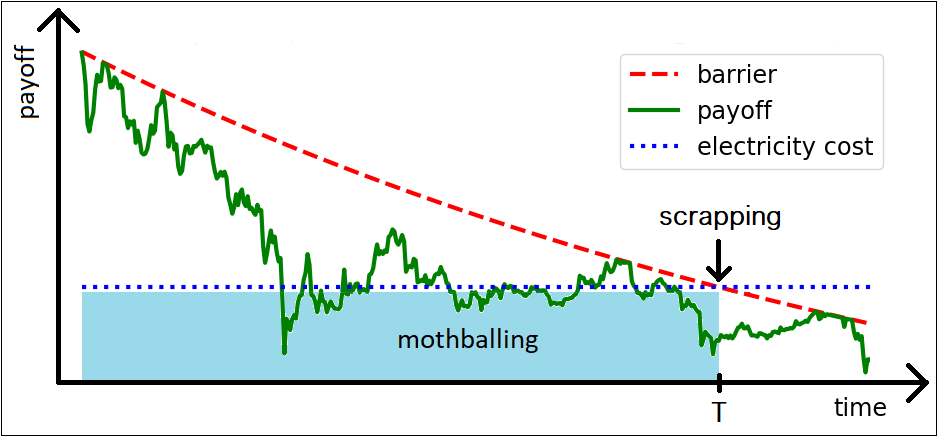
\includegraphics[scale=0.6]{images/cout_variable2.png}
\end{figure}

We show in the proof of Proposition \ref{prop:industry-eq-variable-costs}
that, replacing Assumption \ref{hyp:keep-going} with Assumption \ref{hyp:miners_myopic},
does not fundamentally alter the structure of the equilibrium. It remains
characterized by an entry barrier $\overline{P}_t$ which decays at the rate
of technological progress. Since payoffs are reflected downwards when they
hit the barrier, it will never be profitable to operate a piece of hardware
which is so obsolete that its operating costs exceed the entry barrier. A
typical mining cycle is illustrated in Figure \ref{fig:variable_costs}: Hardware
are mothballed whenever payoffs fall below its operating costs, as
indicated by the colored area; and they are scrapped when the entry barrier
crosses the operating costs.

\begin{prop}
\label{prop:industry-eq-variable-costs} Assume that assumptions \ref%
{hyp:continuous_update}, \ref{hyp:GBM}, \ref{hyp:rate_TP} and \ref%
{hyp:miners_myopic} hold true. Then there exists a $\overline{P}_0 >0$ such
that $\left(P_t,\overline{P}_t=\overline{P}_0/A_t\right)$ is an industry
equilibrium that satisfies the requirements of Definition \ref%
{def:industry-eq}.
\end{prop}

%Although there is no closed form solution for $\overline{P}_0$,
%we can simulate the hashrate by relying on a generalization of the procedure used
%for the baseline model. A significant advantage of the extended model is that
%it disentangles the price of the machines from their operating costs.

\emph{Simulating the hashrate.---} The addition of an exit threshold makes it
impossible to analytically solve for the entry barrier $\overline{P}_t$. Moreover, simulating the hashrate is more
complicated than for the baseline model because one must keep track of the
operating costs, as well as of the activity status of all miners. The
inputs of the algorithm are the block rewards $R_t$, the rate of technological progress $a$, the initial
hashrate, the operating costs and the entry barrier $\left(Q_0,C_0,\overline{P}%
_0\right)$.\footnote{We also need to initialize the vintage distribution of all
active miners. In line
with Assumption \ref{hyp:miners_myopic}, we find that knowing the true distribution
of miners' vintages does not significantly improve forecast accuracy. A series of robustness checks demonstrates that the initial
choice of vintages hardly affects the simulated paths after a couple of days.
We therefore pick a distribution for which the mass of miners of
any vintage is inversely proportional to the price of their hardware, as
would have happened if the environment were deterministic.}

The simulation procedure works as follows. For each day, we start by
deleting from the database all miners whose operating costs are bigger
than the entry barrier since they will never find it profitable to mine in the future.
Then, given the new value of $R_t$, we compute the temporary payoff
faced by miners if the hashrate remains constant. Depending on its value, two
configurations may arise. First, if this temporary payoff is smaller than
the operating costs of the least efficient--i.e. oldest--active miner, we
know that some miners should switch off their hardware. Thus we let the
least efficient miners mothball their hardware, and update the temporary
payoff until no active miner prefers to remain idle. Alternatively, if the
temporary payoff is higher than the operating costs of the most efficient
inactive miner, we know that some miners should switch on their hardware.
Finally, if all incumbents are active and the temporary payoff is still
bigger than the entry barrier, we let new miners enter the market until the
temporary payoff is equal to the entry barrier.

\begin{figure}[]
\caption{Simulated vs Observed Hashrates}
\label{fig:hashrate_variable_costs}\centering
\begin{tabular}{cc}
First Period & Second Period \\
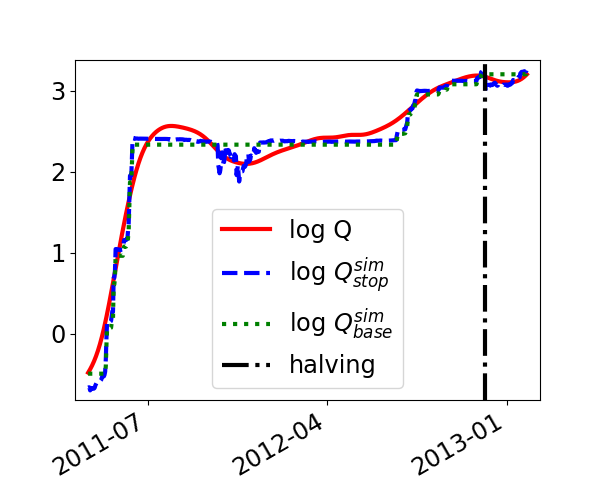
\includegraphics[scale=0.54]{images/Q_Q_sim_stop1.png} & %
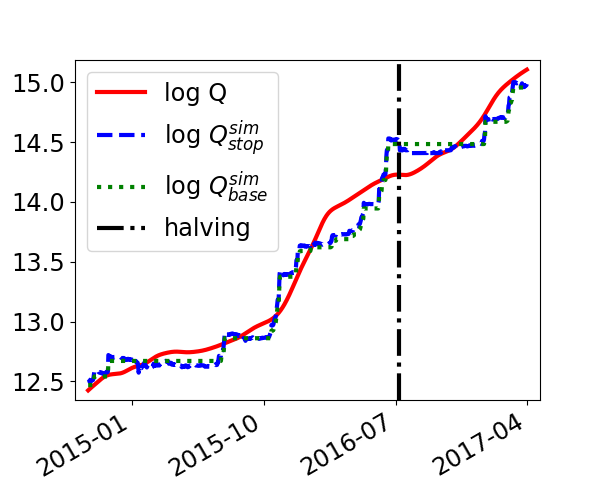
\includegraphics[scale=0.54]{images/Q_Q_sim_stop2.png}%
\end{tabular}%
\end{figure}

\emph{Predicted vs actual hashrate.---} As before, we calibrate $a$, $%
\overline{P}_0$ and $C_0$ so as to minimize the distance between the
simulated and actual hashrates. Figure \ref{fig:hashrate_variable_costs}
reports the resulting series along with the prediction of the baseline
model. As expected, the model with exit fits the data better whenever the
hashrate falls. But the improvement is rather marginal because
significant decreases were exceptional. Most of the time
the predictions of the two models coincide, thus substantiating our claim
that Assumption \ref{hyp:keep-going} is a reasonable benchmark. Adding
reversibility does not fundamentally affect the hashrate trajectory because of the very high rate
of technological progress. Scrapping is profitable for mining rigs that were purchased a few years ago,
but they have become so obsolete that they only account for a negligible share of the network hashrate.
Yet, pretending that investment is irreversible is not totally innocuous. It leads to an overestimation
of the lifetime operating costs since, in practice, all mining rigs are eventually turned off.
Having a framework that takes this option into account makes it possible to
correct the cost bias.

\subsection{Disentangling investment from operating costs}
We now explain how one can use the model with reversible investment to disentangle the price of
mining hardware from their
operating costs. The simulations reported in Figure \ref%
{fig:hashrate_variable_costs} show that miners who ignored the impact of
mothballing and scrapping decisions were nonetheless able to make
accurate predictions about the network hashrate. Thus we strengthen
Assumption \ref{hyp:miners_myopic} and consider that entrants disregard the rare
instances where the hashrate shrinks.

\begin{hyp}
\label{hyp:miners_myopic2} When forming their expectations, potential entrants
ignore the impact that mothballing and scrapping have on the network
hashrate.
\end{hyp}

Entrants who base their expectations on the premise that incumbents will
remain operational can disregard the vintage of the technology operated by other miners.
Thus Assumption \ref{hyp:miners_myopic2} implies Assumption \ref%
{hyp:miners_myopic}, although the converse is not true. Assumption \ref%
{hyp:miners_myopic2} ensures that agents expect payoffs to follow a reflected
GBM as in the baseline model. Knowing the distribution of $P$ allows us to
infer the expectations of prospective entrants. In particular, equation (\ref%
{Value_mothball}) is compatible with free entry if and only if
\begin{equation}  \label{Free_Entry_exit}
I_t \geq \int_{t}^{+\infty}e^{-r(s-t)}\left(\int_0^{\overline{P}_s}\max\left(y-C_t,0%
\right)f_{P_s|P_t}^e\left(y\right)dy\right)ds
\text{, for all t,}
\end{equation}
where $f_{P_s|P_t}^e\left(\cdot\right)$ denotes the
distribution, as anticipated by
entrants, of $P_s$ conditional on $P_t$. For brevity, we relegate the explicit expression of $%
f^e$ to the Technical Appendix \ref{app:Density_f}. Using the calibrated values
of $a$, $\overline{P}_0$
and $C_0$ to evaluate the integral
on the right-hand side of (\ref{Free_Entry_exit}) yields the investment cost $I_0$
consistent with free entry. Moreover, condition (\ref%
{Free_Entry_exit}) also places an upper bound on the overall costs of entry paid by miners.
Let $T$ denote the time it takes for the entry barrier to reach the
operating costs of entrants. Given that the entry barrier decays at
the rate of technological progress, we have $T=\log\left(\overline{P}%
_0/C_0\right)/a$. The total costs paid by miners who entered at time $0$
must necessarily be inferior to $K_0 = I_0+\int_0^TC_0e^{-rt}dt$ because
they will never find it profitable to mine after date $T$.


\begin{table}[h]
\caption{Calibration with and without Exit}
\label{table:calibration_stop}
\begin{center}
\scalebox{1}{\begin{tabular}{ll|cccc}
\hline\hline
Parameter & Interpretation & \multicolumn{2}{c}{1st period} &
\multicolumn{2}{c}{2nd period}
\\ \hline\hline
 &  & Baseline & Exit & Baseline & Exit \\
 \hline
a & Rate of TP & 1.18 & 1.15 & 0.76 & 0.76  \\
				&					         & (0.50)  & (0.44)  &  (0.12) &  (0.12) \\
$\overline{P}_0$ & Barrier & 25996 & 23858  & 5.30 & 5.05 \\
								&	                     & (25843)  & (19811)  &  (0.66) &  (0.64) \\
$K_0$ & Overall Costs of Entry & $\$5.6\times 10^6 $ & $\$4.8\times 10^6$& \$1,825 & \$1,581  \\
					 &	                          & ($1.6\times 10^7$)  & ($2.6\times 10^7$)  &  (199) &  (220) \\
$C_0$ & Daily Operating Costs & &\$2,767 & &\$0.68 \\
					 &	                          			 & & (1332)    & &   (0.38) \\
$I_0$ & Price of Mining Rig & & $\$3.1\times 10^6$ & & \$1,002  \\
					 &	                          			 & & ($2.5\times 10^7$)    & &   (444) \\
$T$ & Maximal Mining Time & &$1.87$ years & &$2.65$ years  \\
%					 &	                          			 & & (60 years)    & &   (3.6 years) \\ \hline\hline
\hline\hline
\end{tabular}}
\end{center}
\footnotesize{Note: Calibrations based on a an annual discount rate $r=10\%$.
$I_0$, $C_0$ and $K_0$ correspond to a one-Terahash per second hardware at the first day of each subperiod.
Standard errors from block bootstrap in parenthesis.}
\end{table}


Table \ref{table:calibration_stop} contains the parameter values resulting
from these computations along with their counterparts for the baseline
calibration. The overall costs of entry are lower in the model with exit
than in the baseline model. This is not surprising because miners now have a
finite horizon. Given that costs are smaller, entries happen sooner, which
translates into a lower entry barrier.

\textit{Comparing calibration to price data.---} Overall costs are made of two
components: the initial purchase of mining hardware and the daily operating costs.
Assumption \ref{hyp:miners_myopic2} allows us to disentangle
them. Their values are reported in
the fourth and fifth lines of Table \ref{table:calibration_stop}.\footnote{%
The calibrated value for $I_0$ depends on $r$ which we set equal to $0.1$.
However, our results are not very sensitive to the
choice of $r$ because the obsolescence process is so fast that miners do not
operate their hardware for a very long time. For example, $r=0.05$ yields $%
I_0=\$1033$ in the second period, while $r=0.2$ yields $I_0=\$943$.} In both subperiods
investment costs amount to around two thirds of the overall costs of entry.
Hence all seignorage income was not spent on electricity, as often argued, but
instead largely captured by mining rigs producers.

The plausibility of our calibrated parameters can be assessed by comparing them to online data on the selling price of mining hardware.
To the best of our knowledge, there is no official source for hardware characteristics and availability dates. We therefore retrieved our data from different websites, selecting those which offered the most reliable information, namely Bitcoin wiki and the Bitcoin forum. We collected data on state-of-the-art mining hardware at the time they were put on the market.\footnote{The online data and their sources are reported in the
Technical Appendix \ref{app:Price_data_2018}.} We focused on the post-2014 period because there is too much uncertainty around the
type of hardware that was used before the introduction of ASICs.

\begin{figure}[]
\caption{Calibrated vs Observed Rate of Technical Progress}
\label{fig:a_observed_simulated}\centering
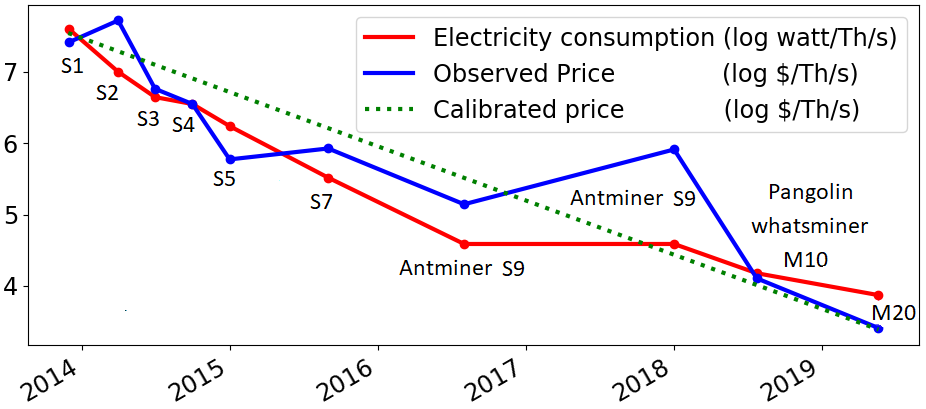
\includegraphics[scale=0.65]{images/all_sample_a_baseline}
\end{figure}

Figure \ref{fig:a_observed_simulated} reports the electricity consumption and market price of hardware, along with the price series predicted by the model.\footnote{We extrapolate the model's prediction to cover all the sample where online price data are available.}
It indicates that our calibration of the cost of investment and of the rate of technological progress are consistent with online data.
Besides supporting the parameters resulting from our calibration strategy, Figure \ref{fig:a_observed_simulated} also validates Assumption \ref{hyp:rate_TP} according to which the price of mining hardware and their energy consumption should decrease at the same rate. There is, however, a specific time window where the assumption fails to hold: Between August 2017 and February 2018, the price of mining rigs skyrocketed from around \$2,000 to \$5,200. This temporary increase was triggered by the concurrent bubble in Bitcoin price. We now explain how our model can be modified to capture this temporary deviation from the long-run trend.


\section{The 2017 Bubble and its Aftermath}
\label{sec:Bubble}

So far we have restricted our attention to pre-2018 data.
We have excluded recent observations because Bitcoin
experienced a period of trading frenzy during the winter of 2017: From three thousand dollars in
September 2017, Bitcoin exchange rate shot up to nearly twenty thousand in December, and then, dropped back to six thousand in February
2018. This bubbly episode raises a significant challenge because it led to a
structural break in the relation between the exchange rate and the network hashrate. As shown in Figure \ref{fig:hashrate_bubble}, if the
relation had remained stable, the hashrate should have been five times higher than its actual value
at the peak of the bubble.
The discrepancy between the observed hashrate and the one that would
have resulted from our frictionless model is explained by
three different factors.

First, market entry was constrained by the manufacturing capacity of ASICs producers. In May 2017, there were approximately 230,000 active
mining rigs. Between May and December 2017, the \bitcoinA /\$ exchange rate was multiplied by 12. To keep
up with this pace, approximately 2,700,000 new mining rigs would have had to be
installed within eight months only.
Such a dramatic increase was bound to
stretch the capacity of Bitmain, the main manufacturer of ASICs for
Bitcoin mining. Second, Bitmain
exercised his monopoly power and decided not to flood the market
with new hardware in order to raise their selling price. Indeed, the price
of an Antminer S9 mining rig was multiplied by three between the beginning
and the climax of the bubble, and then divided by around four during the
following crash.\footnote{%
See Technical Appendix \ref{app:Price_data_2018}.}
Third, as the bubble collapsed within a few months only,
prospective miners simply cancelled their orders or backtracked on their decision to enter the market.

We take these constraints into account by assuming that investment costs are not constant
but increasing in aggregate investment. More precisely, let $q_t$ denote
the \emph{flow of entrants} at date $t$, so that $Q_t=Q_0+\int_{0}^{t}q_sds$. The investment costs for the marginal entrant
are now given by
\begin{equation}
I\left(q_t;Q_t,A_t\right) =\frac{I_0}{A_t}\left[1+\left(\frac{q_t}{bQ_t}\right)^{\eta }\right]
\text{, for }I_0,b \in \mathbb{R}_+ \text{, and }\eta>1.
\label{I_constrained}
\end{equation}%
Congestion externalities are captured by the convex function on the right-hand side of (\ref{I_constrained}):
An increase in the flow of entrants, $q_t$, stretches manufacturing capacities, thus raising the cost
of entering the market. The parameter $\eta$ controls the convexity of the cost function.\footnote{In particular, note that
$I\left(q_t;Q_t,A_t\right)$ is isomorphic to our baseline specification when $\eta =0$.} As $\eta$ increases,
$I$ converges towards an hyperbolic function with an asymptote at $bQ_t$. Hence, one can think of $bQ_t$
as the production capacity of ASICs manufacturers, which is assumed to be proportional to the number of operational units.


\begin{figure}[t]
\caption{Model with Convex Costs}
\label{fig:hashrate_bubble}
\centering
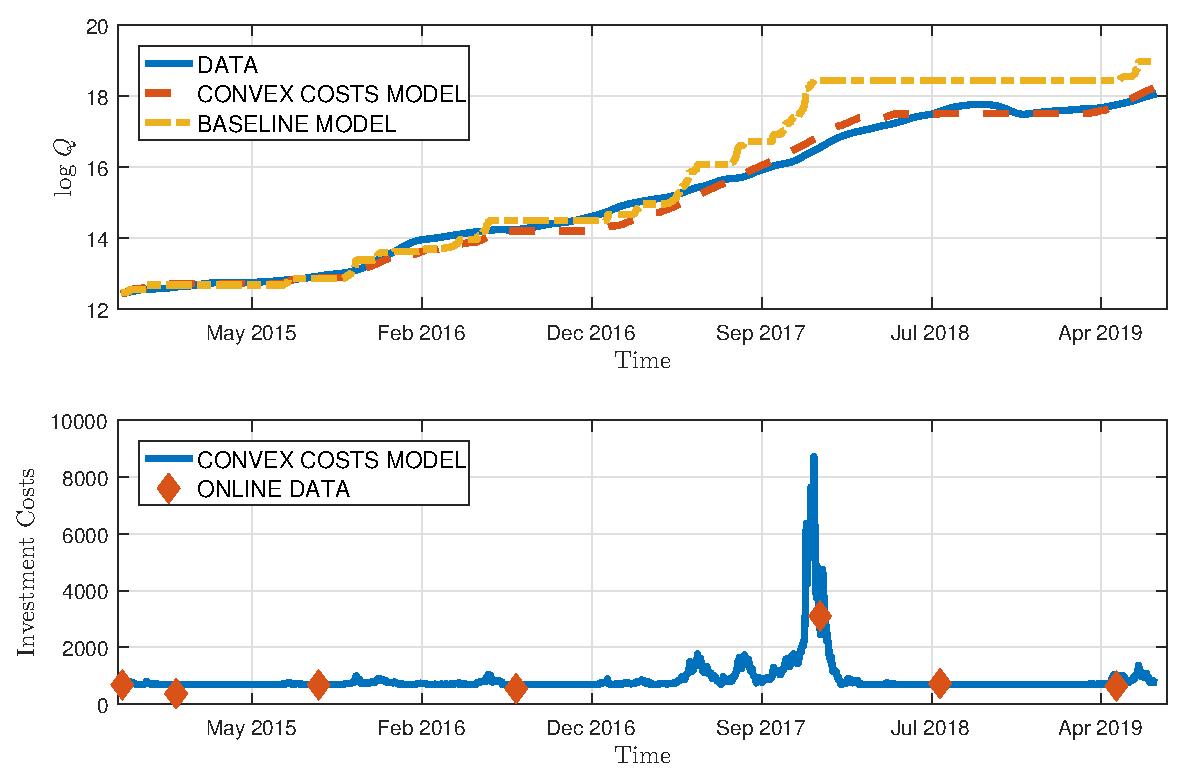
\includegraphics[scale=.775]{images/Fig_bubble_constrained.eps}
\caption*{\footnotesize{\textsc{Parameters: $r=.1$, $a=0.65$, $\eta=14.1$, $b=3$.
        \\ Note: Investment costs are multiplied by the efficiency coefficient $A_t$.}}}
\end{figure}


For brevity, the derivation of the optimal entry rule under (\ref{I_constrained}) is relegated to the Technical Appendix \ref{app:Section_convex}.
We demonstrate that, as in the baseline model, entry is a function of $P_t$ only, and that there exists
a threshold $\overline{P}_0$ such that $dQ_t=0$ whenever $P_t<\overline{P}_t=e^{-at}\overline{P}_0$.
However, $\overline{P}_t$ is not anymore
a reflecting barrier. Due to the convexity of the cost function, aggregate investment is now absolutely
continuous with respect to time.\footnote{By contrast, aggregate investment was a singular control process in the baseline model
with $dQ_t$ being (infinitesimally) positive only on a measure-zero set of time points.} Whenever $P_t>\overline{P}_t$,
an Hamilton-Jacobi-Bellman equation, whose solution can be numerically approximated, pins down the positive relationship between
$q_t$ and $P_t$.

We include the most recent observations and select, as before, the parameters that minimize the distance
between the simulated hashrate series and its empirical counterpart. We also include online price data for mining hardware
in our set of targeted moments. This enables us to identify the convexity parameter $\eta$ since
it controls the elasticity of the hardware price with respect to aggregate investment.\footnote{See
the Technical Appendix \ref{app:Section_convex} for further details on the calibration procedure.}

Figure \ref{fig:hashrate_bubble} shows that the baseline model
vastly overestimates entry during the bubbly episode, and then,
due to the irreversibility of past investment, remains well above the actual hashrate for the rest of the sample.
By contrast, calibrating the model with convex costs
enables us to match the hashrate over the full sample. The lower-panel which
reports the normalized price series, $\tilde{I}_t= A_t{I}_t$, indicates
that the simulated investment costs are also in line with the data.
As predicted by the baseline model, the investment costs
decrease at the rate of technological progress, thus generating
a flat profile when they are normalized. There is, however, a notable exception
during the height of the 2017 bubble, where the investment costs increased dramatically.
This means that the
marginal cost function (\ref{I_constrained}) is essentially flat until it nears the threshold $bQ_t$,
and starts to increase exponentially.

The calibrated parameters are reported
in the legend of Figure \ref{fig:hashrate_bubble}. The value $b=3$ implies
that the congestion externality becomes relevant solely at very high rates of investment
amounting to a twentyfold annual increase in the network hashrate. The calibration $\eta=14.1$ confirms that
the cost function is indeed extremely steep in the vicinity of $bQ_t$. This explains why the
bubble triggered a sudden burst in the cost of entry
which prevented miners to flood the market during the bubbly episode. Interestingly, our calibration
demonstrates that, even in the face of an event as extreme as Bitcoin bubble,
one does not to need to abandon the efficient market hypothesis by assuming, for instance,
that miners refrained from investing because they anticipated the incoming crash. Instead, we find that
their behaviour is explained by large variations in the price of their main input factor.


\section{Discussion}
\label{sec:Discussion}

Having established the accuracy of our framework, we use it to address the questions that motivate our analysis.
First, is Bitcoin design really generating a competitive environment for its mining industry and, if so, which actors
were able to appropriate Bitcoin's seigniorage income? Second, what forecasts
can we draw about the evolution of Bitcoin's carbon footprint?


\subsection{Revenues allocation}
\label{ssec:Oligopolistic}

\emph{Oligopolistic industry.---} Although we cannot reject the premise that miners operate under perfect competition,
our results do not prove that the premise is true either. One should be careful
when interpreting our findings because, as first established by \citeauthor{Grenadier2002} (\citeyear{Grenadier2002}),
a similar entry rule can hold even when the industry is oligopolistic. More precisely,
assume that, instead of being populated by a continuum of atomistic miners, the market is controlled by
$n$ symmetric firms. Then, provided that assumptions \ref{hyp:continuous_update}%
, \ref{hyp:keep-going}, \ref{hyp:GBM} and \ref{hyp:rate_TP} hold, there exists
a symmetric Nash equilibrium where each firm increases its mining power when $P_t$
reaches the trigger level $\overline{P}^n_t=e^{-at}\overline{P}^n_0$. As in the baseline model, $P_t$
is a GBM reflected at $\overline{P}^n_t$, where
\begin{equation}\label{Pbar_olig}
\overline{P}^n_{0}=\frac{n}{n-1}\frac{\beta (r-\alpha )}{\beta -1}K^n_{0},\text{ and } K^n_{0}=I_{0}+\frac{C_0}{r}.
\end{equation}

Given that we identify the entry barrier without relying on
the model, our calibration strategy returns the same threshold independently of whether
the industry is competitive or not. The degree of competition matters at the second stage,
when we infer the cost parameters that are consistent with the barrier.
Setting (\ref{eq:def_barrier}) equal to (\ref{Pbar_olig}), we find that
the costs in the oligopolistic and competitive models are proportional as $K^n_{t}=\left[(n-1)/n\right]K_t$.
Calibrated costs are lower when the industry is oligopolistic because firms are able to extract some rents.

We can easily construct an intuitive measure for the oligopolistic rents. First, note that the net present value of an additional unit of hashpower is equal
to $W(P_t)-K^n_{t}$, where $W(P_t) \equiv \mathbb{E}_t\left[\int_{t}^{\infty }e^{-r(s-t)}P_s ds\right]$ denotes
the expected value of discounted payoffs. The expectation operator for $P$ does not depend on the degree of competition
because it does not affect the calibrated barrier. Hence, free entry is satisfied in the baseline model if and only if $W(\overline{P}_t)=K_t$.
It follows that if we evaluate the net present value of entrants and divide it by the overall costs of entry, we find that the option premium reads\footnote{Given that the mining technology exhibits constant returns to scale at the aggregate level, the option premium is not well defined when
 $n=1$, that is when the market for mining is controlled by a monopolist.}
\begin{equation*}
\text{Option Premium}=\frac{W(\overline{P}_t)-K^n_t}{K^n_t}=\frac{1}{n-1}.
\end{equation*}
As expected, when $n$ goes to infinity, the option premium converges to zero so that free entry holds. The
option premium rapidly decreases in the number of competitors. For instance, the option premium is below $10\%$ of
expected revenues if, as suggested by \citeauthor{Alsabah} (\citeyear{Alsabah}), more than 10 mining firms are
competing. Incidentally, our model unambiguously rejects high degrees of concentration, with $n$ equal or smaller than 4, since they
would imply that the overall costs of entry are smaller than the market price of mining hardware.


\emph{Input producers.---} Since miners are not able to extract significant rents,
they channel most of their income towards the producers
of their input factors, namely hardware manufacturers and electricity suppliers.
As large mining farms are scattered around the globe (with major hubs in China, North-America, and Scandinavian countries),
evaluating their impact
requires a geographic analysis that would go well beyond
the scope of this paper. \citeauthor{Pieters} (\citeyear{Pieters}) provide
the most comprehensive survey of mining locations but, as far as we know, no study has yet used their data to assess
the effect that mining has on the revenues of local electricity providers.

By contrast, the production of ASICs was, until recently, a very concentrated activity,
with Bitmain claiming a market share of $74.5\%$ of 2017 sales revenues.
In their 2018 application proof for
an IPO on the Hong Kong Stock Exchange,\footnote{Prospectus available at http://templatelab.com/bitmain-ipo-prospectus/.
Note that Bitmain was drawing part of its revenues from proprietary mining and mining services. Yet hardware
production accounted for the bulk of Bitmain's activity, namely $90\%$ of its overall revenues.}
Bitmain indicated that it had been able to generate
$\$952.6$ million in profits out of $\$2.5$ billion in revenues, thus
reporting an healthy profit margin of $37.8\%$ in 2017. To put these numbers into perspective,
the overall seigniorage income generated by Bitcoin over the same year
was equal to $\$3.18$ billion. Hence, in line with our findings,
all seignorage income was not spent on electricity, but
instead largely captured as a monopoly rent by ASICs manufacturers.
The quasi-monopolistic position enjoyed by Bitmain
was finally contested in 2018 by the arrival of new competitors.
In particular, Halong Mining, which uses chips produced by Samsung, entered the market in March 2018,
proposing a mining rig called DragonMint 16T that was 30\% more efficient than the previous state of the art.
The entry of this new competitor triggered a dramatic drop
in the price of Bitmain's product, as can be seen in Figure \ref{fig:price_2018} in the Technical Appendix \ref{app:Price_data_2018}.


\subsection{Electricity consumption of Bitcoin}
\label{ss_Electricity}
The erosion of Bitmain's dominant position is lowering the cost of entering the mining market.
At the same time, price data indicate that Bitcoin is providing lower returns and not exhibiting as much volatility
as in the past. We also expect the
rate of technological progress to slow down and converge, in the
best case scenario, to the value predicted by Moore's law.
What will be the impact of these ongoing changes on Bitcoin's electricity consumption?
Having a structural model enables us to answer this question in a quantitative manner.



\begin{figure}[]
\caption{Impact of Parameters on Hashrate}
\label{fig:Q_comp_stats}\centering
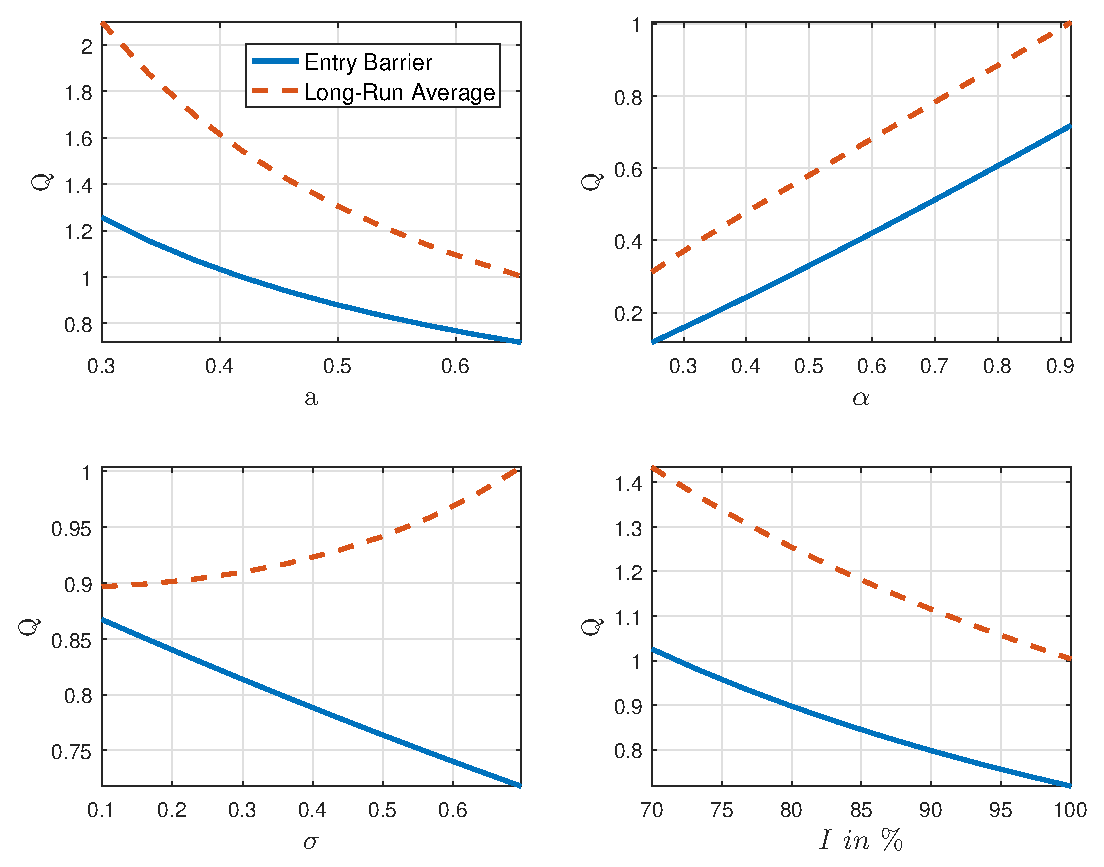
\includegraphics[scale=0.7]{images/Fig_Q_comp_stats.eps}
\end{figure}



The entry barrier fully characterizes the industry dynamics for any price trajectory.
Most of the time, however, payoffs will be below the barrier.
Thus we need to evaluate the payoffs probability distribution
in the no-entry region. Fortunately, the ergodic distribution of
reflected Brownian motions admits a closed-form solution. In order to apply it to our setting,
we first notice that the detrended payoff, $\tilde{P}_t \equiv P_tA_t$, is a GBM reflected at $\overline{P}_0$.
Then it is well known (see for instance \citeauthor{Grenadier2002} (\citeyear{Grenadier2002})) that
$\tilde{P}_t$ has a long-run stationary distribution whenever $\alpha+a>\sigma^2/2$, a condition
which is comfortably satisfied by our calibrated parameters. Using $f_{\tilde{P}}$ to denote
the ergodic density of $\tilde{P}$, we find that, for all $y\in (0,\overline{P}_0]$,
\begin{equation*}
f_{\tilde{P}}(y)=\frac{\gamma}{y}\left(\frac{y}{\overline{P}_0}\right)^{\gamma}, \text{ where } \gamma \equiv \frac{2\left(\alpha+a-\sigma^2/2\right)}{\sigma^2}.
\end{equation*}

In contrast to $\tilde{P}$, the network hashrate, $Q$, follows a non-stationary process, and thus fails to have long-run distribution.
Yet, a simple change-of-variable allows us to compute the steady-state distribution of $Q$ conditional on $R$ and $A$, as
\begin{eqnarray*}\label{eq_ergodic_Q}
f_Q(Q;R,A)&=&f_{\tilde{P}}\left(\tilde{P}(Q,R,A)\right)\frac{\partial \tilde{P}(Q,R,A)}{\partial Q}\\
& =&-\gamma Q ^{-(\gamma+1)}\left(\frac{RA}{\overline{P}_0}\right)^{\gamma}.
\end{eqnarray*}
Integrating $f_Q$ over the consistent values of $Q$ finally yields its conditional mean
\begin{equation}\label{eq_ergodic}
\mathbb{E}[Q;R,A]= \int_{\infty}^{\frac{RA}{\overline{P}_0}} Qf_Q(Q;R,A)dQ = \left(\frac{\gamma}{\gamma-1}\right)\frac{RA}{\overline{P}_0}.
\end{equation}
The electricity consumption of the network is inversely proportional to the efficiency parameter $A$. Hence
\begin{equation}\label{eq_ergodic_A}
\frac{\mathbb{E}[Q;R,A]}{A}= \left(\frac{\gamma}{\gamma-1}\right)\frac{R}{\overline{P}_0}
\end{equation}
is the best guess one can make about the long-run energy requirements of Bitcoin. Since (\ref{eq_ergodic_A}) is linearly increasing
in block rewards, our model confirms the widely held belief that halvings will lower Bitcoin's electricity consumption.
Our contribution consists in characterizing the slope of the relation between $R$ and
$Q$. Figure \ref{fig:Q_comp_stats} reports the impact of the parameters on
the conditional expectation of $Q$, as well as on its value at the entry barrier.
For readability, we set $R$ and $A$ equal to one. We also normalize to one the average value
of $Q$ generated by the calibrated parameters.
Hence, all changes can be interpreted as percentage deviations from the calibrated model.

First we lower $a$ from its calibrated value
to the one consistent with Moore's law. The results reported in the north-west panel
of Figure \ref{fig:Q_comp_stats} show that a decrease in the rate of technological progress significantly raises the
average hashrate. As hardware becomes obsolete at a lower pace, miners are able to devote
a greater share of their income to operating costs.
Not surprisingly, the growth rate of block rewards, $\alpha$, has a positive impact on the level
of investment as more miners find it attractive to enter the market. The impact of the volatility
coefficient, $\sigma$, is more intriguing since it has opposite effects on the entry barrier and
average hashrate. When $\sigma$ increases, miners are more reluctant to enter the market because
they anticipate that large negative shocks are more likely to leave them burdened with excess mining power.\footnote{Note that $Q$ and $P$ are
negatively correlated, hence a decrease in the
value of $Q$ at the entry barrier is equivalent to an increase in the entry barrier $\overline{P}$.}
This added dispersion is what drives apart the conditional expectation
and entry barrier in the south-west panel of Figure \ref{fig:Q_comp_stats}. As these opposite effects partially compensate
each other, $\sigma$ has a positive but relatively modest effect on the average hashrate.
Finally, we report the impact of a decrease in the selling price of mining hardware $I$.
We use Bitmain's 2017 profit margin of around $30 \% $ as an upper-bound on the price correction.
When hardware become cheaper, miners enter the market in greater numbers and
devote more of their resources to electricity consumption.

Finally, our framework predicts that energy requirements are increasing in the degree of competition among miners.
Let $\mathbb{E}^n[Q;R,A]$ denote the conditional expectation of $Q$ when the mining market is oligopolistic with $n$ symmetric firms.
Reinserting (\ref{Pbar_olig}) into (\ref{eq_ergodic}), we find that an increase in the number of competing firms $n$ raises the network hashrate since $\mathbb{E}^n[Q;R,A]=\left(1-1/n\right)\mathbb{E}[Q;R,A]$.
Given that normative studies conclude that Bitcoin hashrate is too high (see for instance \citeauthor{Huberman} (\citeyear{Huberman})),
encouraging concentration in the mining market is likely to increase welfare.

What lessons can be drawn from these experiments regarding the future of
Bitcoin's electricity consumption? The increased competition between
hardware producers and, most notably, the decrease in the rate of technological
progress will worsen Bitcoin's carbon footprint. For these trends to be contained,
Bitcoin price will have to stabilize, thus suggesting that the carbon footprint
may eventually place a hard cap on the price of Bitcoin.

\section{Conclusion}

\label{sec:conclusion}


One of the most enticing promise of Blockchains
is their ability to support the maintenance of their infrastructure
through a decentralized network. Decentralization
has received a lot of attention, becoming a byword for Blockchains and their
capacity to dislodge traditional intermediaries. Yet, the extent to which Blockchains
truly achieve decentralization remains open to debate. We address this issue
by assessing whether Bitcoin is indeed able to
create a competitive market for intermediaries. To the best of our knowledge, our paper
is the first to use a structural model to answer this question, and our conclusion is mostly positive:
the confirmation and immutability of Bitcoin transactions is
guaranteed by a market that operates under competitive conditions.

Our findings should be of interest beyond the community of economists
working on Bitcoin and Blockchains. They demonstrate that Bitcoin
is a remarkable example of mechanism design on a wide scale. Bitcoin protocol encodes several features that are
rarely observed. Agents mostly face
aggregate uncertainty. They operate a common technology which exhibits constant
returns to scale at the micro-level, and earn revenues that are decreasing
in aggregate capacity. All these characteristics make the mining market
a perfect laboratory for models of industry dynamics, all the more so since data are exhaustive, clean and
publicly available. In particular, we show how one can observe the
entry barrier using industry-level data only. As far as we are aware, no other industry
has yet been used to construct such a direct measure,
and it is therefore reassuring that the canonical model of industry dynamics
convincingly replicates the evolution of mining capacity.

Our analysis also has normative implications that go well beyond the scope of model testing.
It supports the view that Blockchains provide
a meaningful alternative for the design of online platforms and marketplaces.
The surge of the digital economy is raising ever more pressing concerns about the predatory behavior
of platform owners. We find that their market power could be mitigated through the
introduction of tokens, and the creation of markets for infrastructure maintenance.
Scores of companies are trying to emulate Bitcoin design across various sectors of the
digital economy. Our results indicate that, when properly harvested, market forces and price signals
are indeed able to coordinate agents, thus avoiding the emergence of a monopolistic owner
in favor of a market allocation of revenues among the many stakeholders.

Finally, we believe that our findings will be of
interest to Bitcoin practitioners since our model
provides a forecasting tool for investors
willing to enter the mining industry. From a practical standpoint, it has three
main implications. First, the hashrate of the network is closely related to
the exchange rate and, in the event of a significant market crash, the
hashrate barely moves in the short run due to the irreversibility of past
investments. This is good news for the security of Bitcoin transactions but
bad news for their carbon footprint. Second, around two thirds of all
seigniorage income was not dissipated in electricity consumption, as often
argued, but was instead spent on mining hardware. Third, we expect the energy
efficiency of the network to deteriorate if the rate of technological
progress decelerates from the high pace it has experienced so far.

Although our model is fairly accurate in the medium to long run, it
assumes that the environment is stationary. Since this restriction is hard to maintain
over a long horizon, a promising direction for further research would be to embed our framework
into a non-stationary environment, and allow agents to update their priors. Future
research should also strive to improve our granular understanding of the mining industry
by building on the growing amount of geographical data.
Finally, our modeling strategy is likely to apply to other cryptocurrencies.
Taking into account the ability of miners to concurrently mine multiple cryptocurrencies
would bring us closer to a proper understanding of the ecosystem built around Bitcoin.


\nocite{*}
\bibliographystyle{apalike}
\bibliography{biblioWP}

\newpage

\section{Appendix}

\label{sec:appendix}

\subsection{Proof of Propositions}

\paragraph{Proof of Proposition \protect\ref{prop:industry-eq}}

\label{app:preuve_closed_form}

Let $W\left(P_t,\overline{P}_t,A_t\right)\equiv V\left(P_t,t\right)+C_t/r$
denote the value of an entrant net of operating costs as a function of the
payoff $P_t$, the entry barrier $\overline{P}_t$ and the efficiency of the
technology $A_t$. Assumption \ref{hyp:rate_TP} requires that $dA_t=-aA_tdt$.
Assumptions \ref{hyp:continuous_update} and \ref{hyp:GBM} imply that $%
dP_t=P_t\left(\alpha dt +\sigma dZ_t\right)$ whenever $P_t< \overline{P}_t$
because $Q_t$ remains constant in that region of the payoff space. Finally,
the law-of-motion of the entry barrier $\overline{P}_t$ is endogenous, and it
is precisely the aim of this proof to show that the market for mining
satisfies the equilibrium requirements stated in Definition \ref%
{def:industry-eq} when $\overline{P}_t$ decreases at the rate of
technological progress. Thus we conjecture that $\overline{P}_t=\overline{P}%
_0/A_t$, with $\overline{P}_0$ as in Proposition \ref{def:industry-eq}, and
proceed to show that it is indeed optimal for entrants to wait until $P_t=%
\overline{P}_t$.

Having specified the law of motion of the three state variables allows us to
use Ito's Lemma to derive the Hamilton-Jacobi-Bellman equation satisfied by
the value function
\begin{eqnarray*}  \label{eq:equa_diff}
rW\left(P_t,\overline{P}_t,A_t\right)&=&P_t+\alpha P_tW_1\left(P_t,\overline{%
P}_t,A_t\right)-a\overline{P}_tW_2\left(P_t,\overline{P}_t,A_t%
\right)+aA_tW_3\left(P_t,\overline{P}_t,A_t\right) \\
&&+\frac{\sigma^2}{2}P_t^2W_{11}\left(P_t,\overline{P}_t,A_t\right),
\end{eqnarray*}
when $P_t < \overline{P}_t$. Assume that $\alpha \neq r$,\footnote{%
As $r$ tends to $\alpha$, $\overline{P}_0$ converges to $\left(I_0+\frac{C_0%
}{\alpha}\right)\left(\alpha+a+\sigma^2/2\right)$ and $W\left(P_t,\overline{P%
}_t,A_t\right)$ tends to $\frac{I_0+\frac{C_0}{\alpha}}{A_t}\left(\frac{P_t}{%
\overline{P}_t}\right)\left[1-\log\left(\frac{P_t}{\overline{P}_t}\right)%
\right]$.} then the general solution of the Hamilton-Jacobi-Bellman equation
reads
\begin{equation*}
W\left(P_t,\overline{P}_t,A_t\right)=\frac{P_t}{r-\alpha}+\frac{D_1}{A_t}%
\left(\frac{P_t}{\overline{P}_t}\right)^{\beta_1}+\frac{D_2}{A_t}\left(\frac{%
P_t}{\overline{P}_t}\right)^{\beta_2},
\end{equation*}
where $D_1$ and $D_2$ are constants whose values will be chosen so as to
match some boundary conditions, while $\beta_1$ and $\beta_2$ are the two
roots of the following quadratic equation
\begin{equation*}
\mathcal{Q}(\beta)\equiv\frac{\sigma^2}{2}\beta(\beta-1)+(\alpha+a)%
\beta-a-r=0.
\end{equation*}
Since $\mathcal{Q}(0)=-a-r<0$ and the coefficient associated to the second order term
is strictly positive, we know that one root, $\beta_1$ for instance, is
strictly positive while the other root, $\beta_2$, is strictly negative.

%Instead of directly using the boundary conditions to pin down the constants,
%we first note that $W$ is log-linear in $A_t$ since
%\begin{equation*}
%w\left(\tilde{P}_t\right)\equiv\frac{\tilde{P}_t}{r-\alpha} +D_1\left(\frac{%
%\tilde{P}_t}{\overline{P}_0}\right)^{\beta_1}+D_2\left(\frac{\tilde{P}_t}{%
%\overline{P}_0}\right)^{\beta_2}
%\end{equation*}
%satisfies
%\begin{equation}
%w\left(\tilde{P}_t\right) = A_tW\left(P_t,\overline{P}_t,A_t\right) \text{
%when } \tilde{P}_t\equiv{P}_tA_t.  \label{W_norm}
%\end{equation}

The function $W$ has to satisfy the following three boundary conditions.
First, since $P_t=0$ is an absorbing state, we must have $W(0,%
\overline{P}_t,A_t)=0$. This implies that $D_2=0$, as otherwise the value
function would diverge to either minus or plus infinity when $P$ goes to
zero. Second, the left continuity of the value function at the entry
threshold $\overline{P}_t$ implies that there can be no arbitrage
opportunity solely if the value function is flat at the contact point. This
requirement, known as the smooth-pasting condition, is satisfied when $%
W_1\left(\overline{P}_t,\overline{P}_t,A_t\right)=0$, i.e. when $D_1=-\frac{%
\overline{P}_0}{\beta_1(r-\alpha)}$. Finally, the entry barrier is pinned
down by the free entry condition $W\left(\overline{P}_t,\overline{P}%
_t,A_t\right)=I_t+C_t/r$, %Equation (\ref{W_norm}) shows that
%free entry holds at all dates if $w\left(\overline{P}_0\right)=I_0+C_0/r$,
%i.e.
which implies that $\overline{P}_0=\left(I_0+C_0/r\right)\frac{(r-\alpha)\beta_1}{%
\beta_1-1} $.\footnote{%
Alternatively, we could have solved the planner's problem and used the
"super contact" condition $W_{11}\left(\overline{P}_t,\overline{P}%
_t,A_t\right)=0$.} Thus we have found a solution which satisfies all the
requirements laid-out in Definition \ref{def:industry-eq} for the existence
of a competitive equilibrium.

\paragraph{Proof of Proposition \protect\ref{prop:industry-eq-variable-costs}%
}

We proceed as in the proof of Proposition \ref{prop:industry-eq}. We assume
that $\overline{P}_t=\overline{P}_0/A_t$, for some $\overline{P}_0$, and
show that it is indeed optimal for miners to enter the race when $P_t=%
\overline{P}_t$. The value function of an active miner entered at time $\tau$
reads $W\left(P_t,\overline{P}_t,C_\tau\right)=\int_t^{+\infty}\left(\int_0^{%
\overline{P}_s}\max(x-C_\tau,0)f_{P_s|P_t}^e(x)dx\right)e^{-r(s-t)}ds$,
where $f_{P_s|P_t}^e$ denotes the density of the payoff variable at time $s$
as anticipated by entrants at time $t$. Under the equilibrium rule, the
barrier $(\overline{P}_s)_{s\geq t}$ is deterministic. This is why we do not
account for the dependency on the whole future trajectory of the barrier
when defining $W$. We only need to show that $W\left(\overline{P}_t,%
\overline{P}_t,C_t\right)=W\left(\overline{P}_0,\overline{P}_0,C_0\right)/A_t
$ because then the condition $W\left(\overline{P}_t,\overline{P}%
_t,C_t\right)=I_t=I_0/A_t$ will be met for all $t$ whenever $\overline{P}_0$
is chosen such that $W\left(\overline{P}_0,\overline{P}_0,C_0\right)=I_0$.

According to Assumption \ref{hyp:miners_myopic}, potential entrants make
their entry decisions based on $P_t$ and $\overline{P}_t$ only. Multiplying
the two variables by the rate of technological progress, this implies
that potential entrants make their entry decisions based on $A_tP_t$ and $%
\overline{P}_0$ only. In this detrended space, the barrier is flat. Hence,
under the conjectured rule for entry, the process $A_tP_t$ anticipated by
potential entrants is Time-Homogeneous Markov, meaning that for all t, s, $\delta >0$, we have: $%
f_{A_tP_t|A_sP_s}^e(y)=f_{A_{t-\delta}P_{t-\delta}|A_{s-\delta}P_{s-\delta}}^e(y)$. Reinserting
this equality into the definition of $W$, we find that
\begin{align*}
W\left(\overline{P}_t,\overline{P}_t,C_t\right)&=\int_{t}^{+\infty}\left(%
\int_0^{\overline{P}_s}\max\left(x-C_t,0\right)f_{P_s|P_t=\overline{P}%
_t}^e(x)dx\right)e^{-r(s-t)}ds &  \\
&=\int_{0}^{+\infty}\left(\int_0^{\frac{\overline{P}_u}{A_t}%
}\max\left(x-C_t,0\right)f_{P_{u+t}|P_t=\overline{P}_t}^e(x)dx%
\right)e^{-ru}du &  \\
&=\int_{0}^{+\infty}\left(\int_0^{\overline{P}_u}\frac{1}{A_t}\max\left(%
\frac{y}{A_t}-\frac{C_0}{A_t},0\right)f_{P_{u+t}|P_t=\overline{P}_t}^e\left(%
\frac{y}{A_t}\right)dy\right)e^{-ru}du &  \\
&=\frac{1}{A_t}\int_{0}^{+\infty}\left(\int_0^{\overline{P}%
_u}\max\left(y-C_0,0\right)f_{P_{u+t}A_t|A_tP_t=\overline{P}%
_0}^e\left(y\right)dy\right)e^{-ru}du &  \\
&=\frac{1}{A_t}\int_{0}^{+\infty}\left(\int_0^{\overline{P}%
_u}\max\left(y-C_0,0\right)f_{P_u|P_0=\overline{P}_0}^e\left(y\right)dy%
\right)e^{-ru}du &  \\
&=\frac{W\left(\overline{P}_0,\overline{P}_0,C_0\right)}{A_t}. &
\end{align*}
The second equality follows from $u = s-t$ and replacing $\overline{P}_{u+t}$
by $\overline{P}_u/A_t$. The third and fourth equalities use the change of
variable $y=A_tx$. The fifth equality is a direct consequence of the
Time-Homogeneous Markov property of $A_tP_t$. The last equality holds by
definition, proving that free entry is indeed satisfied when $\overline{P}%
_t$ decays at the rate of technological progress.


\newpage



\appendix
\begin{center}
\Large{\textsc{TECHNICAL APPENDIX}}
\end{center}

\section{Derivation of equations (\ref{eq:vrai_faux_P}) and (\ref{eq:V})}
\label{app:Derivation_payoff}

Let $D$ denote the difficulty of the hashing problem, so that every computed
hash will lead to a valid block with probability $1/D$. Consider a machine
that performs on average a hash per period. Let $\left( T_{n},n\geq 0\right) $
be a strictly increasing sequence of random variables--$%
T_{0}=0<T_{1}<...<T_{n}$, which measures the dates at which the machine has
generated a valid block. To keeps track of the number of mined blocks
within $\left[ 0,t\right] $, we also introduce the counting process
associated with $T_{n}$%
\begin{equation*}
N_{t}\equiv \sum_{n\geq 1}\mathbf{1}_{\left\{ T_{n}\leq t\right\} },\ \text{%
and }N_{0}=0.
\end{equation*}

The Poisson distribution is obtained breaking up each period into tiny
intervals of size $\delta $, so that there is a very large number, $%
n=1/\delta $, of subintervals in each period. The probability that the
machine computes a hash in each subinterval is proportional to their
length $\delta$. Hence, the probability that the machine generates a block in
each subinterval is equal to $ \delta/D$, and the machine will find $k$
valid blocks in $\left[ 0,t\right] $ with probability
\begin{equation*}
\mathbb{P}\left( \left. N_{t}=k\right\vert \mathcal{F}_{0}\right) =\binom{nt%
}{k}\left( \frac{\delta }{D}\right) ^{k}\left( 1-\frac{\delta }{D}\right)
^{nt-k},
\end{equation*}%
where $\mathcal{F}_{t}=\sigma \left( N_{s},s\leq t\right) $ is the
filtration generated by $N_{t}$. Replacing $n=1/\delta $ and $\lambda \left(
x,D\right) \equiv x/D$ into the previous equation, we finally find that, when
$\delta $ converges to zero,%
\begin{eqnarray*}
\mathbb{P}\left( \left. N_{t}=k\right\vert \mathcal{F}_{0}\right)  &=&\binom{%
t/\delta }{k}\left( \lambda \left( 1,D\right) \delta \right) ^{k}(1-\lambda
\left( 1,D\right) \delta )^{t/\delta -k} \\
&\approx &\frac{\left( t/\delta \right) ^{k}}{k!}\left( \lambda \left(
1,D\right) \delta \right) ^{k}(1-\lambda \left( 1,D\right) \delta
)^{t/\delta } \\
&=&\frac{\left( \lambda \left( 1,D\right) t\right) ^{k}}{k!}(1-\lambda
\left( 1,D\right) \delta )^{t/\delta } \\
&\approx &\frac{\left( \lambda \left( 1,D\right) t\right) ^{k}}{k!}%
e^{-\lambda \left( 1,D\right) t}.
\end{eqnarray*}%
Note that considering $h$ units of hashpower simply rescale the Poisson
arrival rate.\ The memory-less property of the hashing problem implies\ that
the number of computed hashes per subintervals is equal to $h/D$ instead of $%
1/D.\ $Following the sames steps as before, one finds that the Poisson
arrival rate $\lambda \left( h,D\right) =h/D.$

Having established that the probability of finding a block is captured by a
Poisson process, we now derive the flow revenues of miners.\ It is given by
a compound process whose jumps of random sizes are proportional to the
exchange rate $R$.\ Hence, the revenues generated in $\left[ 0,t%
\right] $ read%
\begin{equation*}
\Pi _{t}=\sum_{i=1}^{N_{t}}R_{T_{i}}=\int_{0}^{t}R_{s}dN_{s}.
\end{equation*}
Fix a $t$ small enough such that the expectation of $\Pi _{t}$ is finite.\
Then we have%
\begin{eqnarray*}
\mathbb{E}_{0}\left[ \Pi _{t}\right]  &=&\mathbb{E}_{0}\left[
\int_{0}^{t}R_{s}dN_{s}\right]  \\
&=&\mathbb{E}_{0}\left[ \int_{0}^{t}R_{s}\lambda \left( 1,D_{s}\right) ds%
\right] -\overset{=0}{\overbrace{\mathbb{E}_{0}\left[ \int_{0}^{t}R_{s}%
\left( \lambda \left( 1,D_{s}\right) ds-dN_{s}\right) \right] }} \\
&=&\mathbb{E}_{0}\left[ \int_{0}^{t}\frac{R_{s}}{D_{s}}ds%
\right] ,
\end{eqnarray*}%
where the third equality follows from the fact that the compensated process $%
M_{t}\equiv N_{t}-\int_{0}^{t}\lambda \left( 1,D_{s}\right) ds\ $is a
martingale--see \citeauthor{Jeanblanc} (\citeyear{Jeanblanc}), and that $R_{t}$ and $M_{t}$ are independent.\ Finally, letting $%
t$ converge to $0$, we find that the flow payoff of the miner is indeed
equal to $P_{t}=R_{t}\lambda \left( 1,D_{t}\right) =R_{t}/D_{t}$, as stated in eq. (\ref{eq:vrai_faux_P}).

\bigskip

The value function of miners is by definition equal to%
\begin{eqnarray*}
V\left( R_{t},\tau \right)  &=&\mathbb{E}_{t}\left[ \sum_{i:T_{i}\geq
t}e^{-r\left( T_{i}-t\right) }R_{T_{i}}\right] -\int_{t}^{\infty
}e^{-r\left( s-t\right) }C_{\tau }ds \\
&=&\mathbb{E}_{t}\left[ \int_{t}^{\infty }e^{-r\left( s-t\right) }R_{s}dN_{s}%
\right] -\frac{C_{\tau}}{r}.
\end{eqnarray*}%
As before, we can use the martingale property of the compensated process $%
M_{t}$ to express the expectation as a function of the payoff process.
Following similar steps, we find that%
\begin{eqnarray*}
V\left( R_{t},\tau \right)+\frac{C_{\tau}}{r}  &=&\mathbb{E}_{t}\left[
\int_{t}^{\infty }e^{-r\left( s-t\right) }R_{s}dN_{s}\right]  \\
&=&\mathbb{E}_{t}\left[ \int_{t}^{\infty }e^{-r\left( s-t\right)
}R_{s}\lambda \left( 1,D_{s}\right) ds\right] -\overset{=0}{\overbrace{%
\mathbb{E}_{t}\left[ \int_{t}^{\infty }e^{-r\left( s-t\right) }R_{s}\left(
\lambda \left( 1,D_{s}\right) ds-dN_{s}\right) \right] }} \\
&=&\mathbb{E}_{t}\left[ \int_{t}^{\infty }e^{-r\left( s-t\right) }P_{s}ds%
\right] ,
\end{eqnarray*}%
as stated in eq. (\ref{eq:V}). Note that since we cannot arbitrarily choose
the upper-bound of the integral, we also to need to make sure that the
expectation is bounded. But this will hold true in equilibrium, as
otherwise the investment process would violate free entry.

\bigskip

\section{Entry rule during the first period}
\label{app:1st_period}

Figure \ref{fig:payoffs_p1} displays the simulated and observed payoffs series for our first period, along with the Bitcoin/US Dollar exchange rate.
As explained in the main text, the baseline model fails to match the payoff series when the exchange rate suddenly increases. This is particularly
noticeable at the beginning of the first period. Yet the model with time-to-build manages to correct this shortcoming and fir the data over the whole sample.

\bigskip

\section{Exchange rate data for Bitcoin}
\label{Bitcoin price data}

There is no single Bitcoin price as each exchange has its own exchange rate, which can sometimes be significantly different from another exchange's. The data we use in the article comes from the blockchain information website Coindesk.
To make sure that we use high quality data, we compare them with the exchange rate series constructed by \citeauthor{Biais2018} (\citeyear{Biais2018}). They rely on the Kaiko dataset,
and use all transaction prices from 17 major exchanges: Bitfinnex, bitFlyer, Bitstamp, Bittrex, BTCe, BTCChina, CEX.IO, Coinbase-GDAX, Gatecoin, Gemini, hitBTC, Huobi,
itBit, Kraken, Mt.Gox, OKCoin and Quoine. Figure \ref{fig:Kaiko_exchange_rate} plots the two series and shows that they are almost always superimposed.


\begin{figure}[H]
\caption{Simulated vs. Observed Payoffs}
\label{fig:payoffs_p1}\centering
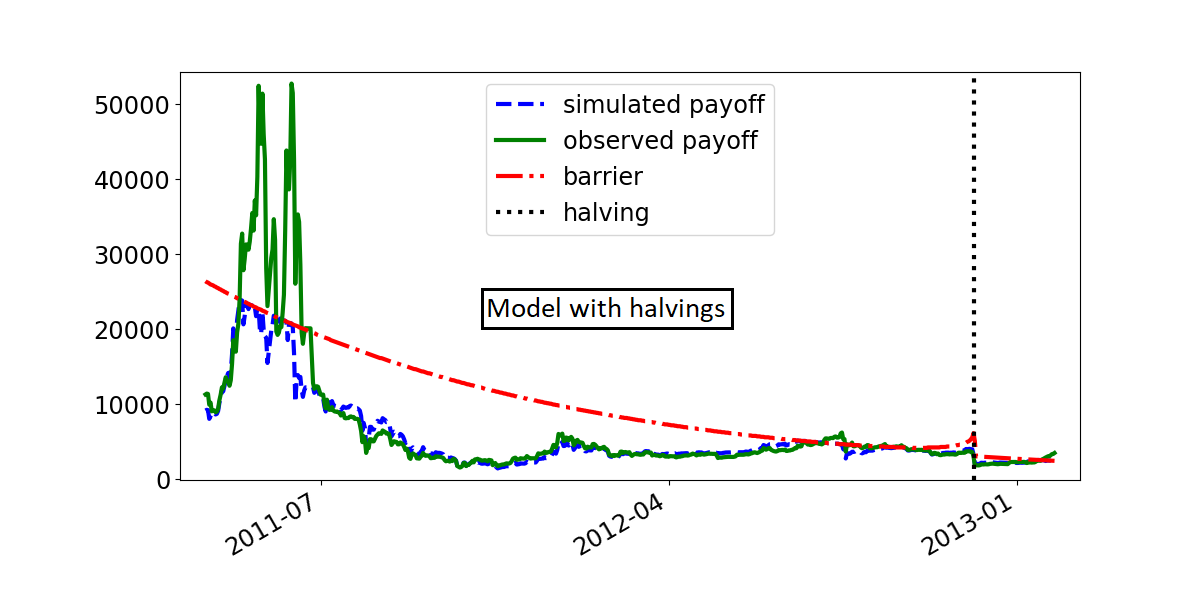
\includegraphics[scale=0.48]{images/P_P_sim_hf_1_wide.png}
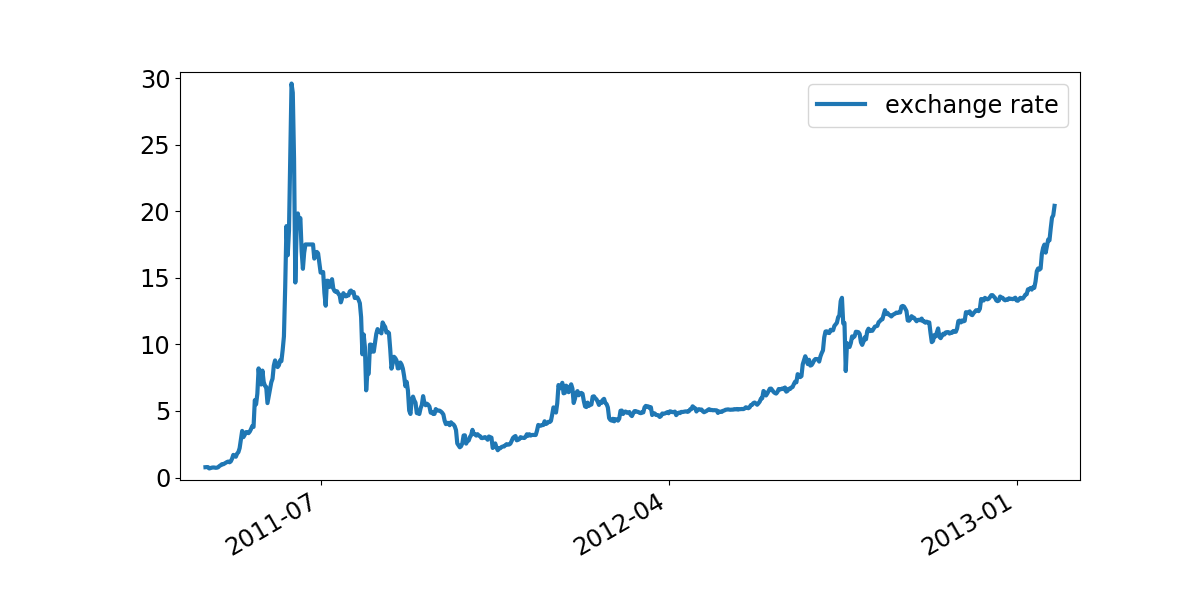
\includegraphics[scale=0.50]{images/cours1_wide.png}
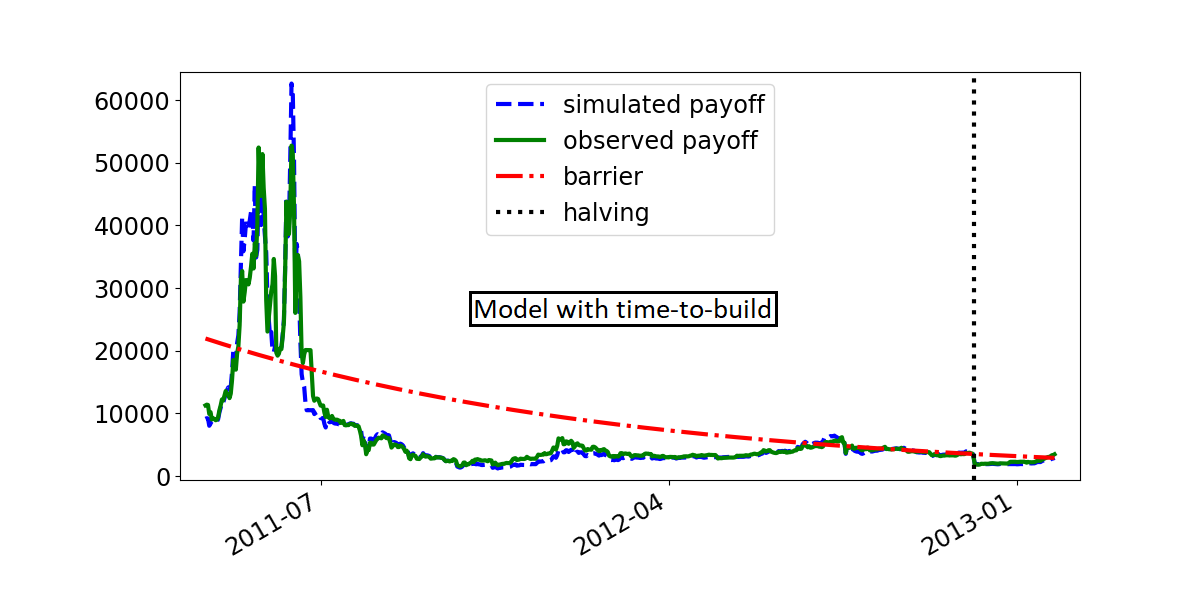
\includegraphics[scale=0.48]{images/P_P_sim_delay_1_wide.png}
\end{figure}


\begin{figure}[H]
\centering
\caption{Comparison of Exchange Rate Data}
\label{fig:Kaiko_exchange_rate}
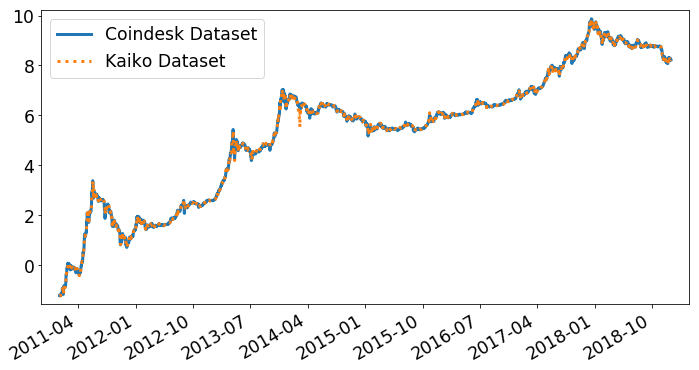
\includegraphics[scale=0.55]{images/Kaiko_exchange_rate}
\end{figure}



\section{Block generation rate}

\label{app:test_cont_update}


According to Assumption \ref{hyp:continuous_update}, the expected value of the block generation rate would
always be equal to 10 minutes. Hence it implies that the daily number of generated blocks
should not be statistically different from 144. Figure \ref{fig:N} plots the
daily number of blocks found along with the two 95\% confidence bounds. For our
periods of interest, the results are satisfying except for the beginning
of the first period. According to this graph, it is sensible not to consider
the interval separating our two periods of study. Then, due to the introduction of ASICs, technological
progress was so fast that the hashrate significantly exceeded the target of one block every ten
minutes.


\begin{figure}[H]
\caption{Number of Blocks Found per Day}
\label{fig:N}\centering
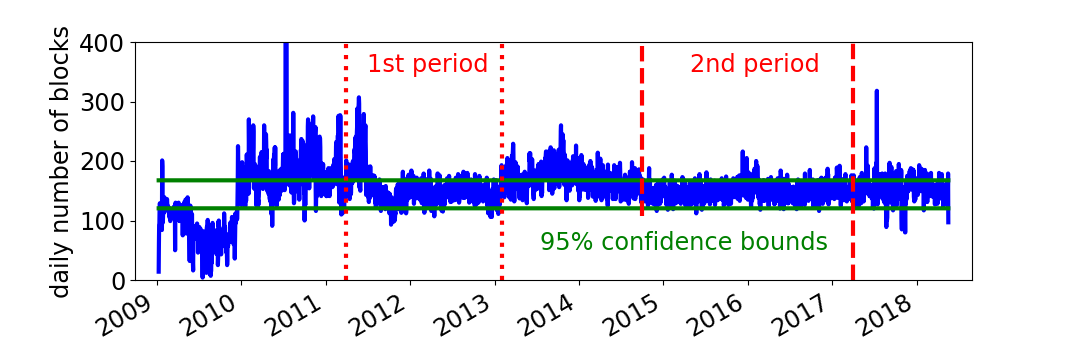
\includegraphics[scale=0.5]{images/N.png}
\caption*{Note: The number of blocks found per day has been retrieved from coindesk.com.}
\end{figure}


\section{Law-of-motion of block rewards }

\label{app:test_GBM}

The GBM assumption implies that the log-increments of block
reward should be both independent and normally distributed.
For all $t \geq 0$, we have $R_t = R_0 e^{\left(\alpha-\frac{\sigma^2}{2}\right)t+\sigma Z_t}$, where $(Z_t)_t\geq 0$ is a standard Brownian motion.
Hence we get
\begin{align*}
%\frac{R_{t+1}}{R_t}&=e^{\alpha-\frac{\sigma^2}{2} + \sigma \left(Z_{t+1}-Z_t\right)},\\
\log\left(\frac{R_{t+1}}{R_t}\right)&=\left(\alpha-\frac{\sigma^2}{2}\right) + \sigma \left(Z_{t+1}-Z_t\right).
\end{align*}
According to the definition of Brownian motions, $Z_{t+1}-Z_t$ should follow a $\mathcal{N}(0,1)$ distribution, independent from $Z_{s+1}-Z_s$ for all $s\neq t$.
Letting $\mu = \alpha-\sigma^2/2$, we see that the log-increments, $\log\left(\frac{R_{t+1}}{R_t}\right)$, are i.i.d and follow a $\mathcal{N}(\mu,\sigma^2)$ distribution.

Figure \ref{fig:test_GMB} compares the nonparametrically estimated density of log-increments
with their normal density estimated by maximum likelihood under the GBM assumption.
It show that if we exclude tail events by discarding
the 5\% most extreme increments on each side, the empirical distribution is well approximated by a normal distribution.
Hence although log-increments are  most of the time normally distributed, they exhibit fat-tails as often observed with financial data.

\begin{figure}[H]
\caption{Normality of Log-Increments}
\label{fig:test_GMB}\centering
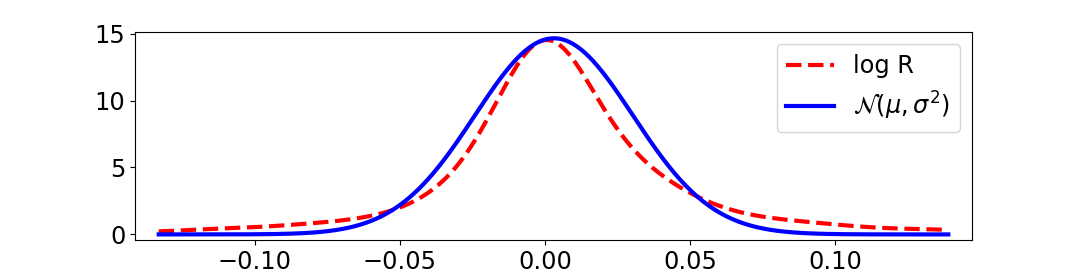
\includegraphics[scale=0.62]{images/test_brownien.png}
\caption*{Note: Estimation of log-increments excluding tail events.}
\end{figure}


As for the independence property, Figure \ref{fig:indep_returns} shows that
log-increments are not linearly autocorrelated. We obtain similar
results composing the log-increments with non-linear functions. However, statistical tests
indicate that the variance of the block rewards does not remain constant over time, and goes instead through periods of high
and low volatility. Although the issue is strongly alleviated by our division of the sample
into two subperiods, it suggests that a more realistic specification should
allow the variance coefficient $\sigma$ to vary over time. We leave this
extension to further research because it would render the entry barrier state dependent, and
thus greatly complicates the characterization of the equilibrium.


\begin{figure}[H]
\caption{Independence of Log-Increments}
\label{fig:indep_returns}\centering
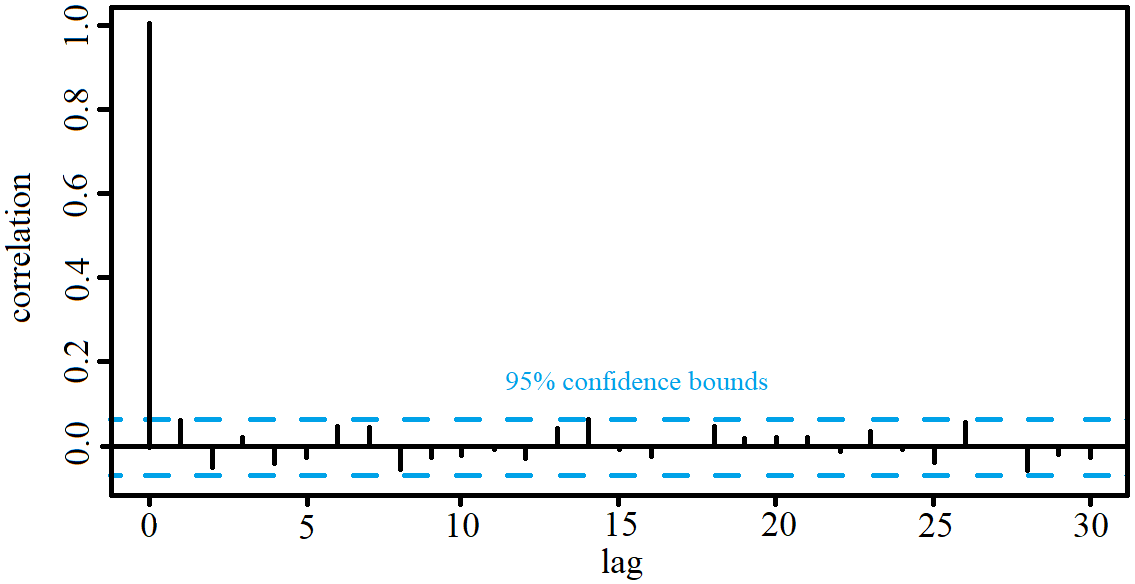
\includegraphics[scale=0.425]{images/autocorrelogramme} \flushleft
\caption*{Note: This autocorrelogram has been obtained using the second
period log-increments.}
\end{figure}


\section{Estimation of Q}

\label{app:estimation_Q}

The network's hashrate $(Q_t)_{t\geq 0}$ is not observable but can be estimated using a two-step
procedure. First, for each day $t$, let $\hat{Q}_t \equiv N_t/\tilde{\Pi}_t$%
, where $N_t$ is the number of blocks found for day $t$ and $\tilde{\Pi_t}$
is the probability to find a valid block with a single hash. Both are
directly observable in the blockchain. Since $N_t$ follows the binomial distribution with parameters $Q_t$ and $\tilde{\Pi}_t$, $\hat{Q}_t$ is a very natural estimator of the daily
hashrate. This estimator is non biased and it can easily be shown that it is
asymptotically equivalent to the maximum likelihood estimator. Given that
there is a lot of variation across daily estimates, we smooth this
new time series using a local linear regression. Figure \ref{fig:Q} shows that we
are not losing much information performing a local linear regression over $%
\hat{Q}$.

%\begin{table}[!h]
%\begin{tabular}{cc}
%\includegraphics[scale=0.5]{comparaison_Q_Q_chap_1.png} & %
%\includegraphics[scale=0.5]{comparaison_Q_Q_chap_2.png} \\
%&
%\end{tabular}%
%\caption{Estimation of $Q$}\label{fig:Q}
%\end{table}



The two green curves are confidence bounds for the first step estimation if
the true $(log\left(Q\right)_t)_{t\geq 0}$ were the red curve (the second
step estimate). If the erratic variations of the first step estimation
captured not only the first step estimation variance, but also some real
variations of the hashrate not captured by the second step estimation, then
its variance should be bigger than the one resulting from the first step
estimation error only. Thus it should cross the green bounds much more often
than $5\%$ of the time, which does not happen in our data. For the sake of
clarity, we do not show the whole series but the test works very well over
the whole period.

\begin{figure}[H]
\caption{Estimation of Network's Hashrate $Q$}
\label{fig:Q}\centering
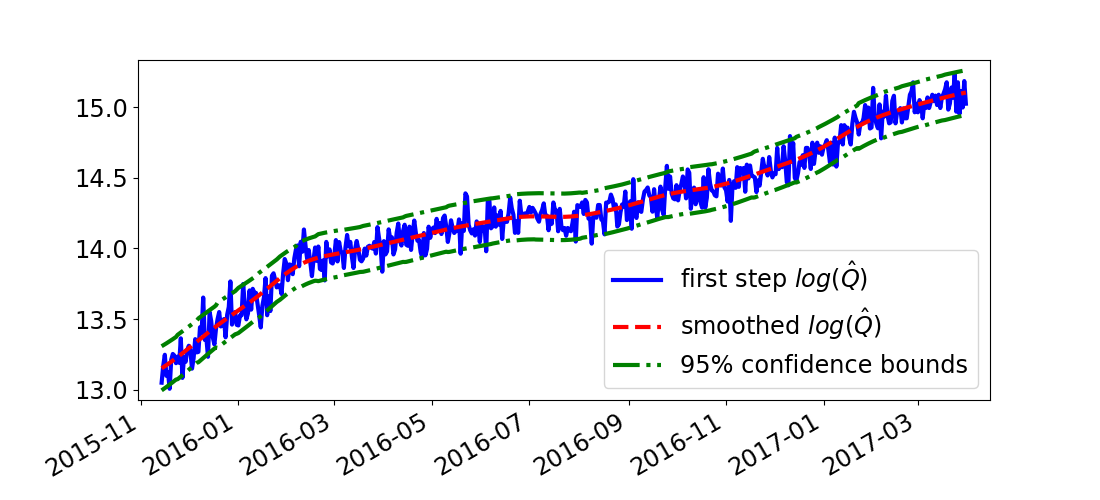
\includegraphics[scale=0.56]{images/comparaison_Q_Q_chap_log.png}
\end{figure}


%
%\section{The 2017 Bubble and its Aftermath}
%
%\label{app:Bubble}
%
%\begin{figure}[]
%\caption{The 2017 Bubble}
%\label{fig:failure_today}\centering
%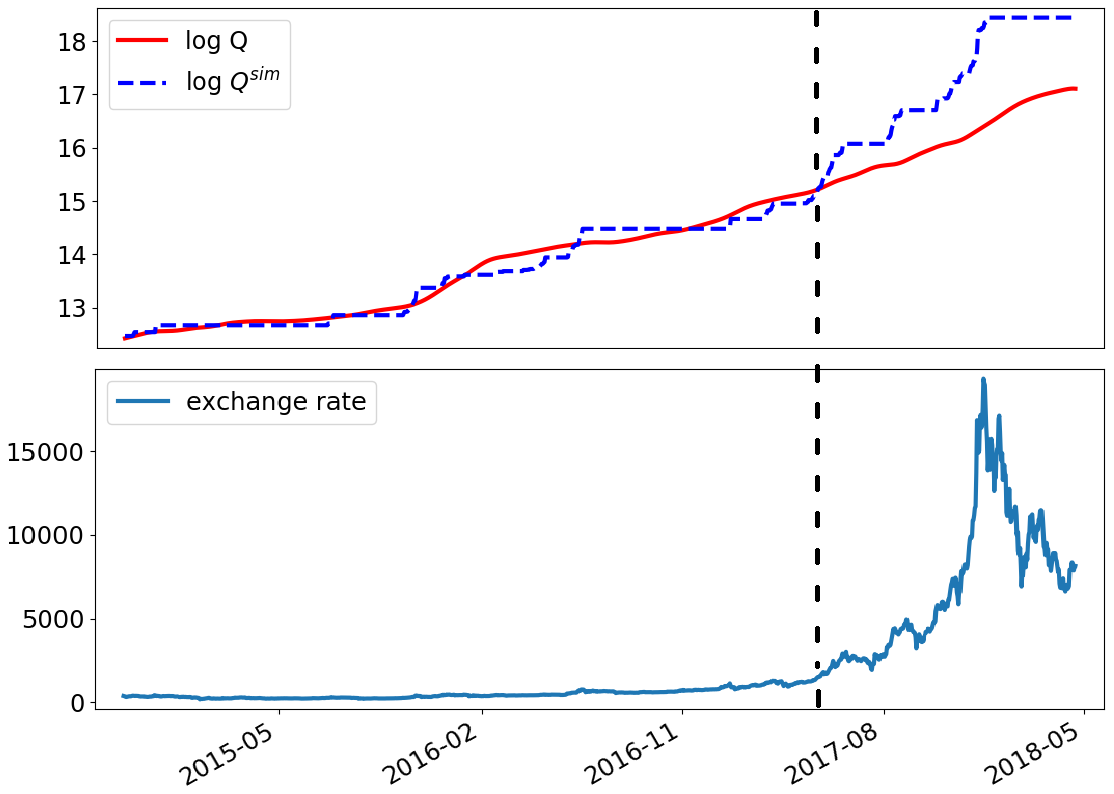
\includegraphics[scale=0.45]{images/failure_today5}
%\end{figure}
%
%\begin{figure}[]
%\caption{After the Bubble}
%\label{fig:after_bubble}\centering
%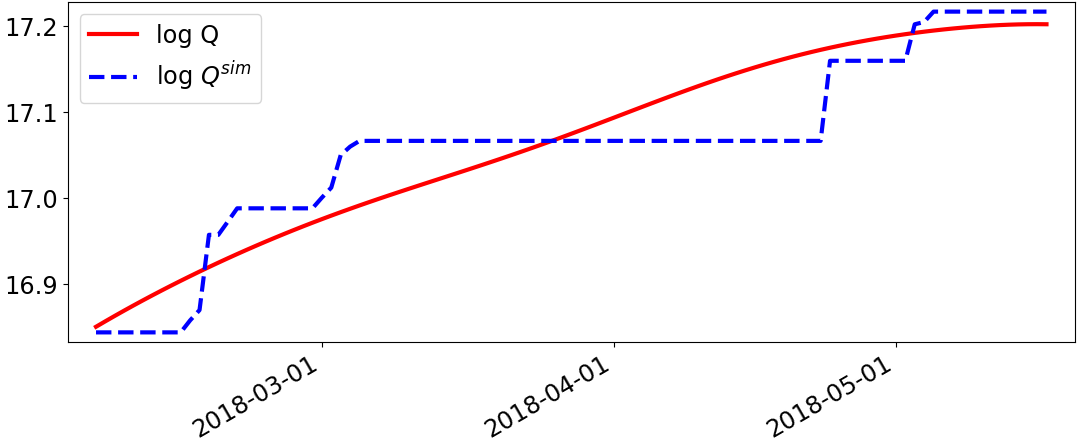
\includegraphics[scale=0.45]{images/apres_bulle}
%\caption*{Note: The simulated hashrate is reinitialized at the beginning of this simulation's period (2018/02/05).}
%\end{figure}

\section{Block bootstrap}
\label{app:block_bootstrap}

Since our data are time series, we resort to block bootstrap to estimate the standard deviations of our estimates. We follow the following procedure. Then, we compute the returns $dR$ and $dQ$ of the series $R$ and $Q$. Second, we divide those series of returns into blocks. A bootstrap random draw consists in the drawing with replacement of a series of blocks, which has the same length as the series observed in the data. For instance, if we divide our data in five blocks [1|2|3|4|5], then [2|4|2|3|4] or [5|5|2|1|5] could be bootstrap series. For a bootstrap draw $b$, we then obtain two series $dR_b$ and $dQ_b$. Starting with fixed initial values for $R$ and $Q$, we create series $R_b$ and $Q_b$ from the series of returns. Note that applying the bootstrap procedure on $R$ and $Q$ directly instead of the series of returns would not make any sense since the two series are not stationary. We finally estimate the parameters using our minimization procedure, with $R_b$ and $Q_b$ as input, and repeat the drawing and estimation 100 times in order to estimate the parameters' standard deviations.
It is important to note that for a given change in the exchange rate, miners' behavior crucially depends on how far $P$ is from the barrier. As a result, for our procedure to make sense (that is to say, to create bootstrap series which could have happened in the real life), the ratio of $P$ and the barrier must have the same value at the beginning of each block. We pick our blocks under this constraint.


\section{Out-of-sample experiments}

\label{app:out_of_sample}

We assess the model's ability to match
out-of-sample data by dividing the second period into a fit period and a
test period. We calibrate $a$ and $\overline{P}_0$ on the fit period only
and find that, even when the fit period is short, the calibrated
values remain close to the ones based on the full sample. Hence,  as illustrated in Figure \ref{fig:out-of-sample},
the predicted hashrate stays accurate several years after the end of the fit period.


\begin{figure}[H]
\caption{Out-of-Sample Experiment}
\label{fig:out-of-sample}\centering
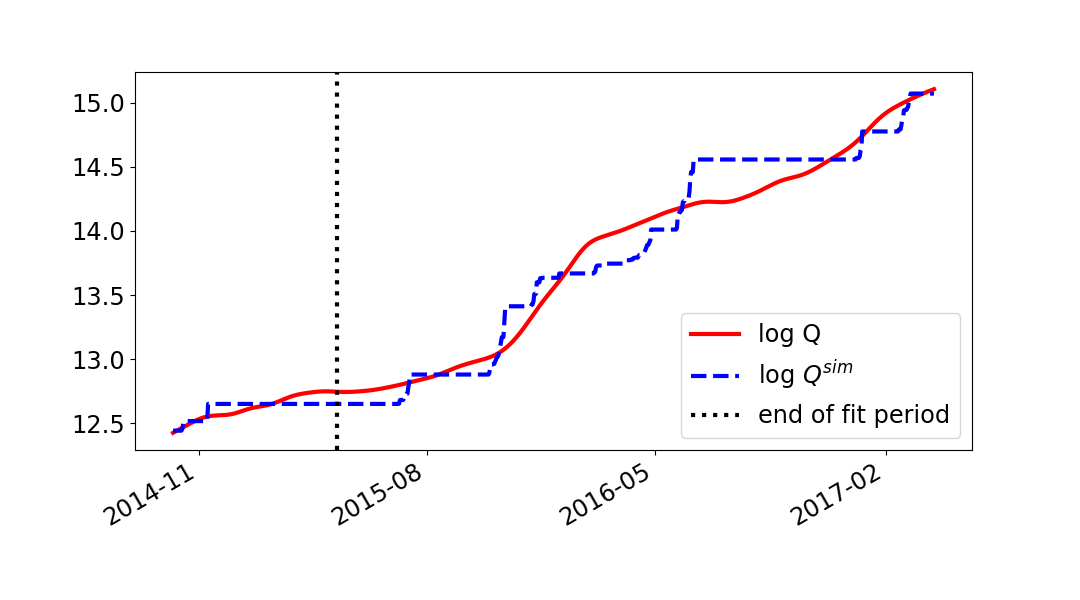
\includegraphics[scale=0.5]{images/out_of_sample_test.png}
\caption*{Note: The fit period is the shortest one for which the overall fit remains
accurate.}
\end{figure}

Note, however, that out-of-sample tests are much less conclusive for the
first period because the hashrate increases only at the beginning and at
the end of that period. Hence, if we split the first data sample into a fit
and a test period, the payoffs do not hit the reflecting barrier often
enough to deliver a reliable calibration.



\section{Fully reversible investments}
\label{app:totally reversible investments}

During the first subperiod, miners do not use specific mining hardware. Hence, the assumption that their investment is irreversible is less obvious than for our second period. To assess its accuracy, we estimate here a model with fully reversible investment. Figure \ref{fig:reversible_model_1} shows that the hashrate predicted by the reversible model fail to fits the data.

\bigskip

\begin{figure}[H]
\caption{Model with Totally Irreversible Investment}
\label{fig:reversible_model_1}
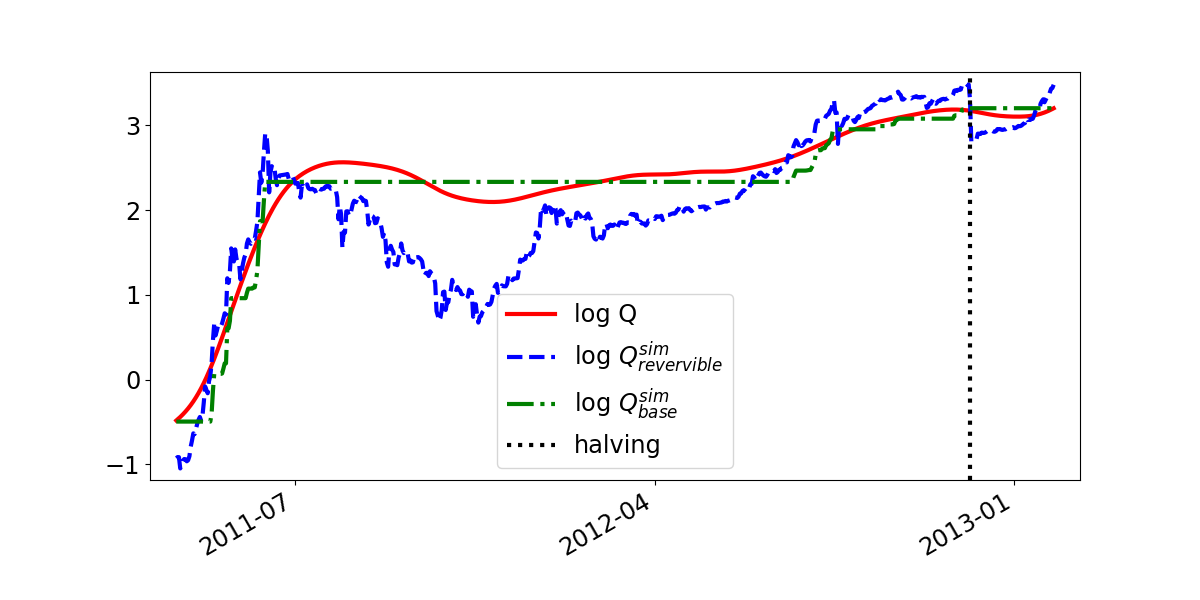
\includegraphics[scale=0.55]{images/Q_reversible_1}
\caption*{Note: Reversible model simulated under the free entry assumption. Since miners break even, payoffs are always set equal to the operational costs.}
\end{figure}



\section{Derivation of payoffs density $f^e$}
\label{app:Density_f}

\noindent \textbf{Lemma 1.} \emph{Let Assumptions \ref{hyp:continuous_update}, \ref%
{hyp:GBM}, \ref{hyp:rate_TP} and \ref{hyp:miners_myopic2} hold true. Then, for
all $t>0$, the density of $P_t$ conditional on the barrier being reached at
time $\tau<t$ reads
\begin{align*}
f_{P_t|P_\tau=\overline{P}_\tau}^e(x)&=\left(\frac{1}{x}\right)\left\{\left(%
\frac{1}{\sigma \sqrt{t}}\right)\phi\left(\frac{\log(\overline{P}%
_\tau)-\log(x)+\left(\alpha-\frac{\sigma^2}{2}\right)t}{\sigma \sqrt{t}}%
\right)\right. \\
&~~~~+\exp\left[\left(\log(\overline{P}_\tau)-\log(x)-at\right)\left(1-2%
\left(\frac{a+\alpha}{\sigma^2}\right)\right)\right] \\
&~~~~ \times \left[\left(2\left(\frac{a+\alpha}{\sigma^2}\right)-1\right)%
\Phi\left(\frac{\log(x)-\log(\overline{P}_\tau)+\left(2a+\alpha-\frac{%
\sigma^2}{2}\right)t}{\sigma \sqrt{t}}\right)\right. \\
&~~~~\left.\left.+\left(\frac{1}{\sigma \sqrt{t}}\right)\phi\left(\frac{%
\log(x)-\log(\overline{P}_\tau)+\left(2a+\alpha-\frac{\sigma^2}{2}\right)t}{%
\sigma \sqrt{t}}\right)\right]\right\}\mathds{1}_{]0,\overline{P}_t]}(x),
\end{align*}
where $\phi$ and $\Phi$ are the density and the cumulative distribution
function of the standard normal distribution, respectively.}

\bigskip

\begin{proof}
Since Assumption \ref{hyp:miners_myopic2} implies Assumption \ref%
{hyp:miners_myopic}, Proposition \ref{prop:industry-eq-variable-costs}
applies and we know that there exists a $\overline{P}_0$ such that $(P_t,%
\overline{P}_t=\overline{P}_0/A_t)$ is an industry equilibrium. Moreover,
Assumption \ref{hyp:miners_myopic2} also implies that the anticipated $P_t$
follows a GBM when $P_t<\overline{P}_t$ because the hashrate $Q_t$ remains
constant. Hence the anticipated $P_t$ follows a GBM reflected at $\overline{P%
}_0/A_t$. The density of a positive Brownian motion reflected at 0 and which
starts at 0 is given in \citeauthor{Harrison} (\citeyear{Harrison}). We now
show that it can be applied to the logarithm of $P$.

Without loss of generality, we can set the hitting time $\tau = 0$. Then $%
R_0/Q_0=\overline{P}_0$ because we are looking for a density conditional on $%
P_0=\overline{P}_0$. Hence the hashrate $Q_t$ is given by $
Q_t=\mathop{\sup}\limits_{0\leq s\leq t}A_sR_s/\overline{P}_0$.
Replacing this expression into the decomposition of $A_tP_t$, we find that
\begin{align*}
\log(A_tP_t)&=\log(A_tR_t)-\log(Q_t) \\
&=\log(A_tR_t)-\mathop{\sup}\limits_{0\leq s\leq t}\log(A_s R_s)+\log(%
\overline{P}_0) \\
&=\log(\overline{P}_0)-\left[-\log(A_t R_t)-\mathop{\inf}\limits_{0\leq
s\leq t}(-\log(A_s R_s))\right] \\
&= \log(\overline{P}_0)-Z_t,
\end{align*}
where $Z_t$ follows a positive Brownian motion with parameters $%
\left(\sigma^2/2-a-\alpha,\sigma\right)$, reflected at $0$ and with initial
condition $Z_0=0$. We know from \citeauthor{Harrison} (\citeyear{Harrison})
that, for all $x\geq0$, $\Pr\left(Z_t\leq x\right)=\Phi\left(\frac{x-\left(%
\frac{\sigma^2}{2}-a-\alpha\right) t}{\sigma \sqrt{t}}\right)-e^{\frac{%
2\left(\frac{\sigma^2}{2}-a-\alpha\right) x}{\sigma^2}}\Phi\left(\frac{%
-x-\left(\frac{\sigma^2}{2}-a-\alpha\right) t}{\sigma \sqrt{t}}\right)$.
Straightforward differentiation of this expression yields the solution for $%
f^e$.

\end{proof}

\section{Price of mining hardware}

\label{app:Price_data_2018}

\bigskip
\bigskip

\scalebox{1.05}{
\begin{tabular}{lcccc}
Name of rig & available on & hashpower (Th/s) & power (Watts) & price (\$) \\ \hline\hline
\multirow{2}*{Bitmain S1} & 2013/12/01 & 0.18 & 360 & 300\\
& \multicolumn{4}{c}{\url{https://en.bitcoin.it/wiki/Mining_hardware_comparison}} \\ \hline
\multirow{2}*{Bitmain S2} & 2014/04/01 & 1 & 1100 & 2260\\
& \multicolumn{4}{c}{\url{https://en.bitcoin.it/wiki/Mining_hardware_comparison}}\\ \hline
\multirow{2}*{Bitmain S3} & 2014/07/01 & 0.441 & 340 & 382\\
& \multicolumn{4}{c}{\url{https://en.bitcoin.it/wiki/Mining_hardware_comparison}} \\ \hline
\multirow{2}*{Bitmain S4} & 2014/10/01 & 2 & 1400 & 1400\\
& \multicolumn{4}{c}{\url{https://en.bitcoin.it/wiki/Mining_hardware_comparison}} \\ \hline
\multirow{2}*{Bitmain S5} & 2015/01/01 & 1.15 & 590 & 370\\
& \multicolumn{4}{c}{\url{https://en.bitcoin.it/wiki/Mining_hardware_comparison}} \\ \hline
\multirow{2}*{Bitmain S7} & 2015/09/01 & 4.86 & 1210 & 1823\\ \
& \multicolumn{4}{c}{\url{https://en.bitcoin.it/wiki/Mining_hardware_comparison}} \\ \hline
\multirow{2}*{Bitmain S9} & 2016/08/01 & 14 & 1375 & 2400\\
& \multicolumn{4}{c}{\url{https://en.bitcoin.it/wiki/Mining_hardware_comparison}} \\ \hline
\multirow{2}*{Bitmain S9} & 2018/01/01 & 14 & 1375 & 5179\\
& \multicolumn{4}{c}{\scriptsize{\url{https://camelcamelcamel.com/Antminer-S9-~13TH-Bitcoin-12-1600/product/B01LX6EVNI}}}\\ \hline
\multirow{2}*{Pangolin M10} & 2018/07/24 & 33 & 2150 & 2000\\
& \multicolumn{4}{c}{\url{https://bitcointalk.org/index.php?topic=4737927.0}} \\ \hline
\multirow{2}*{Pangolin M20} & 2019/05/20 & 48 & 2300 & 1450\\
& \multicolumn{4}{c}{\url{https://bitcointalk.org/index.php?topic=5120959.0}}
\end{tabular}
}

\begin{figure}[H]
\caption{Price Data for Mining Rigs}
\label{fig:price_2018}\centering
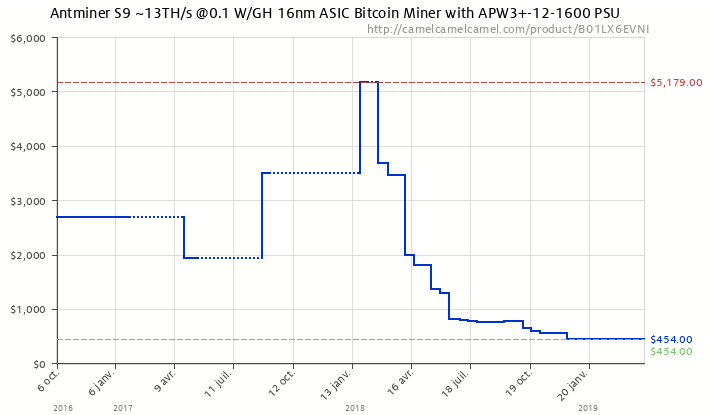
\includegraphics[scale=0.8]{images/S9_price_history}
\end{figure}




%
%\section{Mining Pools}
%\textbf{COMMENT JULIEN:
%\begin{itemize}
%  \item RELATE TO HE ET AL. PAPER.
%  \item DISCUSS WHAT HAPPENS TO ESTIMATES IF WE ARBITRARILY SHIFT COSTS AROUND ARRIVAL DATE OF MINING POOLS.
%\end{itemize}}


\section{Model with time-to-build}

\label{app:T2B}


The characterization of the equilibrium with time-to-build is borrowed from
\citeauthor{Grenadier2000} (\citeyear{Grenadier2000}). We outline the logic of the proof and refer readers to the
paper for more details.\ The first step of the proof consists in showing
that the equilibrium can be derived solving the problem of a single agent
that maximizes a "fictious" objective function. As in \citeauthor{Lucas} (\citeyear{Lucas}), the decentralized equilibrium maximizes social
welfare. Hence it can also be derived as an optima from the social
planner's perspective.

\paragraph{Equivalence between central planner and decentralized solutions.}

Our first task is to define the objective function.\ The flow benefits are
equal to the area under the payoff functions of miners so that $B\left(
R,Q\right) =\int_{0}^{Q}P\left( R,x\right) dx=\int_{0}^{Q}\left( R/x\right)
dx=R\log (Q)$. Since the central planner seeks to maximize benefits net of
costs, he solves the following problem%
\begin{eqnarray*}
J\left( R_{t},Q_{t},t\right)  &=&\max_{\left\{ Q_{s}\right\} _{s>t}}\mathbb{E%
}_{t}\left[ \int_{t}^{\infty }e^{-r(s-t)}\left( \left[ B\left(
R_{s},Q_{s}\right) -\int_{0}^{s}C_{\tau }dQ_{\tau }\right]
ds-I_{s}dQ_{s}\right) \right]  \\
&=&\max_{\left\{ Q_{s}\right\} _{s>t}}\mathbb{E}_{t}\left[ \int_{t}^{\infty
}e^{-r(s-t)}\left( \left[ B\left( R_{s},Q_{s}\right)
-C_{0}\int_{0}^{s}e^{-a\tau }dQ_{\tau }\right] ds-e^{-as}I_{0}dQ_{s}\right) %
\right]  \\
&=&\max_{\left\{ Q_{s}\right\} _{s>t}}\mathbb{E}_{t}\left[ \int_{t}^{\infty
}e^{-r(s-t)}\left( R_{s}\log (Q_{s})ds-e^{-as}\left( I_{0}+\frac{C_{0}}{r}%
\right) dQ_{s}\right) \right] .
\end{eqnarray*}%
Defining $K_{t}\equiv e^{-at}\left( I_{0}+\frac{C_{0}}{r}\right) $ allows us
to rewrite the objective function as%
\begin{equation*}
J\left( R_{t},Q_{t},K_{t}\right) =\max_{\left\{ Q_{s}\right\} _{s>t}}\mathbb{E}_{t}
\left[ \int_{t}^{\infty }e^{-r(s-t)}\left( R_{s}\log
(Q_{s})ds-K_{s}dQ_{s}\right) \right]
\end{equation*}%
Hence the value function of the planner satisfies the following differential
equation%
{ \scriptsize
\begin{equation}
rJ\left( R_{t},Q_{t},K_{t}\right) =R_{t}\log (Q_{t})+\alpha R_{t}J_{R}\left(
R_{t},Q_{t},K_{t}\right) +\frac{\sigma ^{2}R_{t}^{2}}{2}J_{RR}\left(
R_{t},Q_{t},K_{t}\right) -aK_{t}J_{K}\left( R_{t},Q_{t},K_{t}\right) ,
\label{HJB_planner}
\end{equation}
}%
subject to the value matching and smooth-pasting conditions%
\begin{eqnarray*}
\frac{\partial J\left( \overline{R}(Q,K),Q,K\right) }{\partial Q} &=&K, \\
\frac{\partial J\left( \overline{R}(Q,K),Q,K\right) }{\partial Q\partial R}
&=&0.
\end{eqnarray*}%
Since $\left( \ref{HJB_planner}\right) $ holds identically along the
optimal path, we can differentiate it with respect to $Q$ to obtain%
\begin{equation*}
rj\left( R_{t},Q_{t},K_{t}\right) =\frac{R_{t}}{Q_{t}}+\alpha
R_{t}j_{R}\left( R_{t},Q_{t},K_{t}\right) +\frac{\sigma ^{2}R_{t}^{2}}{2}%
j_{RR}\left( R_{t},Q_{t},K_{t}\right) -aK_{t}j_{K}\left(
R_{t},Q_{t},K_{t}\right) ,
\end{equation*}%
where $j\left( R,Q,K\right) \equiv \partial J\left( R,Q,K\right) /\partial Q$
denotes the marginal value of mining capacity. The boundary conditions
above are therefore equivalent to%
\begin{eqnarray*}
j\left( \overline{R}(Q,K),Q,K\right)  &=&K, \\
\frac{\partial j\left( \overline{R}(Q,K),Q,K\right) }{\partial R} &=&0.
\end{eqnarray*}

The differential equation and boundary conditions are verified when (i) $%
\overline{R}(Q,K)=DQK$, for a constant $D$ that is yet to be determined; and
(ii) $j$ reads%
\begin{equation}
j\left( R_{t},Q_{t},K_{t}\right) =\frac{R_{t}/Q_{t}}{r-\alpha }-\left[ \frac{%
DK_{t}}{\beta (r-\alpha )}\right] \left( \frac{R_{t}/Q_{t}}{DK_{t}}\right)
^{\beta },  \label{eq:Solution_planner}
\end{equation}%
where $\beta $ is the positive root of the quadratic equation
\begin{equation*}
\mathcal{Q}(\beta )\equiv \frac{\sigma ^{2}}{2}\beta (\beta -1)+(\alpha
+a)\beta -a-r=0,
\end{equation*}%
and the constant $D=(r-\alpha )\beta /\left( \beta -1\right) .\ $Replacing $%
P_{t}=R_{t}/Q_{t}$,\ $K_{t}=K_{0}/A_{t}$ and $\overline{P}_{t}=DK_{t}$ into $%
\left( \ref{eq:Solution_planner}\right) $, we find that the optimal
investment strategy of the planner is identical to the entry rule of the
decentralized equilibrium.

\paragraph{Industry dynamics with time-to-build.}

Having shown that we can use a central planner to solve for the equilibrium,
we now introduce time-to-build. There is an exogenous delay $\delta $
between the time a new unit of hashpower is ordered and when it become
operational.\ Let $N_{t}$ denote the number of units that are currently in
the delivery pipeline because their purchase order occurred within $\left(
t-\delta ,t\right] $, and let $H_{t}=Q_{t}+N_{t}$ denote the "committed
hashpower" at date $t$.

The state of the economy is summarized by the following vector%
\begin{equation*}
\Omega _{t}=\left\{ R_{t},K_{t},Q_{t},N_{t},\Lambda _{t}\right\} ,\ \text{%
where\ }\Lambda _{t}\equiv \left\{ s\in \left( t-\delta ,t\right]
:Q_{t}>Q_{t^{-}}\right\} .
\end{equation*}%
The set $\Lambda _{t}\ $records all the dates at which hashpower has been
committed within the current delivery window $\left( t-\delta ,t\right] .$
Note that the investment cost $K_{t}$ has to be adjusted to take into
account the delivery delay so that $K_{t}=e^{-at }\left[I_{0}+e^{-r\delta }C_{0}/r\right].\ $%
Since $Q_{t}=H_{t-\delta }$, $B\left( R_{t},Q_{t}\right) =R_{t}\log
(H_{t-\delta })$ and the planner solves the following problem%
\begin{eqnarray}
&&J^{\delta }\left( R_{t},K_{t},Q_{t},N_{t},\Lambda _{t}\right)   \notag \\
&=&\mathbb{E}_{t}\left[ \left. \int_{t}^{t+\delta }e^{-r(s-t)}R_{s}\log
(H_{s-\delta })ds\right\vert R_{t},K_{t},Q_{t},N_{t},\Lambda _{t}\right]
\notag \\
&&+\max_{\left\{ H_{s}\right\} _{s>t}}\mathbb{E}_{t}\left[ \left.
\int_{t+\delta }^{\infty }e^{-r(s-t)}\left( R_{s}\log (H_{s-\delta
})ds-K_{s}dH_{s}\right) \right\vert R_{t},K_{t},Q_{t},N_{t},\Lambda _{t}%
\right]   \notag \\
&=&\mathbb{E}_{t}\left[ \left. \int_{t}^{t+\delta }e^{-r(s-t)}R_{s}\log
(H_{s-\delta })ds\right\vert R_{t},K_{t},Q_{t},N_{t},\Lambda _{t}\right]
\notag \\
&&+\max_{\left\{ H_{s}\right\} _{s>t}}\mathbb{E}_{t}\left[ \left.
\int_{t+\delta }^{\infty }e^{-r(s-t)}\left( R_{s}\log (H_{s-\delta
})ds-K_{s}dH_{s}\right) \right\vert R_{t},K_{t},H_{t},0,\emptyset \right]
\notag \\
&=&J^{\delta }\left( R_{t},K_{t},H_{t},0,\emptyset \right)   \notag \\
&&+\mathbb{E}_{t}\left[ \left. \int_{t}^{t+\delta }e^{-r(s-t)}R_{s}\log
(Q_{s-\delta })ds\right\vert R_{t},K_{t},Q_{t},N_{t},\Lambda _{t}\right]
\notag \\
&&-\mathbb{E}_{t}\left[ \left. \int_{t}^{t+\delta }e^{-r(s-t)}R_{s}\log
(Q_{s-\delta })ds\right\vert R_{t},K_{t},H_{t},0,\emptyset \right] .
\label{eq:J_T2B}
\end{eqnarray}
The second equality holds because the flow surplus at date $t+\delta $ only
depends on the amount of committed hashpower $H_{t}$. Hence the optimized
paths are identical under $\Omega _{t}=\left\{
R_{t},K_{t},Q_{t},N_{t},\Lambda _{t}\right\} $ and under the assumption that
all units currently in the pipeline are delivered, so that $\tilde{\Omega}%
_{t}=\left\{ R_{t},K_{t},Q_{t}+N_{t},0,\emptyset \right\} =\left\{
R_{t},K_{t},H_{t},0,\emptyset \right\} $.\ The last equality follows from
the definition of $J^{\delta }$. Note that the last two terms in $\left( \ref%
{eq:J_T2B}\right) $ are beyond the control of the planner at time $t.\ $%
Hence he seeks to maximize $J^{\delta }\left( R_{t},K_{t},H_{t},0,\emptyset
\right) \ $which we denote by $V^{\delta }\left( R_{t},H_{t},K_{t}\right) $.

Over the range in which $H_{t}$ remains constant, $V^{\delta }\left(
R_{t},H_{t},K_{t}\right) $ can be interpreted as the value of an industry
with $H_{t}$ completed units yielding a dividend flow of $R_{t}\log (H_{t})$%
.\ Hence the value function in the no-investment region satisfies the
differential equation%
\begin{equation*}
rV^{\delta }\left( R_{t},H_{t},K_{t}\right) =R_{t}\log (H_{t})+\alpha
R_{t}V_{R}^{\delta }\left( R_{t},H_{t},K_{t}\right) +\frac{\sigma
^{2}R_{t}^{2}}{2}V_{RR}^{\delta }\left( R_{t},H_{t},K_{t}\right)
-aK_{t}V_{K}^{\delta }\left( R_{t},H_{t},K_{t}\right) .
\end{equation*}%
Since the HJB equation is the same as that of the problem without delay $%
\left( \ref{HJB_planner}\right) $, its derivative with respect to installed
capacity, $v^{\delta }\left( R,H,K\right) \equiv \partial V^{\delta }\left(
R,H,K\right) /\partial H$, also admits a solution of the form%
\begin{equation}
v^{\delta }\left( R_{t},H_{t},K_{t}\right) =\frac{R_{t}/H_{t}}{r-\alpha }%
+D\left( H_{t},K_{t}\right) R_{t}^{\beta }.  \label{eq:V_T2B}
\end{equation}%
Let $\overline{R}^{\delta }(H,K)$ denote the level of $R_{t}$ at which
market entry is optimal.\ Then the value-matching condition reads%
\begin{eqnarray*}
V^{\delta }\left( \overline{R}^{\delta }(H,K),H,K\right)  &=&J^{\delta
}\left( \overline{R}^{\delta }(H,K),K,H,dH,\emptyset \right) -KdH \\
&=&V^{\delta }\left( \overline{R}^{\delta }(H,K),H+dH,K\right) -KdH \\
&&+\mathbb{E}\left[ \left. \int_{0}^{\delta }e^{-rt}R_{t}\log
(H)dt\right\vert R_{0}=\overline{R}^{\delta }(H,K)\right]  \\
&&-\mathbb{E}\left[ \left. \int_{0}^{\delta }e^{-rt}R_{t}\log
(H+dH)dt\right\vert R_{0}=\overline{R}^{\delta }(H,K)\right] .
\end{eqnarray*}%
Differentiating this condition yields%
\begin{equation}
v^{\delta }\left( \overline{R}^{\delta }(H,K),H,K\right) =\frac{\overline{R}%
^{\delta }(H,K)/H}{r-\alpha }\left[ 1-e^{-\left( r-\alpha \right) \delta }%
\right] +K.  \label{eq:VM_T2B}
\end{equation}%
The optimal value of\ $\overline{R}^{\delta }$ follows from the
smooth-pasting condition%
\begin{equation}
\frac{\partial v^{\delta }\left( \overline{R}^{\delta }(H,K),H,K\right) }{%
\partial R}=\frac{1-e^{-\left( r-\alpha \right) \delta }}{H\left( r-\alpha
\right) }.  \label{eq:SC_T2B}
\end{equation}
Combining $\left( \ref{eq:VM_T2B}\right) \ $and\ $\left( \ref{eq:SC_T2B}%
\right) $ with the general solution $\left( \ref{eq:V_T2B}\right) $, yields
the following solution%
\begin{equation*}
v^{\delta }\left( R_{t},H_{t},K_{t}\right) =\frac{R_{t}/H_{t}}{r-\alpha }-%
\left[ \frac{DK_{t}e^{-\left( r-\alpha \right) \delta }}{\beta (r-\alpha )}%
\right] \left( \frac{R_{t}/H_{t}}{DK_{t}}\right) ^{\beta },
\end{equation*}%
where $\beta $ is the positive root of the quadratic equation
\begin{equation*}
\mathcal{Q}(\beta )\equiv \frac{\sigma ^{2}}{2}\beta (\beta -1)+(\alpha
+a)\beta -a-r=0,
\end{equation*}%
and the constant $D$ reads
\begin{equation*}
D=\frac{\beta (r-\alpha )}{\left( \beta -1\right) e^{-\left( r-\alpha
\right) \delta }}.
\end{equation*}%
Finally, dividing the block rewards $R$ by $H$ yields the expression
of the reflecting barrier, which is indeed decreasing at the rate of
technological progress since
\begin{equation*}
\overline{P}_{t}^{\delta }=\frac{\overline{R}^{\delta }(H_{t},K_{t})}{H_{t}}=%
\frac{\beta (r-\alpha )}{\left( \beta -1\right) e^{-\left( r-\alpha \right)
\delta }}K_{t}=e^{-at}\overline{P}_{0}^{\delta }.
\end{equation*}


\section{Model with convex adjustment costs}
\label{app:Section_convex}

Let $q_{t}$ denote investment in hashpower so that $Q_{t}=Q_{0}+\int_{0}^{t} q_{s}ds$. Using $%
c\left( q,Q,K\right) $ to denote the overall entry costs as a function of $q$%
, the planner's value function must satisfy the following HJB equation
\begin{eqnarray}
rJ\left( R_{t},Q_{t},K_{t}\right)  &=&\max_{q_{t}}\left\{ R_{t}\log
(Q_{t})-c\left( q_{t},Q_{t},K_{t}\right) +q_{t}J_{Q}\left(
R_{t},Q_{t},K_{t}\right) \right\}   \notag \\
&&+\alpha R_{t}J_{R}\left( R_{t},Q_{t},K_{t}\right) +\frac{\sigma
^{2}R_{t}^{2}}{2}J_{RR}\left( R_{t},Q_{t},K_{t}\right) -aK_{t}J_{K}\left(
R_{t},Q_{t},K_{t}\right).~~~~
\label{eq:HJB_nonlinear}
\end{eqnarray}%
We assume that%
\begin{equation*}
c\left( q,Q,K\right) =\left\{
\begin{array}{l}
Kq\left[ 1+\left( \frac{q}{Q}\right) ^{\eta }\right] \text{,}\ \text{with }%
\eta >1\text{,}\ \text{for }q\geq 0\text{,} \\
g\left( q\right) >0\text{,}\ \text{with }g^{\prime }\left( q\right) >0\text{,%
}\ \text{for }q<0.%
\end{array}%
\right.
\end{equation*}%
As in \citeauthor{Abel} (\citeyear{Abel}), assuming that reducing $Q$ has a
positive cost effectively ensures that investment is irreversible. Hence we
have%
\begin{equation}
q_{t}=\max \left\{ 0,\left( \frac{j\left( R_{t},Q_{t},K_{t}\right) /K_{t}-1}{%
1+\eta }\right) ^{\frac{1}{\eta }}Q_{t}\right\} ,
\label{eq:Opt_invt_nonlinear}
\end{equation}%
where $j\left( R_{t},Q_{t},K_{t}\right) \equiv J_{Q}\left(
R_{t},Q_{t},K_{t}\right) .$

The HJB equation $\left( \ref{eq:HJB_nonlinear}\right)$ can be differentiated
with respect to $Q$ since it holds identically. Hence the shadow value of
of $Q$ satisfies the following HJB
\begin{eqnarray}
rj\left( R_{t},Q_{t},K_{t}\right)  &=&\frac{R_{t}}{Q_{t}}-c_{Q}\left(
q_{t},Q_{t},K_{t}\right) +q\left( j\left( R_{t},Q_{t},K_{t}\right)
,Q_{t},K_{t}\right) j_{Q}\left( R_{t},Q_{t},K_{t}\right)   \notag \\
&&+\alpha R_{t}j_{R}\left( R_{t},Q_{t},K_{t}\right) +\frac{\sigma
^{2}R_{t}^{2}}{2}j_{RR}\left( R_{t},Q_{t},K_{t}\right) -aK_{t}j_{K}\left(
R_{t},Q_{t},K_{t}\right)   \notag \\
&&+\underset{=0\ if\ q_{t}>0}{\underbrace{\left[ j\left(
R_{t},Q_{t},K_{t}\right) -c_{q}\left( q_{t},Q_{t},K_{t}\right) \right] }}%
\underset{=0\ if\ q_{t}=0}{\underbrace{q_{j}\left( j\left(
R_{t},Q_{t},K_{t}\right) ,Q_{t},K_{t}\right) }}j_{Q}\left(
R_{t},Q_{t},K_{t}\right) .~~~~  \label{eq:HJB_tobinq_non_linear}
\end{eqnarray}%

In order to reduce the state space, we guess that $j\left( R,Q,K\right)
=Kj\left( \frac{R}{QK},1,1\right)$. We now verify that this conjecture is indeed correct by proving
that it satisfies the HJB equation. Readers interested in a more systematic analysis
can read Lemma 2 below, where we prove that $j$ is homogenous of degree zero in $\left(
R,Q\right)$, and homogenous of degree one in $\left(
R,K\right)$. Since $j\left( R,Q,K\right)
=Kj\left( \frac{R}{QK},1,1\right)$, it must hold true that
\begin{eqnarray*}
j_{R}\left( R,Q,K\right)  &=&\frac{1}{Q}j_{1}\left( \frac{R}{QK},1,1\right) ,
\\
j_{RR}\left( R,Q,K\right)  &=&\frac{1}{Q^{2}K}j_{1}\left( \frac{R}{QK}%
,1,1\right) , \\
j_{Q}\left( R,Q,K\right)  &=&-\frac{R}{Q^{2}}j_{1}\left( \frac{R}{QK}%
,1,1\right) , \\
j_{K}\left( R,Q,K\right)  &=&j\left( \frac{R}{QK},1,1\right) -\frac{R}{QK}%
j_{1}\left( \frac{R}{QK},1,1\right) .
\end{eqnarray*}%
Replacing the four conditions above into the HJB equation\ $\left( \ref%
{eq:HJB_tobinq_non_linear}\right) \ $yields%
{ \scriptsize
\begin{eqnarray}
rj\left( R_{t},Q_{t},K_{t}\right)  &=&\frac{R_{t}}{Q_{t}}+K_{t}\eta \left(
\frac{q\left( R_{t},Q_{t},K_{t}\right) }{Q_{t}}\right) ^{1+\eta }+\alpha
\frac{R_{t}}{Q_{t}}j_{1}\left( \frac{R_{t}}{Q_{t}K_{t}},1,1\right) +\frac{%
\sigma ^{2}R_{t}^{2}}{2Q_{t}^{2}K_{t}}j_{11}\left( \frac{R_{t}}{Q_{t}K_{t}}%
,1,1\right)   \notag \\
&&-aK_{t}\left[ j\left( \frac{R_{t}}{Q_{t}K_{t}},1,1\right) -\frac{R_{t}}{%
Q_{t}K_{t}}j_{1}\left( \frac{R_{t}}{Q_{t}K_{t}},1,1\right) \right] -q\left(
\frac{R_{t}}{Q_{t}K_{t}},1,1\right) Q_{t}\left[ \frac{R_{t}}{Q_{t}^{2}}%
j_{1}\left( \frac{R_{t}}{Q_{t}K_{t}},1,1\right) \right],~~~~\label{HJB_reduced_intermediate2}
\end{eqnarray}%
}
where we have used the fact that%
\begin{eqnarray*}
q\left( R_{t},Q_{t},K_{t}\right)  &=&\left( \frac{j\left(
R_{t},Q_{t},K_{t}\right) /K_{t}-1}{1+\eta }\right) ^{\frac{1}{\eta }}Q_{t} \\
&=&\left( \frac{j\left( \frac{R_{t}}{Q_{t}K_{t}},1,1\right) -1}{1+\eta }%
\right) ^{\frac{1}{\eta }}Q_{t} \\
&=&q\left( \frac{R_{t}}{Q_{t}K_{t}},1,1\right) Q_{t}.
\end{eqnarray*}
Replacing $%
j\left( R_{t},Q_{t},K_{t}\right) \ $with$\ K_{t}j\left( \frac{R_{t}}{%
Q_{t}K_{t}},1,1\right) $ on the left-hand side of $\left( \ref{HJB_reduced_intermediate2}\right) $,
and dividing by $K_{t}$, yields an equation that depends on $R_{t}/\left( Q_{t}K_{t}\right) $ only
{ \footnotesize
\begin{eqnarray*}
rj\left( \frac{R_{t}}{Q_{t}K_{t}},1,1\right)  &=&\frac{R_{t}}{Q_{t}K_{t}}%
+\eta q\left( \frac{R_{t}}{Q_{t}K_{t}},1,1\right) ^{1+\eta }+\alpha \frac{%
R_{t}}{Q_{t}K_{t}}j_{1}\left( \frac{R_{t}}{Q_{t}K_{t}},1,1\right) +\frac{%
\sigma ^{2}}{2}\left( \frac{R_{t}}{Q_{t}K_{t}}\right) ^{2}j_{11}\left( \frac{%
R_{t}}{Q_{t}K_{t}},1,1\right)  \\
&&-a\left[ j\left( \frac{R_{t}}{Q_{t}K_{t}},1,1\right) -\frac{R_{t}}{%
Q_{t}K_{t}}j_{1}\left( \frac{R_{t}}{Q_{t}K_{t}},1,1\right) \right] -\frac{%
R_{t}}{Q_{t}K_{t}}q\left( \frac{R_{t}}{Q_{t}K_{t}},1,1\right) j_{1}\left(
\frac{R_{t}}{Q_{t}K_{t}},1,1\right) .
\end{eqnarray*}
}

We have derived an ODE that only depends on $R_{t}/\left( Q_{t}K_{t}\right) $
and which solves the original PDE\ while satisfying the optimality condition
for investment. Replacing $q\ $with its expression in $\left( \ref%
{eq:Opt_invt_nonlinear}\right) $ and using\ $x_{t}$ to denote$\ R_{t}/\left(
Q_{t}K_{t}\right) $, we finally obtain the simplified HJB\ equation%
\begin{equation*}
\resizebox{\textwidth}{!}
{$
\left( r+a\right) \tilde{j}\left( x_{t}\right) =\left\{
\begin{array}{l}
x_{t}+\eta \left( \frac{\tilde{j}\left( x_{t}\right) -1}{1+\eta }\right) ^{%
\frac{1+\eta }{\eta }}+\left( \alpha +a-\left[ \frac{\tilde{j}\left(
x_{t}\right) -1}{1+\eta }\right] ^{\frac{1}{\eta }}\right) x_{t}\tilde{j}%
^{\prime }\left( x_{t}\right) +\frac{\sigma ^{2}}{2}x_{t}^{2}\tilde{j}%
^{\prime \prime }\left( x_{t}\right) ,\ \text{when }\tilde{j}\left(
x_{t}\right) \geq 1, \\
x_{t}+\left( \alpha +a\right) x_{t}\tilde{j}^{\prime }\left( x_{t}\right) +%
\frac{\sigma ^{2}}{2}x_{t}^{2}\tilde{j}^{\prime \prime }\left( x_{t}\right)
,\ \text{when }\tilde{j}\left( x_{t}\right) <1.%
\end{array}%
\right.
$}
\end{equation*}


For our
calibration, we generalize the cost function to take into account the
distinction between the investment and the operating costs. More precisely, we assume
that, as in the body of the paper, the marginal costs of entry are given by
\begin{equation*}
I\left( q,Q,A\right) =\frac{I_{0}}{A}\left[ 1+\left( \frac{q}{bQ}\right)
^{\eta }\right] \text{,}\ \text{for }q\geq 0\text{.}
\end{equation*}%
Then the overall entry costs read%
\begin{eqnarray*}
c\left( q_{t},Q_{t},K_{t}\right)  &=&\int_{0}^{q_{t}}I\left(
y,Q_{t},K_{t}\right) dy+q_{t}\frac{C_{t}}{r} \\
&=&K_{t}q_{t}\left[ 1+\left( \frac{q_{t}}{\tilde{b}Q_{t}}\right) ^{\eta }%
\right] ,
\end{eqnarray*}%
where $K_{t}=\left( I_{0}+C_{0}/r\right) /A_{t}=e^{-at}\left(
I_{0}+C_{0}/r\right) /A_{0}$,$\ $and $\tilde{b}\equiv b\left[ \frac{\left(
1+\eta \right) K_{0}}{I_{0}}\right] ^{1/\eta }$.\ Given that the optimal
entry flow solves%
\begin{equation*}
q\left( R_{t},Q_{t},K_{t}\right) =\max \left\{ 0,\left( \frac{j\left(
R_{t},Q_{t},K_{t}\right) /K_{t}-1}{1+\eta }\right) ^{\frac{1}{\eta }}\tilde{b%
}Q_{t}\right\} ,
\end{equation*}%
the HJB is now equivalent to
\begin{equation}
\resizebox{\textwidth}{!}
{$
\left( r+a\right) \tilde{j}\left( x_{t}\right) =\left\{
\begin{array}{l}
x_{t}+\eta \tilde{b} \left( \frac{\tilde{j}\left( x_{t}\right) -1}{1+\eta }\right) ^{%
\frac{1+\eta }{\eta }}+\left( \alpha +a-\left[ \frac{\tilde{j}\left(
x_{t}\right) -1}{1+\eta }\right] ^{\frac{1}{\eta }}\tilde{b}\right) x_{t}%
\tilde{j}^{\prime }\left( x_{t}\right) +\frac{\sigma ^{2}}{2}x_{t}^{2}\tilde{%
j}^{\prime \prime }\left( x_{t}\right) ,\ \text{when }\tilde{j}\left(
x_{t}\right) \geq 1, \\
x_{t}+\left( \alpha +a\right) x_{t}\tilde{j}^{\prime }\left( x_{t}\right) +%
\frac{\sigma ^{2}}{2}x_{t}^{2}\tilde{j}^{\prime \prime }\left( x_{t}\right)
,\ \text{when }\tilde{j}\left( x_{t}\right) <1.%
\end{array}%
\right.
$}
\label{eq:HJB_normalized}
\end{equation}



\begin{figure}[]
\caption{Convergence of Numerical Solution}
\label{fig:Iteration_HJB}\centering
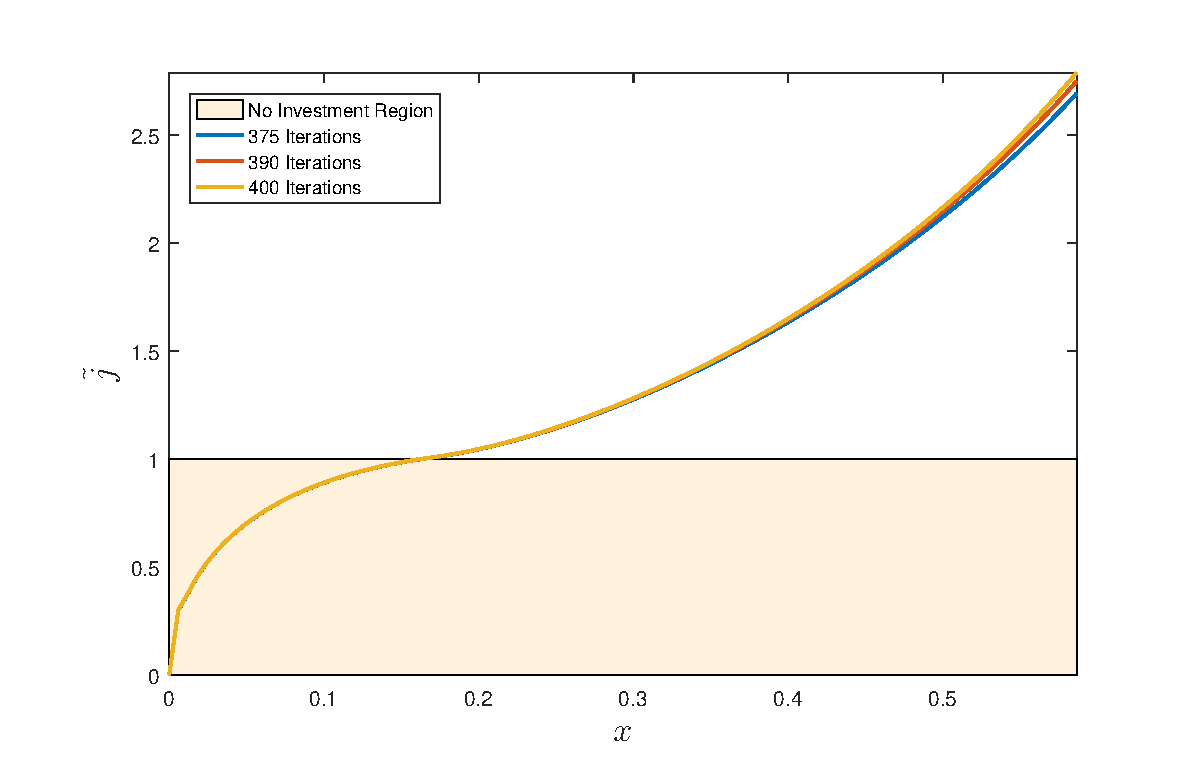
\includegraphics[scale=.6]{images/Iteration_HJB.eps}
\caption*{Note: Simulated solutions of the HJB equation (\ref{eq:HJB_normalized})
at different numbers of iterations.}
\end{figure}



\begin{figure}[]
\caption{Policy Function}
\label{fig:Policy}\centering
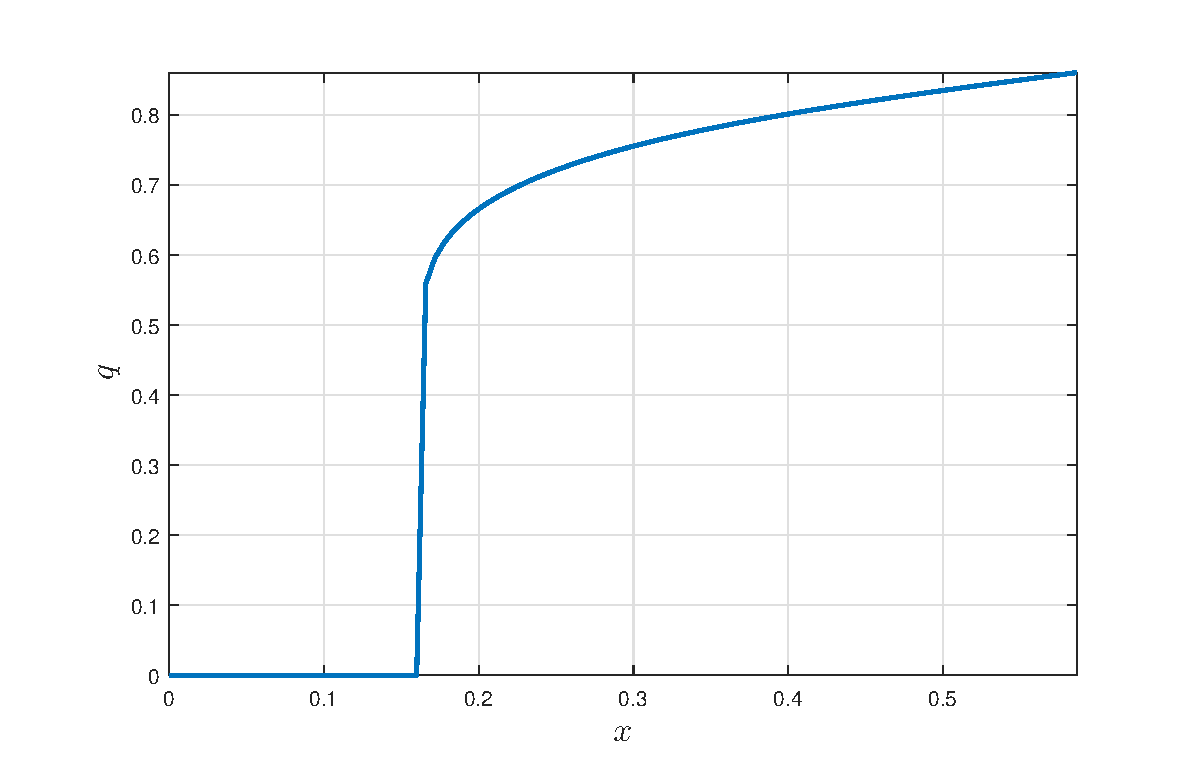
\includegraphics[scale=.6]{images/Policy.eps}
\caption*{Note: Calibrated policy function of the model with convex adjustment costs.}
\end{figure}


We use a finite-difference method to approximate the HJB equation, using
the value function with linear costs as our starting guess. We rely on the implicit Euler scheme in order to ensure that the
approximation is stable. The system of linearized equations is solved using
a generalization of the Gauss-Seidel iterative method known as the
successive-over-relaxation method. Solving for $j$ yields the investment rate
$q$ as a function of $P$, as well as the marginal costs of investment $c_q$.
As for the baseline model, we use the policy function to simulate the trajectory of the network hashrate
and also that of the investment costs.
The empirical moments are summarized by the vector $\mathbf{%
\hat{m}}$ which contains the actual hashrate of the network and the online price series described in
the Technical Appendix
\ref{app:Price_data_2018}. Using $\mathbf{m}(\mathbf{%
\upsilon )}$ to denote the simulated moments generated by the vector of
parameters $\upsilon \equiv \{a,\eta,b\}$, we compute the quadratic distances $d(\upsilon)\equiv
\left( \mathbf{m}(\mathbf{\upsilon})-\mathbf{\hat{m}}\right) \Omega \left(
\mathbf{m}(\mathbf{\upsilon} )-\mathbf{\hat{m}}\right)$, where $\Omega$ is a weighting
matrix that places equal weight on the hashrate and price data. Our calibrated vector
$\mathbf{\hat{\upsilon}}=\arg
\min_{\upsilon \in \mathbb{R}_{+}^{3}}d(\mathbf{%
\upsilon )}$.


Figure \ref{fig:Iteration_HJB} illustrates the convergence of our numerical procedure. It reports the simulated value function $\tilde{j}$
after different number of iterations. One can see that after 400 iterations, the incremental changes in the value function
are negligible, especially if one focuses on the region around the investment threshold $\tilde{j}(\overline{x})=1.$ The policy
function $q(x)$ of the calibrated model is reported in Figure \ref{fig:Policy}. Aggregate investment is nearly vertical
at the entry barrier $\overline{x}$, but is prevented from reaching an infinite intensity, as would be the case under linear costs,
by the convexity of the adjustment cost function.


We conclude our analysis of the model with convex costs with a Lemma that proves the validity of the normalization $j\left( R,Q,K\right)
=Kj\left( \frac{R}{QK},1,1\right)$.

\noindent \textbf{Lemma 1.}
%\label{Claim_homogeneity}
\emph{The shadow value of capital $j\left(
R_{t},Q_{t},K_{t}\right) $ is homogenous of degree zero in $\left(
R_{t},Q_{t}\right) $, and homogenous of degree one in $\left(
R_{t},K_{t}\right) $, i.e. $\ j\left( \lambda R_{t},\lambda
Q_{t},K_{t}\right) =j\left( R_{t},Q_{t},K_{t}\right) $ and $\ j\left(
\lambda R_{t},Q_{t},\lambda K_{t}\right) =\lambda j\left(
R_{t},Q_{t},K_{t}\right) $ for all $\lambda >0.$
}
%\end{lem}

\begin{proof}
Let $q_{\cdot }^{\ast }\left( R_{t},Q_{t},K_{t}\right) =\left\{ q_{s}^{\ast
}\left( R_{s},Q_{s},K_{s}\right) \right\} _{s\geq t}\ $denote the optimal
investment path starting at $\left( R_{t},Q_{t},K_{t}\right) .\ $Consider a
planner which faces the initial condition $\left( \lambda R_{t},\lambda
Q_{t},K_{t}\right) $ where $\lambda >0,\ $and implements the investment
strategy $q_{\cdot }^{\lambda }=\lambda q_{\cdot }^{\ast }\left(
R_{t},Q_{t},K_{t}\right) $. Then the hashpower resulting from $q_{\cdot
}^{\lambda }$ satisfies
\begin{equation*}
Q_{s}^{\lambda }=\lambda Q_{t}+\int_{s}^{t}q_{\tau}^{\lambda }d\tau=\lambda \left[
Q_{t}+\int_{s}^{t}q_{\tau}^{\ast }d\tau\right] =\lambda Q_{s}^{\ast },\ \text{for all }s\geq t.
\end{equation*}%
Moreover, since $R_{t}$ follows a geometric Brownian motion%
\begin{equation*}
\Pr \left\{ \left. R_{s}\leq x\right\vert R_{t}\right\} =\Pr \left\{ \left.
\lambda R_{s}\leq \lambda x\right\vert \lambda R_{t}\right\} ,\ \text{for
all }s>t\ \text{and all }x\in \mathbb{R}_{+},
\end{equation*}%
we have%
\begin{eqnarray*}
V^{\lambda }\left( \lambda R_{t},\lambda Q_{t},K_{t}\right)  &=&\mathbb{E}%
_{t}\left[ \int_{t}^{\infty }e^{-r\left( s-t\right) }\left( \frac{\lambda
R_{s}}{\lambda Q_{s}^{\ast }}-\frac{\partial c\left( q_{s}^{\lambda
},Q_{s}^{\lambda },K_{s}\right) }{\partial Q_{s}}\right) ds\right]  \\
&=&\mathbb{E}_{t}\left[ \int_{t}^{\infty }e^{-r\left( s-t\right) }\left(
\frac{R_{s}}{Q_{s}^{\ast }}-\eta K_{t}\left( \frac{q_{s}^{\ast }}{%
Q_{s}^{\ast }}\right) ^{1+\eta }\right) ds\right]  \\
&=&\mathbb{E}_{t}\left[ \int_{t}^{\infty }e^{-r\left( s-t\right) }\left(
\frac{R_{s}}{Q_{s}^{\ast }}-\frac{\partial c\left( q_{s}^{\ast },Q_{s}^{\ast
},K_{s}\right) }{\partial Q_{s}}\right) ds\right]  \\
&=&j\left( R_{t},Q_{t},K_{t}\right) ,
\end{eqnarray*}%
where the second equality follows from $c_{Q}\left( q_{s}^{\lambda
},Q_{s}^{\lambda },K_{s}\right) =K_{s}\eta \left( \lambda q_{s}^{\ast
}/\left(\lambda Q_{s}^{\ast }\right)\right) ^{1+\eta }$, while the third equality holds
because $q_{\cdot }^{\ast }$ is the optimal investment policy given $\left(
R_{t},Q_{t},K_{t}\right) .$ The mimicking strategy $q_{\cdot }^{\lambda }$
being one of the many feasible strategies, it must be the case that $j\left(
\lambda R_{t},\lambda Q_{t},K_{t}\right) \geq V^{\lambda }\left( \lambda
R_{t},\lambda Q_{t},K_{t}\right) =j\left( R_{t},Q_{t},K_{t}\right) $.\newline
The reverse inequality is established considering a planner which faces the
initial condition $\left( R_{t},Q_{t},K_{t}\right) $ but implements the
investment strategy $q_{\cdot }^{1/\lambda }=q_{\cdot }^{\ast }\left(
\lambda R_{t},\lambda Q_{t},K_{t}\right) /\lambda $.\ The same derivations
as before yields$ j\left( R_{t},Q_{t},K_{t}\right) \geq V^{1/\lambda
}\left( R_{t},Q_{t},K_{t}\right) =j\left( \lambda R_{t},\lambda
Q_{t},K_{t}\right)$. Putting the two inequalities together, we finally
obtain $j\left( \lambda R_{t},\lambda
Q_{t},K_{t}\right) =j\left( R_{t},Q_{t},K_{t}\right) .$\newline
The proof for the homogeneity in $\left( R_{t},K_{t}\right) $ follows a
similar logic. Consider a
planner which faces the initial condition $\left( \lambda
R_{t},Q_{t},\lambda K_{t}\right) $\ and implements the optimal strategy $%
q_{\cdot }^{\ast }\left( R_{t},Q_{t},K_{t}\right) \ $of a planner facing$\
\left( R_{t},Q_{t},K_{t}\right) .$ Since both planners share the same
initial hashpower and invest the same quantities, $Q_{s}=Q_{s}^{\ast }$ for
all $s\geq t$.\ The expected returns of this strategy are%
\begin{eqnarray*}
V\left( \lambda R_{t},Q_{t},\lambda K_{t}\right)  &=&\mathbb{E}_{t}\left[
\left. \int_{t}^{\infty }e^{-r\left( s-t\right) }\left( \frac{\lambda R_{s}}{%
Q_{s}}-\frac{\partial c\left( q_{s},Q_{s},K_{s}\right) }{\partial Q_{s}}%
\right) ds\right\vert q_{s}=q_{s}^{\ast }\left( R_{t},Q_{t},K_{t}\right) %
\right]  \\
&=&\mathbb{E}_{t}\left[ \int_{t}^{\infty }e^{-r\left( s-t\right) }\left(
\frac{\lambda R_{s}}{Q_{s}^{\ast }}+\lambda K_{s}\eta \left( \frac{%
q_{s}^{\ast }}{Q_{s}^{\ast }}\right) ^{1+\eta }\right) ds\right]  \\
&=&\lambda j\left( R_{t},Q_{t},K_{t}\right) ,
\end{eqnarray*}%
which implies in turn that $j\left( \lambda R_{t},Q_{t},\lambda K_{t}\right)
\geq V\left( \lambda R_{t},Q_{t},\lambda K_{t}\right) =\lambda j\left(
R_{t},Q_{t},K_{t}\right) .$ Homogeneity is again established considering the
reverse situation where a planner which faces the initial condition $\left(
R_{t},Q_{t},K_{t}\right) $ implements $%
q_{\cdot }^{\ast }\left( \lambda R_{t},Q_{t},\lambda K_{t}\right) $ so that%
\begin{eqnarray*}
V\left( R_{t},Q_{t},K_{t}\right)  &=&\mathbb{E}_{t}\left[ \left.
\int_{t}^{\infty }e^{-r\left( s-t\right) }\left( \frac{R_{s}}{Q_{s}}-\frac{%
\partial c\left( q_{s},Q_{s},K_{s}\right) }{\partial Q_{s}}\right)
ds\right\vert q_{s}=q_{s}^{\ast }\left( \lambda R_{t},Q_{t},\lambda
K_{t}\right) \right]  \\
&=&\frac{1}{\lambda }\mathbb{E}_{t}\left[ \int_{t}^{\infty }e^{-r\left(
s-t\right) }\left( \frac{\lambda R_{s}}{Q_{s}^{\ast }}+\lambda K_{s}\eta
\left( \frac{q_{s}^{\ast }}{Q_{s}^{\ast }}\right) ^{1+\eta }\right) ds\right]
\\
&=&\frac{1}{\lambda }j\left( \lambda R_{t},Q_{t},\lambda K_{t}\right) .
\end{eqnarray*}%
Since $j\left( R_{t},Q_{t},K_{t}\right) \geq V\left(
R_{t},Q_{t},K_{t}\right) =j\left( \lambda R_{t},Q_{t},\lambda K_{t}\right)
/\lambda $,\ combining the two inequalities yields the required homogeneity $%
j\left( \lambda R_{t},Q_{t},\lambda K_{t}\right) =\lambda j\left(
R_{t},Q_{t},K_{t}\right) .$
\end{proof}


%\subsection{Block bootstrap procedure}
%
%\label{app:block_bootstrap}
%
%For block bootstraping to make sense, the series considered must be stationary. This is clearly not the case for $(R_t)_t$ nor $(Q_t)_t$, but it is likely to be true for their increments. \textcolor{red}{Should I plot them?} This is why we use the differences of the log of the series. The procedure is the following:
%\begin{enumerate}
%\item Compute $\Delta log R_t$ and $\Delta log Q_t$.
%\item Divide the study period into $N$ blocks, as explained below.
%\item Draw $N$ blocks with replacement.
%\item Build the new series $\Delta log R_t^b$ and $\Delta log Q_t^b$ using the same random draw of blocks.
%\item Using $log R_0$ and $log Q_0$, build the two series $log R_t^b$ and $log Q_t^b$
%\item Re-calibrate the model using those new series.
%\item Repeat the procedure $B$ times starting from point 3.
%\end{enumerate}
%
%One question remains: how should the blocks be chosen? The procedure must be consistent with the model. It predicts that the way $Q_{t+1}$ reacts to an increase in $R_t$ depends only on $P_t/\overline{P}_t$. If this ratio is close enough to $1$, $Q_{t+1}$ will increase, whereas nothing will happen if the ratio is low. Hence, for the model to be able to explain the path of $Q$, the value of $P/\overline{P}$ must be roughly the same at the end of a block and at the beginning of the following block in the bootstrapped series. This condition is trivially satisfied for the original series. The only way to fulfill it for any draw for the bootstrap procedure is that all blocks start and end with the same value for $P/\overline{P}$. Choosing blocks this way ensures that the bootstrap procedure is coherent with the model, as is always required.
%%Indeed a bootstrapped time series must be a series "that could have been obtained". This is why there exists many different bootstrap procedures (nonparametric bootstrap, smooth bootstrap, perturbed bootstrap, parametric bootstrap, block bootstrap, Poisson bootstrap, Wild bootstrap, Bayesian bootstrap, Moon bootstrap\dots) depending on the model's specific requirements.
%To summarize, in step 2 above, we pick blocks such that for each one of them $P/\overline{P}=P_0/\overline{P}_0$ at the beginning and at the end of the block, then we follow the remaining steps until step 7 is reached.

\end{document}
